 \documentclass[aps,reprint,superscriptaddress,nofootinbib,floatfix,longbibliography,preprintnumbers]{revtex4-1}
\usepackage{xeCJK}
\usepackage{amsmath}

 \usepackage[dvipsnames]{xcolor}
 
 \usepackage{amssymb,amsmath,amsfonts,bm,slashed,soul,ragged2e,graphicx,epstopdf,hyperref,array,comment,esint,siunitx,multirow,makecell,bm,esvect,caption,subcaption,ulem}
 \usepackage[utf8]{inputenc}
\usepackage{hyperref}
\def\nat{Nature \  }
\def\aap{Astron. \  Astrophys. \  }
\def\apj{Astrophys. \  J. \  }
\def\apjl{Astrophys. \  J. \  Lett. \  }
\def\apjs{Astrophys. \  J. \  Supp. \  }
\def\aj{Astron. \  J. \  }
\def\mnras{Mon. \  Not. \  Roy. \  Astron. \  Soc. \  }
\def\physrep{Phys. \  Rept. \  }
\def\prd{Phys. \  Rev. \  D \  }
\def\prl{Phys. \  Rev. \  Lett. \  }
\def\apss{Astrophys. \  Space \  Sci. \  }
\def\araa{Annu. \  Rev. \  Astron. \  Astrophys. \  }
\def\jcap{J. \  Cosmol. \  Astropart. \  Phys. \  }
\usepackage{titlesec}
\usepackage{mathtools}
\usepackage{float}
\newcommand{\mrm}{\mathrm}
\newcommand{\R}{\mathcal{R}}
\newcommand{\I}{\mathcal{I}}
\newcommand{\G}{\mathcal{G}}
\voffset 1.25cm
\newcommand{\p}{\partial}
\newcommand{\dd}{\mathrm{d}}
\newcommand{\ee}{\mathrm{e}}
\newcommand{\PA}{\mathrm{PA}}
\newcommand{\overbar}[1]{\mkern 1mu\overline{\mkern-1mu#1\mkern-1mu}\mkern 1mu}
\allowdisplaybreaks
\captionsetup{justification=raggedright,singlelinecheck=false}
\begin{document}

  

   \title{克尔时空中的前向射线追踪和热点  }    
   \author{Lihang Zhou}    
   \email{lzhou2@caltech.edu}    
   \affiliation{Division of Physics, Mathematics and Astronomy, California Institute of Technology, Pasadena, CA 91125, USA}    
   \affiliation{Department of Astronomy, School of Physics, Peking University, Beijing 100871, China}    
   \affiliation{Kavli Institute for Astronomy and Astrophysics, Peking University, Beijing 100871, China}    
   \affiliation{Niels Bohr International Academy, Niels Bohr Institute, Blegdamsvej 17, 2100 Copenhagen, Denmark}     

   \author{Zhen Zhong}    
   \email{zhen.zhong@tecnico.ulisboa.pt}    
   \affiliation{CENTRA, Departamento de F\'{\i}sica, Instituto Superior T\'{e}cnico -- IST, Universidade de Lisboa -- UL, Avenida Rovisco Pais 1, 1049 Lisboa, Portugal}     

   \author{Yifan Chen}    
   \email{yifan.chen@nbi.ku.dk}    
   \affiliation{Niels Bohr International Academy, Niels Bohr Institute, Blegdamsvej 17, 2100 Copenhagen, Denmark}     

   \author{Vitor Cardoso}    
   \email{vitor.cardoso@nbi.ku.dk}    
   \affiliation{Niels Bohr International Academy, Niels Bohr Institute, Blegdamsvej 17, 2100 Copenhagen, Denmark}    
   \affiliation{CENTRA, Departamento de F\'{\i}sica, Instituto Superior T\'{e}cnico -- IST, Universidade de Lisboa -- UL, Avenida Rovisco Pais 1, 1049 Lisboa, Portugal}     

   \begin{abstract}热点通常被描述为点状发射,经常出现在黑洞附近,与周围的吸积流相比,其亮度明显增加。值得注意的是,这些热点经常出现在银河系中心的黑洞外部。从这些源发射出的光线沿着黑洞周围的复杂轨迹行进,最终到达观察者图像平面上的不同位置。为了提取精确的时空信息,包括黑洞质量、自旋和倾角,准确解析直接发射及其高阶图像至关重要,尽管后者的强度受到抑制。为了提高对这些热点进行建模和分析的准确性和效率,我们引入了一种前向射线追踪方法,这与传统的后向射线追踪方法不同。通过利用克尔时空中的守恒量,该方法从黑洞附近的特定发射点开始测地线,并在远处的观察者处终止测地线,从而有效地捕获多个图像。通过对这些测地线引入扰动,我们将有限尺寸的辐射映射到图像平面上的不同区域,从而可以量化图像形状和放大率。这种方法有助于实现高效的时空断层扫描和热点定位,并充分利用事件视界望远镜及其下一代升级的观测结果。  \end{abstract}     

   \date{\today}     

   \maketitle     

   \tableofcontents    
   \section{介绍  }     

事件视界望远镜 (EHT) 最近利用甚长基线干涉测量 (VLBI) 技术取得了突破,为在视界尺度上研究黑洞 (BHs) 开辟了新视角    \cite{EventHorizonTelescope:2019dse,EventHorizonTelescope:2022wkp}    。对超大质量黑洞 (SMBHs)(特别是 Sgr A    $^*$    和 M87    $^*$    )的成像揭示了强引力主导区域的时空和等离子体结构的细节。  

在 (真空) 广义相对论框架内,天体黑洞的时空几何由其质量和自旋唯一决定。当前估算超大质量黑洞质量的技术需要检查环结构的直径,预计这是光子进入超大质量黑洞周围束缚轨道的临界曲线~    \cite{1965SvA.....8..868P,1968ApJ...151..659A,Luminet:1979nyg,Falcke:1999pj,Gralla:2019xty}    。这种方法已测量了 M87 的    $(6.5\pm 0.7)\times 10^9 M_\odot$    质量    $^*$       \cite{EventHorizonTelescope:2019ggy}    和人马座 A 的    $4.0^{+1.1}_{-0.6}\times 10^6 M_\odot$    质量    $^*$    ~    \cite{EventHorizonTelescope:2022exc}    ,其中    $M_\odot$    表示太阳的质量。这些质量估计的精度在很大程度上受到可用的角分辨率的限制,导致不确定性超过从恒星运动分析中获得的不确定性~    \cite{GRAVITY:2021xju,Do:2019txf}    。确定超大质量黑洞的自旋仍然是一项艰巨的挑战。鉴于目前角分辨率的限制,光子环的尺寸和形状仅对黑洞自旋有轻微的依赖性。因此,目前的观测数据只能暗示对高自旋的偏好,这是通过分析吸积流和喷射结构间接推断出来的~    \cite{Cruz-Osorio:2021cob,EventHorizonTelescope:2022urf}    。  

像平面上的光子环由绕黑洞多次旋转后才汇聚到观察者像平面的光子组成。测量黑洞质量和自旋的更精确方法涉及检测绕行次数多于直接到达次数的光子的高阶图像,用整数    $N$    表示半轨道数~    \cite{Johannsen:2010ru,Gralla:2019xty,Johnson:2019ljv,Gralla:2020srx,Broderick:2021ohx,Paugnat:2022qzy,Broderick:2022tfu,Wang:2022mjo}    。通过比较直接(   $N=0$   )光子的发射与    $N=1$    和    $2$    的发射,可以同时测量黑洞质量和自旋。然而,这种程序需要只有将基线延伸到太空才能实现的角分辨率~    \cite{Johnson:2019ljv,Gralla:2020srx,Andrianov:2022snn,Gurvits:2022wgm,Shlentsova:2024qzj}    。目前更可行的方法不需要显著提高角分辨率,而是利用发射源的时间变化性,在时间域和光子环附近不同区域寻找它们之间的相关性~    \cite{Broderick:2005my,Moriyama:2015zfa,Saida:2016kpk,Moriyama:2019mhz,Tiede:2020jgo,Wong:2020ziu,Hadar:2020fda,Chesler:2020gtw,Hadar:2023kau}    。这些相关性源于来自同一源的多个发射,从而产生具有广义相对论所预测的分离的回声。时间延迟对黑洞质量敏感,而光子完成一个额外半轨道时光子环上的位置角偏移则表明自旋~    \cite{Gralla:2019drh,Hadar:2020fda}    。  

热点的特点是瞬态和局部发射会大大遮蔽周围区域,是探测光回波的有希望的光源~   \cite{Broderick:2005my,Broderick:2005jj,Moriyama:2015zfa,Saida:2016kpk,Moriyama:2019mhz,Tiede:2020jgo,Wong:2020ziu,Chesler:2020gtw,2022arXiv220403715L}   。其强烈的发射和明显的变化性有助于在吸积流或喷流的背景下清楚区分其直接发射和二次回波。就人马座 A    $^*$    而言,每天都会观测到来自热点的耀斑,这些耀斑涵盖了电磁波谱~   \cite{Trippe:2006jy,Marrone:2007tc,Witzel:2020yrp}   ,包括毫米波段~   \cite{Doeleman:2008qh,Fish:2008ji,Doeleman:2008xq,Johnson:2014msa,EventHorizonTelescope:2022ago,Wielgus:2022heh}   、近红外~   \cite{Genzel:2003as,Eckart:2006fc,Meyer:2006fd,Zamaninasab:2009df,Do:2019vob,GRAVITY:2023avo}    和 X 射线~   \cite{Baganoff:2001kw,Porquet:2003ic,Kusunose:2010xs,2017MNRAS.472.4422K,Haggard:2019mro,Andres:2021cpw}   。这些热点可以位于非常靠近黑洞的位置,在几个引力半径内~   \cite{gravity2018,GRAVITY:2020lpa,GRAVITY:2020hwn,Wielgus:2022heh,GRAVITY:2023avo}   。等离子体内的磁重联是它们形成的合理机制,广义相对论磁流体动力学 (GRMHD) 模拟~   \cite{Younsi:2015xna,Dexter:2020cuv,Ripperda:2020bpz,Porth:2020txf,Dexter:2020cuv,Ripperda:2020bpz,Chatterjee:2020wef,Ripperda:2021zpn,Vos:2023ska,xi2024revisiting}    表明了这一点。通过天体测量、偏振测量和耀斑光变曲线的观测,可以重建热点运动,为通过探索黑洞周围的不同区域来探测等离子体动力学和时空提供了独特的机会。  

要从热点中提取时空信息,特别是通过其回声,可以揭示与等离子体成分无关的普遍特征,就需要模拟超大质量黑洞周围吸积流中的辐射,如参考文献~   \cite{Broderick:2005my,Meyer:2006fd,Trippe:2006jy,Hamaus:2008yw,Zamaninasab:2009df,Tiede:2020jgo,GRAVITY:2020hwn,Matsumoto:2020wul,Dokuchaev:2020rye,GRAVITY:2020lpa,2022arXiv220403715L,Wielgus:2022heh,Vos:2022yij,Rosa:2022toh,Guo:2022ghl,Aimar:2023kzj,Vincent:2023sbw,Rosa:2023qcv,Najafi-Ziyazi:2023oil,Yfantis:2023wsp,Levis:2023tpb,Chen:2023knf,vonFellenberg:2023hit,Rosa:2024bqv,Chen:2024ilc,Kocherlakota:2024hyq,Antonopoulou:2024qco,Yfantis:2024eab}    所示。这项任务主要采用后向射线追踪,这种方法将测地线从观察者的图像平面追踪回黑洞~   \cite{Bardeen:1973tla,Luminet:1979nyg}   ,是大多数射线追踪和辐射传输包~   \cite{Dexter:2016cdk,Moscibrodzka:2017lcu,Bronzwaer:2018lde,Pihajoki:2018ihj,Younsi:2019iee,Bronzwaer:2020kle,White:2022paq,Aimar:2023vcs,EventHorizonTelescope:2023hqy,Huang:2024bar}    中的基础技术。然而,有效地模拟热点回声带来了挑战。在图像平面上实现有限网格使点状源的精确瞄准变得复杂。虽然增加发射量可能会有所帮助,但随着每个额外图像阶数的增加,捕获高阶图像的概率会呈指数下降。此外,准确重建热点内发射的空间分布具有挑战性,因为只有有限数量的测地线与发射量相交。这些挑战还延伸到从观测数据中精确确定热点位置和黑洞参数。  

在本研究中,我们引入了一个称为前向射线追踪的新框架,它从黑洞附近的指定发射点发起测地线,并在远处的观察者处终止,从而有效地捕获多张图像。利用克尔时空中的守恒量~    \cite{Carter:1968rr,Gralla:2019ceu,Lupsasca:2024wkp}    ,这种方法根据每个半轨道计数    $N$    设置测地线的初始方向。这种方法高效且精简,非常适合对点状源的发射进行建模。此外,通过将微扰理论整合到前向射线追踪中,我们将有限的发射体积映射到图像平面上的特定区域,从而使我们能够量化图像的形状和放大率。我们的研究结果表明,由于光子环的不稳定性,高阶图像在垂直于临界曲线的方向上经历空间压缩,而在平行方向上,这些图像可能会根据发射的具体位置而压缩或膨胀。我们将前向射线追踪方法应用于 M87    $^*$    或 Sgr A    $^*$    附近高度随时间变化的热点的实际观测场景,进行分析以确定热点位置和黑洞参数。这种方法为利用下一代 EHT (ngEHT)~    \cite{Emami:2022ydq,Johnson:2023ynn,Ayzenberg:2023hfw}    阐明黑洞自旋带来了巨大的希望。  

本文的结构如下:第    \ref{sec:NGBR}    节概述了克尔时空中的零测地线和后向射线追踪方法。第    \ref{sec:FRLE}    节介绍了前向射线追踪的概念及其在从点源生成直接和高阶图像中的新应用。在第    \ref{sec:distortion}    节中,介绍了一种微扰映射方法,该方法将有限体积的发射转换为图像平面上的区域阵列,从而可以系统地分析随着阶数的增加而产生的图像失真。第    \ref{sec:tomography}    节探讨了前向射线追踪在时空断层扫描和热点定位中的应用。第    \ref{sec:dis}    节总结了我们的研究结果,并讨论了理论和观察研究的未来潜在方向。本研究中使用的数值代码    \texttt{KerrP2P}    ~    \cite{KerrP2P}    可用~    \footnote{函数列表  }   。在整个研究过程中,我们采用几何单位制,其中引力常数    $G$    和光速    $c$    均设置为    $G=c=1$    。
   \section{克尔时空中的零测地线和向后射线追踪  }   
   \label{sec:NGBR}     

本节概述了克尔时空中的零测地线,重点介绍了参考文献~    \cite{Gralla:2019ceu,Gralla:2019drh}    中概述的积分形式。我们探索到达远处观察者的光线的轨迹,检查它们的运动并详细说明它们如何受克尔时空中两个守恒量的控制。然后将这些量映射到图像平面上的特定坐标。我们在本节的最后简要讨论了用于计算 BH 图像的传统后向光线追踪方法,为下一节中引入新的前向光线追踪方法铺平了道路。
   \subsection{克尔时空中的零测地线  }    
   \label{subsec:Trajectory}    我们利用 Boyer-Lindquist 坐标    $x^{\mu} = (t, r, \theta, \phi)$    来描述克尔时空。时空线元素由
   \begin{equation}
\begin{aligned}
\dd s^2=&-\frac{\Delta}{\Sigma}(\dd t-a\sin^2\theta\dd\phi)^2+\frac{\Sigma}{\Delta}\dd r^2+\Sigma\dd\theta^2 \\ 
&+\frac{\sin^2\theta}{\Sigma}\Big[(r^2+a^2)\dd\phi-a\dd t\Big]^2,
\end{aligned}
\label{eq:Kerr metric}
\end{equation}    给出,其中自旋参数    $a \equiv {J}/{M}$    定义为 BH 角动量,   $M$    为其质量。此外,还有    $\Sigma \equiv r^2 + a^2\cos^2\theta$    和    $\Delta \equiv r^2 - 2Mr + a^2$    。  

我们在此背景下探索零测地线,代表无质量光子的轨迹。这些光子具有四动量    $p^{\mu} \equiv {\dd x^{\mu}}/{\dd \sigma}$    ,其中    $\sigma$    是仿射参数。每个光子的路径由两个守恒量决定~    \cite{Carter:1968rr,Gralla:2019ceu,Lupsasca:2024wkp}    
   \begin{equation}
    \lambda\equiv\frac{p_\phi}{-p_t}, \quad
    \eta\equiv\frac{p_\theta^2-\cos^2\theta(a^2p_t^2-p_\phi^2\csc^2\theta)}{-p_t}, \label{eq:def lambda eta}
\end{equation}    分别对应于能量重标角动量和卡特常数。这些量使我们能够以一阶微分形式表示测地线
   \begin{subequations}
\label{eq:p}
    \begin{align}
        \frac{\Sigma}{E}\frac{\dd r}{\dd \sigma}&=\nu_r\sqrt{\mathcal{R}(r)},\label{eq:pr} \\ 
        \frac{\Sigma}{E}\frac{\dd \theta}{\dd \sigma}&=\nu_{\theta}\sqrt{\Theta(\theta)},\label{eq:ptheta} \\ 
        \frac{\Sigma}{E}\frac{\dd \phi}{\dd \sigma}&= \frac{a}{\Delta}(r^2+a^2-a\lambda)+\frac{\lambda}{\sin^2\theta}-a,\label{eq:pphi} \\ 
          \frac{\Sigma}{E}\frac{\dd t}{\dd \sigma}&=\frac{r^2+a^2}{\Delta}(r^2+a^2-a\lambda)+a(\lambda-a\sin^2\theta),\label{eq:pt}
    \end{align}
\end{subequations}    其中径向和极角势    $\mathcal{R}(r)$    和    $\Theta(\theta)$    定义为
   \begin{align}
    \mathcal{R}(r)&\equiv(r^2+a^2-a\lambda)^2-\Delta\left[\eta+(\lambda-a)^2\right], \\ 
    \Theta(\theta)&\equiv\eta+a^2\cos^2\theta-\lambda^2\cot^2\theta\,.
\end{align}    条件    $\mathcal{R}(r) = 0$    和    $\Theta(\theta) = 0$    定义转折点,分别表示动量    $p^r$    和    $p^\theta$    的方向反转。动量的这些方向变化由符号变量    $\nu_r \equiv \operatorname{sgn}(p^r)$    和    $\nu_\theta \equiv \operatorname{sgn}(p^\theta)$    编码,它们取值    $\pm 1$    并表示相应动量的方向性。  

考虑从    $x^{\mu}_s=(t_s, r_s, \theta_s, \phi_s)$    处的源点发出并最终到达    $x^{\mu}_f=(t_f, r_f, \theta_f, \phi_f)$    的光线,我们可以将 Eqs.~(    \ref{eq:p}    ) 以积分形式表示如下
   \begin{subequations}
    \begin{align}
        I_r&=G_{\theta} \,\equiv\tau,\label{eq:inteq1}  \\ 
        \phi_f-\phi_s&=I_{\phi}+\lambda G_{\phi},\label{eq:inteq2}  \\ 
        t_f-t_s&=I_t +a^2 G_{t}, \label{eq:inteq3}
    \end{align}
\label{eq:integral form}
\end{subequations}    其中    $\tau$    (称为“米诺时间”~    \cite{Mino:2003yg}    )沿光线路径累积。    $I$    和    $G$    积分分别依赖于    $r_f$    和    $\theta_f$    ,定义为
   \begin{subequations}
    \begin{align}
        I_r&\equiv\fint_{r_s}^{r_f}\frac{1}{\sqrt{\mathcal{R}(r)}}\nu_r\dd r, \label{eq:Ir} \\ 
        I_{\phi}&\equiv\fint_{r_s}^{r_f}\frac{a(2Mr-a\lambda)}{\Delta\sqrt{\R(r)}}\nu_r\dd r, \label{eq:Iphi} \\ 
        I_{t}&\equiv\fint_{r_s}^{r_f}\frac{r^2\Delta+2Mr(r^2+a^2-a\lambda)}{\Delta\sqrt{\R(r)}}\nu_r\dd r, \label{eq:It} \\ 
        G_{\theta}&\equiv\fint_{\theta_s}^{\theta_f}\frac{1}{\sqrt{\Theta(\theta)}}\nu_{\theta}\dd \theta, \label{eq:Gtheta} \\ 
        G_{\phi}&\equiv\fint_{\theta_s}^{\theta_f}\frac{\csc^2\theta}{\sqrt{\Theta(\theta)}}\nu_{\theta} \dd \theta, \label{eq:Gphi} \\ 
        G_{t}&\equiv\fint_{\theta_s}^{\theta_f}\frac{\cos^2\theta}{\sqrt{\Theta(\theta)}}\nu_{\theta} \dd \theta, \label{eq:Gt}
    \end{align}
    \label{eq:path integrals}
\end{subequations}    这里,   $\fint$    表示沿    $x_s^{\mu}$    和    $x_f^{\mu}$    之间光线轨迹的路径积分。动量符号    $\nu_r$    和    $\nu_\theta$    在径向和角度转折点处发生变化,以确保    $\nu_r \dd r > 0$    和    $\nu_\theta \dd\theta > 0$    在整个路径上。米诺时间    $\tau$    有助于控制端点    $x_f^{\mu}$    沿测地线的变化,使得    $x^{\mu}_f=x^{\mu}_f(\tau)$    。计算这些积分的一种实用方法是引入反导数    $\I_i \  (i=r,\phi,t)$    和    $\G_j \  (j=\theta,\phi,t)$    ,它们的定义使得它们的导数与方程~(    \ref{eq:path integrals}    ) 中的被积函数相匹配,不包括    $\nu_r$    或    $\nu_\theta$    因子~    \cite{Gralla:2019ceu,Gralla:2019drh}    。例如,
   \begin{equation}
    \frac{\dd \I_r}{\dd r}\equiv\frac{1}{\sqrt{\R(r)}},
\qquad
    \frac{\dd \G_{\theta}}{\dd \theta}\equiv\frac{1}{\sqrt{\Theta(\theta)}},
\end{equation}    ,其他反导数的定义类似。  

每条来自    $x_s^{\mu}$    的光线都由其初始方向唯一标识,除初始方向符号    $\nu_r^s$    和    $\nu_{\theta}^s$    外,还由两个守恒量    $\lambda$    和    $\eta$    表征。   $\lambda$    和    $\eta$    的具体值会影响测地线的行为,从而导致各种类型的角运动和径向运动,如参考文献 ~    \cite{Gralla:2019ceu,Gralla:2019drh}    中所述。接下来,我们简明扼要地概述了    $\theta$    和    $r$    方向上的不同运动模式,并概述了我们感兴趣的参数空间。  

   \paragraph{极角运动  }       $\theta$    方向的运动可分为两种类型。对于    $\eta>0$    ,我们观察到“普通”运动,其中测地线在两个角转折点    $\theta_-<\pi/2$    和    $\theta_+=\pi-\theta_-$    之间振荡,横穿赤道平面。这些角转折点定义为~    \cite{Gralla:2019ceu,Gralla:2019drh}    
   \begin{equation}
     \theta_{\pm}=\arccos(\mp\sqrt{u_+}),
 \end{equation}    其中
   \begin{equation}
    u_{\pm} \equiv \Delta_{\theta}\pm\sqrt{\Delta_{\theta}^2+\frac{\eta}{a^2}},\quad\Delta_{\theta} \equiv \frac{1}{2}\left(1-\frac{\eta+\lambda^2}{a^2}\right).
 \end{equation}     

相反,对于    $\eta<0$    ,我们遇到了“涡旋”型测地线。它们在北半球或南半球的两个角度转折点之间振荡,但从未穿过赤道平面。涡旋测地线对应于图像平面上临界曲线内的有限区域,在我们的分析中将不再考虑~    \cite{Gralla:2019drh}    。  

对于具有    $\eta>0$    的光线,将    $\tau \equiv G_\theta$    与方程~(    \ref{eq:Gtheta}    ) 相结合,最终的极角    $\theta_f$    可以用米诺时间    $\tau$    ~    \cite{Gralla:2019ceu}    
   \begin{equation}
    \frac{\cos\theta_f}{\sqrt{u_+}}=-\nu_{\theta}^s\operatorname{sn}\left(\sqrt{-u_-a^2}\big(\tau+\nu_{\theta}^s\G_{\theta}^s\big)\;\middle|\;\frac{u_+}{u_-}\right),
    \label{eq:theta_f}
\end{equation}    优雅地表示,其中    $\operatorname{sn}$    表示雅可比椭圆正弦函数。使用    $m$    表示光线遇到的角度转折点的数量,    $G$    积分    $G_j\, (j=\theta,\phi,t)$    可以以通用方式表达~    \cite{Gralla:2019ceu}    
   \begin{equation}
 G_j=m\left(\G_j^+-\G_j^-\right)+\nu_{\theta}^s\left[(-1)^m\G_j^f-\G_j^s\right],
 \label{eq:angular int}
 \end{equation}    其中上标    ${+,-,f,s}$    分别对应于在    $\theta=\theta_+$    、    $\theta_-$    、    $\theta_f$    和    $\theta_s$    处对    $\G_j$    的求值。 Ref.~    \cite{Gralla:2019ceu}    提供了    $\G_j$    的解析表达式。  

   \paragraph{径向运动  }    存在一个束缚轨道族,其中测地线保持恒定的半径    $\tilde{r}$    。该半径对应于径向势    $\mathcal{R}(r)$    的双根,满足
   $\mathcal{R}(\tilde{r})=\mathcal{R}^{\prime}(\tilde{r})=0$    。对于克尔时空,    $\tilde{r}$    的可能值落在    $\tilde{r}\in[\tilde{r}_-, \  \tilde{r}_+]$    范围内,其中
   \begin{equation}
        \tilde{r}_{\pm} \equiv 2M\bigg[1+\cos\bigg(\frac{2}{3}\arccos\left(\pm\frac{a}{M}\right)\bigg)\bigg],
        \label{eq:bound radius range}
    \end{equation}    和束缚轨道以守恒量为特征,作为    $\tilde{r}$    的函数 
   \begin{equation}
        \tilde{\lambda}=a+\frac{\tilde{r}}{a}\left[\tilde{r}-\frac{2\Delta(\tilde{r})}{\tilde{r}-M}\right], \quad
        \tilde{\eta}=\frac{\tilde{r}^3}{a^2}\left[\frac{4M\Delta(\tilde{r})}{(\tilde{r}-M)^2}-\tilde{r}\right]. \label{eq:lamda eta c}
    \end{equation}    具有此类守恒量的光子被称为“临界的”,并在渐近未来或过去~    \cite{Gralla:2019drh}    接近    $\tilde{r}$    处的束缚轨道。  

光子束缚轨道本质上是不稳定的:任何微小的径向偏差都会呈指数增长,导致光子落入黑洞或逃逸到无穷大。具体来说,考虑一个具有守恒量    $(\tilde{\lambda}(\tilde{r}), \tilde{\eta}(\tilde{r}))$    的临界轨道,以及与其对应的束缚轨道的偏差,表示为    $r = \tilde{r} + \delta r_0$    ,其中    $\left|\delta r_0\right| \ll M$    。在    $\theta$    方向经过    $n$    半平动后,光子到达半径    $\tilde{r} + \delta r_n$    ,其中径向偏差随
   \begin{equation}
    \frac{\delta r_n}{\delta r_0}\approx \ee^{n\,\gamma},
\end{equation}    呈指数增长,其中    $\gamma$    是表征束缚轨道不稳定性(如参考文献~    \cite{Cardoso:2008bp,Gralla:2019drh}    中所定义)的 Lyapunov 指数。临界光子的守恒量对应于    $\lambda$    -    $\eta$    平面上称为“临界曲线”的曲线,该曲线在    $\lambda$    -    $\eta$    平面的正    $\eta$    部分中划出两个不同的区域,每个区域对应一种不同类型的径向运动。  

径向运动的分类利用了径向势    $\mathcal{R}(r)$    的根,记为    ${r_1, r_2, r_3, r_4}$    ,其排列方式为
   $\operatorname{Re}r_1\leq\operatorname{Re}r_2\leq\operatorname{Re}r_3\leq\operatorname{Re}r_4$    。这些根的详细解析表达式可在参考文献~    \cite{Gralla:2019ceu}    中找到。   $r_4$    的行为对于确定径向运动的性质至关重要。当    $(\lambda, \eta)$    落在临界曲线内时,   $r_4$    为复数或实数,但小于    $r_h \equiv M + \sqrt{M^2 - a^2}$    处的外视界。在这种情况下,径向势    $\mathcal{R}(r)$    不允许视界外为零,表明不存在径向转折点,只有具有    $\nu_r^s = +1$    的光子可以逃逸。我们表示    $w$    遇到的径向转折点的数量,在这种情况下为零(   $w = 0$   )。  

相反,对于临界曲线之外的    $(\lambda, \eta)$   ,   $\mathcal{R}(r)$    有四个实根,只有视界之外的两个实根满足    $r_4 > r_3 > r_h$    。根据方程~(    \ref{eq:pr}    ),在    $\mathcal{R}(r) \geq 0$    处允许径向运动,具体在    $r_h < r \leq r_3$    或    $r_4 \leq r < \infty$    范围内。如果源半径    $r_s$    在第一个间隔内,光子就不可能逃逸。因此,只有    $r_s > r_4$    的场景才被认为是相关的,同时容纳    $\nu_r^s = +1$   (直接逃逸,   $w = 0$    )和    $\nu_r^s = -1$   (在    $r_4$    、    $w = 1$    处反弹)。表~    \ref{tab:radial types}    简明扼要地总结了所描述的各种类型的有效径向运动。  

   \begin{table}[!htbp]
    \renewcommand\arraystretch{1.3} 
    \setlength\tabcolsep{4pt} 
    \begin{tabular}{cccc}\hline\hline
       Case &         $r_4$         & Condition &         $w$          \\  \hline
        inside CC &         $r_4\notin\mathbb{R}$         or         $r_4<r_h$         &         $\nu_r^s=+1$          &         $0$          \\  
       \multirow{2}{*}{outside CC} &  \multirow{2}{*}{        $r_4>r_h$        } &         $r_s>r_4, \  \nu_r^s=+1$         &         $0$          \\  
        & &         $r_s>r_4, \  \nu_r^s=-1$         &         $1$         \\  \hline
    \end{tabular}
\caption{能够逃离黑洞的径向运动的分类,由光子遇到的径向转折点的数量    $w$    来描绘。“CC”表示临界曲线。  }
    \label{tab:radial types}
    \end{table}     

对于逃离黑洞并最终到达半径    $r_f \gg M$    的光线,其轨迹上的    $I$    积分    $I_i$   (其中    $i=r,\phi,t$    )可以表示为
   \begin{equation}
        I_i=\I_i^f-\I_i^s+2w\left(\I_i^s-\I_i^4\right),
    \label{eq:radial int}
    \end{equation}    ,上标    $f$    、    $s$    和    $4$    分别表示在    $r=r_f$    、    $r_s$    和    $r_4$    处对    $\I_i$    的求值。不定积分    $\I_i(r)$   (对于    $i=r,\phi,t$    )的公式详见参考文献~    \cite{Gralla:2019ceu}    。
   \subsection{图像平面  }       \label{subsec:OP}    对于观测分析,我们考虑逃离黑洞附近并到达位于位置    $(r_o, \theta_o, \phi_o)$    的远处观察者的光线,其中    $r_o \gg M$    。在这个遥远的距离,光线接近观察者时的轨迹几乎是直线的。将其追溯为一条直线,我们可以使用二维撞击参数    $(\alpha, \beta)$    ~    \cite{Bardeen:1973tla,Gralla:2017ufe,Gralla:2019drh}    
   \begin{equation}
    \begin{aligned}
    \alpha&=-\frac{\lambda}{\sin\theta_o}, \\ 
    \beta&=\nu_{\theta}^o\sqrt{\Theta(\theta_o)}=\nu_{\theta}^o\sqrt{\eta+a^2\cos^2\theta_o-\lambda^2\cot^2\theta_o},
    \label{eq:impact parameters}
    \end{aligned}
\end{equation}    来量化它与黑洞的垂直偏差,其中    $\nu_{\theta}^o$    表示光线到达观察者时    $p^{\theta}$    的符号。这些参数在图像平面上定义了一个二维正交坐标系,这将在下一节图~    \ref{fig:images}    的左上面板中说明。因此,    $\lambda$    -    $\eta$    平面上的临界曲线转换为    $\alpha$    -    $\beta$    平面上的相应临界曲线,上半部分和下半部分分别代表    $\nu_{\theta}^o = \pm 1$   。黑洞自旋的投影与    $\beta$    轴对齐,观察者对黑洞的直接视线以    $\alpha = \beta = 0$    为标记。通过将    $\alpha$    和    $\beta$    除以黑洞与观察者的距离,我们得到观察者天空的两个方向余弦,表示图像的视角位置。  

实际上,模拟被吸积流包围的黑洞图像通常涉及向后射线追踪。该方法从观察者图像平面上的网格(由    $(\alpha, \beta)$    参数化)向黑洞发射测地线~    \cite{Bardeen:1973tla,Luminet:1979nyg}    。测地线的端点要么落入黑洞,要么延伸到位于临界曲线外部或上的光子的较大米诺时间。下一步涉及计算每条测地线的发射率和吸收系数。然后,将这些值积分回观察者,同时考虑引力和多普勒红移效应,这一过程称为协变辐射传输~    \cite{Gammie_2012, Dexter:2016cdk}    。
   \section{前向射线追踪和光回声  }       \label{sec:FRLE}    向后射线追踪方法虽然对各种应用都有效,但无法有效模拟来自点状源(如热点)的高阶图像。这种低效率源于将有限观察者网格发出的光线与发射点精确对齐的挑战。此外,光子环固有的不稳定性加剧了这一问题,因为准确捕获这些光线的可能性随着阶数    $N$    的增加而呈指数下降。为了克服这些挑战并改进热点图像的模拟,我们引入了一种称为前向光线追踪的新方法。本节概述了这种创新方法,并展示了其在从点源编译图像方面的实用性。
   \subsection{前向射线追踪  }    
   \label{subsec:frt}    本小节详细阐述了我们的前向光线追踪方法背后的方法,该方法利用了参考文献~    \cite{Gralla:2019ceu,Gralla:2019drh}    中讨论的和前面在~    \ref{subsec:Trajectory}    节中提到的积分形式。这种方法从源点开始,计算最终汇聚在观察者处的光线,在    \ref{subsec:OP}    节中描述的平面上产生可观察的图像。请注意,我们的讨论仅限于    $\eta > 0$    的场景,因此忽略了涡旋运动。  

   \subsubsection{固定光线的边界条件  }    
   \label{subsubsec:direction matching}     

前向射线追踪的核心原理是确定连接给定发射点(由坐标    $(r_s, \theta_s, \phi_s)$    指定)和远处观察者    $(r_o, \theta_o, \phi_o)$    的光线路径。这些光线由其守恒量    $\lambda$    和    $\eta$    以及其动量的方向符号    $\nu_r^s$    和    $\nu_{\theta}^s$    来表征,从而使它们能够在到达观察者之前围绕黑洞完成多个轨道。  

在通过求解    $(\lambda, \eta, \nu_r^s, \nu_{\theta}^s)$    的允许组合来确定可行光线之前,我们首先使用两个必要条件来描述允许的参数空间。初始条件要求光源    $\theta_s$    的极角落在角运动范围    $[\theta_-, \theta_+]$    内。导致角运动范围不包括    $\theta_s$    的    $(\lambda, \eta)$    对被排除在外。第二个条件评估光子逃离黑洞的能力,通过计算    $r_4$    并验证表    \ref{tab:radial types}    第三列中概述的逃离标准来实现。  

在精炼参数空间中,每个    $(\lambda, \eta, \nu_r^s, \nu_{\theta}^s)$    组合都对应着一条射向远距离观察者的光线。接下来,我们考虑光线的最终方向。我们首先将最终径向位置设置为    $r_f = r_o$    ,这使我们能够通过方程~(    \ref{eq:radial int}    ) 确定米诺时间    $\tau \equiv I_r$    。随后,从方程~(    \ref{eq:theta_f}    ) 获得最终极角    $\theta_f$    。这使我们能够计算出传播过程中遇到的角转动次数    $m$    
   \begin{equation}
m = 1 + \left\lfloor \frac{I_r - \G_{\theta}^{+} + \nu_{\theta}^s\G_{\theta}^s}{\G_{\theta}^+ - \G_{\theta}^-} \right\rfloor,
\label{eq:m}
\end{equation}    其中    $\lfloor x \rfloor$    表示小于或等于    $x$    的最大整数。该表达式可以推导出来如下:遇到第一个转折点之前经过的米诺时间对于    $\nu_{\theta}^s=+1$    为    $(\G_{\theta}^+-\G_{\theta}^s)$    而对于    $\nu_{\theta}^s=-1$    为    $(\G_{\theta}^s-\G_{\theta}^-)$    ,可以使用关系    $\G_{\theta}^- = -\G_{\theta}^+$    ~    \cite{Gralla:2019ceu}    将其组合成
   $(\G_{\theta}^{+} - \nu_{\theta}^s \G_{\theta}^s)$    。剩余的旅程对应于米诺时间    $(I_r - \G_{\theta}^{+} + \nu_{\theta}^s \G_{\theta}^s)$    ,通过除以    $(\G_{\theta}^+ - \G_{\theta}^-)$    并取整数部分可得出额外的转折数。将    $\theta_f$    和    $m$    代入方程~(    \ref{eq:angular int}    ) 可得出    $G_\phi$    ,而    $I_{\phi}$    则由方程~(    \ref{eq:radial int}    ) 得出。将这些组合起来,可以通过方程~(    \ref{eq:inteq2}    ) 确定最终的方位角    $\phi_f$    。  

光线的最终要求是满足成像条件
   \begin{equation}
\begin{aligned}
    \theta_f &= \theta_o,  \\  
    \phi_f &= \phi_o + 2k\pi \  (k\in\mathbb{Z}).
\end{aligned}
\label{eq:imaging condition}
\end{equation}    因此,识别点源的图像实际上可以归结为针对四种动量符号组合    $(\nu_r^s, \nu_{\theta}^s) = (\pm 1, \pm 1)$    分别解决    $(\lambda, \eta)$    的二维求根问题。  

   \begin{figure}[h]
    \centering
    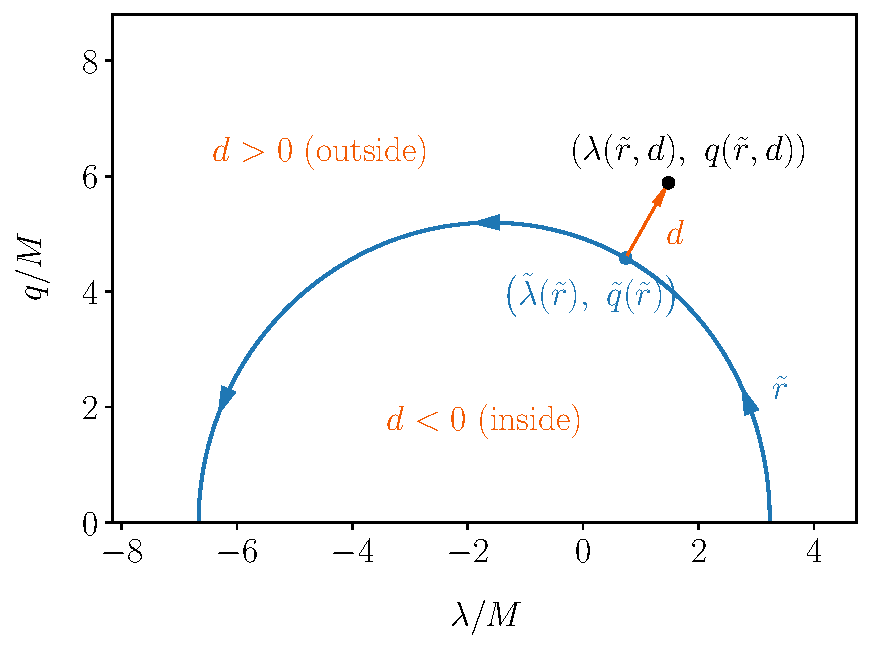
\includegraphics[width=0.48\textwidth]{figures/rc_d_parameterization.pdf}
    \caption{重新参数化求根中使用的测地线守恒定量。所示示例针对的是具有    $a/M = 0.8$    的 BH。蓝色曲线表示对应于边界轨道的临界曲线,箭头表示    $\tilde{r}$    增加的方向。  }
    \label{fig:rc_d parameterization}
\end{figure}     

在实践中,为了高效高精度地识别根,我们将变量    $(\lambda, \eta)$    转换为一对新参数。我们首先引入    $q \equiv \sqrt{\eta}$    ,确保    $\lambda$    和    $q$    具有相同的维数。临界曲线上    $q$    的值表示为    $\tilde{q} \equiv \sqrt{\tilde{\eta}}$    。然后,我们通过参数化
   \begin{equation}
    \begin{pmatrix}
        \lambda  \\ 
        q
    \end{pmatrix} \equiv \begin{pmatrix}
        \tilde{\lambda}  \\  
        \tilde{q}
    \end{pmatrix} + \vec{n}_{\lambda q} d,
\end{equation}    评估    $(\lambda, q)$    与其临界曲线对应物    $(\tilde{\lambda}, \tilde{q})$    的偏差,其中
   \begin{equation}
\begin{aligned}
        \vec{n}_{\lambda q} &\equiv \frac{(\p_{\tilde{r}}\tilde{q}, \  -\p_{\tilde{r}}\tilde{\lambda})^{\mathrm{T}}}{\sqrt{(\p_{\tilde{r}}\tilde{\lambda})^2+(\p_{\tilde{r}}\tilde{q})^2}}  \\  &= \frac{ \left[\tilde{r}^2(3M-\tilde{r}), \   a\tilde{q}(\tilde{r}-M)\right]^{\mathrm{T}}} {\sqrt{\tilde{r}^4(3M-\tilde{r})^2+a^2\tilde{q}^2(\tilde{r}-M)^2}}
\end{aligned}
\end{equation}    表示    $\lambda$    -    $q$    平面上临界曲线    $(\tilde{\lambda}, \tilde{q})$    向外指向的单位法向量。参数    $d$    表示    $(\lambda, q)$    与临界曲线的距离,曲线外部和内部的区域分别由    $d > 0$    和    $d < 0$    区分。这种方法可以将每个点    $(\lambda, q)$    唯一地映射到相应临界曲线的距离    $d$    和半径    $\tilde{r}$   ,如图~    \ref{fig:rc_d parameterization}    所示。鉴于高阶图像渐近接近临界曲线,我们选择    $\log_{10}|d/M|$    作为变量来适应径向运动的渐近行为。然后在    $\tilde{r}$    -    $\log_{10}|d/M|$    平面上进行求根过程,符号变量    $(\nu_r^s, \nu_{\theta}^s, \operatorname{sgn}(d)) = (\pm1, \pm1, \pm1)$    共有八种可能的结合,应逐一求解。对于每种符号变量组合,绘制    $\theta_f = \theta_o$    和    $\phi_f = \phi_o + 2k\pi \  (k\in\mathbb{Z})$    的轮廓,它们的交点表示图像。请注意,对于史瓦西黑洞,由于    $\tilde{r}$    始终为    $3M$    ,因此在    $\log_{10}|d/M|$    的一维空间中找到一个根就足够了。同样,这可以通过限制在赤道平面上、设置    $\eta = 0$    并求解剩余的守恒量    $\lambda$    来实现。有关详细信息,请参阅第    \ref{subsec:Sch distortion}    节。  

   \subsubsection{光的回音  }    
   \label{subsubsec:light echoes}    通常,从    $x^{\mu}_s$    处的光源出发,有无数条满足方程~(    \ref{eq:imaging condition}    ) 的光线,在观察者的图像平面上形成一系列图像。在到达观察者之前,每条光线都会绕黑洞旋转不同的圈数。标记这些光回波的一种方法是引入沿    $\theta$    方向传播的半轨道数,用    $n$    
   \begin{equation}
    n\equiv\frac{G_{\theta}}{G_{\theta}^{\text{half}}},\qquad G_{\theta}^{\text{half}}\equiv\int_{\theta_-}^{\theta_+}\frac{\dd\theta}{\sqrt{\Theta(\theta)}},
    \label{eq:n}
\end{equation}    表示,它与 Ref.~    \cite{Gralla:2019drh}    中的定义相差    $2$    的倍数。非整数    $n$    量化了光子在    $\theta$    方向经历的旅程长度。每当    $n$    增加二,光子就会在    $\theta$    中经历一次完整的振荡。此定义可以连接到半轨道数的整数定义    $N$    ,通过    \begin{equation}
    N=\left\lfloor n \right\rfloor,
    \label{eq:N}
\end{equation}    ,它适当地定义了每个图像的级别。对于直接图像,其定义为其轨迹因重力而弯曲最小的图像,我们有  {    $n < 1$      }  ,其级别是    $N = 0$    。以下高阶图像具有    $N=1,\,2,\,3\ldots$    ,我们将它们称为透镜图像。具有较大    $N$    的高阶图像渐近地接近    $\alpha$    -    $\beta$    平面上的临界曲线。在下文中,我们将主要使用级别数    $N$    来标记每个图像。如果多幅图像具有相同的级别    $N$    ,我们通过按    $n$    递增的顺序排序并按字母顺序为每个图像分配一个附加字母    $(a,\,b,\,c\ldots)$    来区分它们。例如,如果在级别    $N = 7$    处有三幅图像,我们使用    $7a$    、    $7b$    和    $7c$    来表示它们,它们的  { 一半-   }  轨道数    $n$    满足    $n(7a) < n(7b) < n(7c)$    。
   \subsubsection{一个例子  }    
   \label{subsubsec:example}    
   \begin{figure*}[ht!]
    \centering
    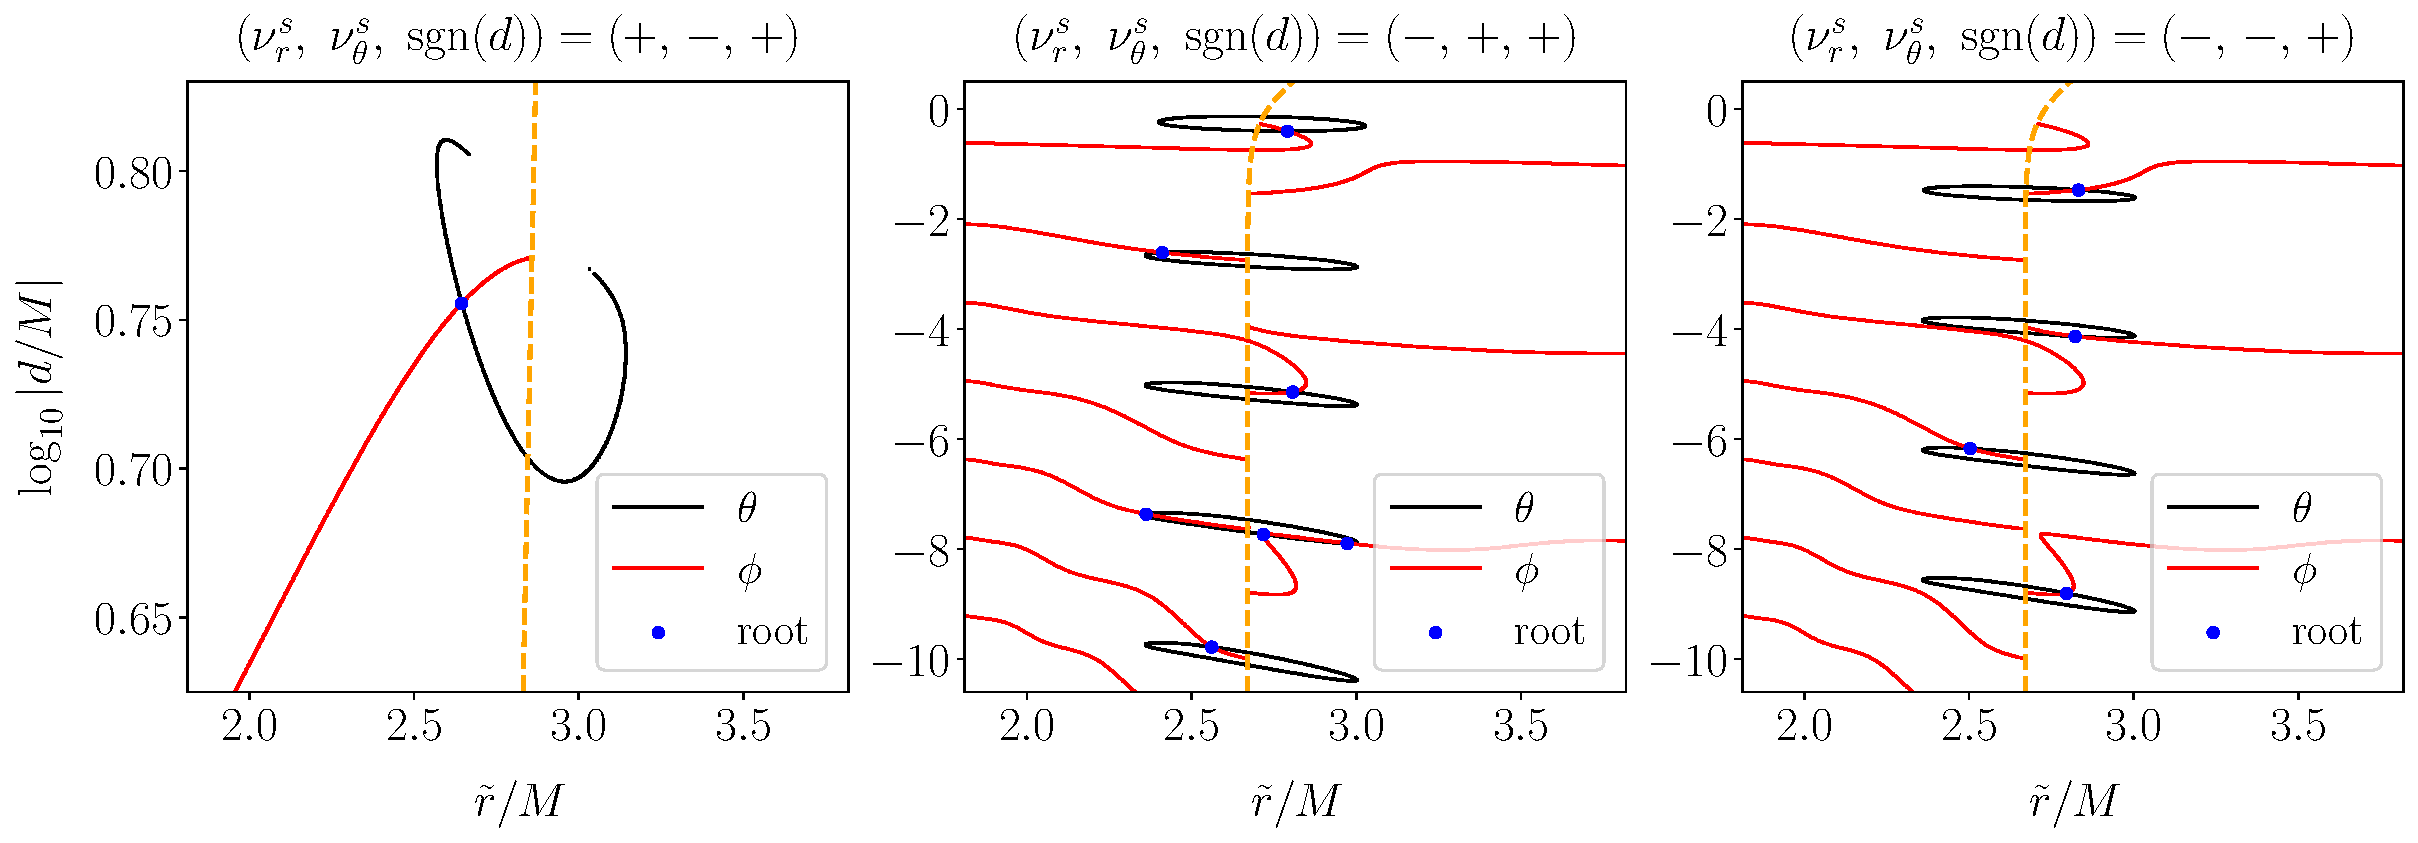
\includegraphics[width=1\textwidth]{figures/contours_combined.pdf}
    \caption{等高线图说明了第 2 节    \ref{subsubsec:example}    中讨论的示例的前向射线追踪中的求根过程:位于自旋为    $a=0.8\,M$    的黑洞外部    $(r_s=10\,M$   、   $\theta_s=\ang{90}$   、   $\phi_s=-\ang{45})$    处的点状源。观察者位于
   $(r_o=1000\,M$   、   $\theta_o=\ang{17}$   、   $\phi_o=0)$    处。   $\lambda = 0$    处的黄色虚线将平面划分为方位角相反的区域:   $\phi_f - \phi_s > 0$   (左)和    $\phi_f - \phi_s < 0$   (右)。黑线和红线分别代表解    $\theta_f = \theta_o$    和    $\phi_f = \phi_o + 2k\pi$   (   $k\in\mathbb{Z}$   ),它们交点处的蓝点对应于光线解。显示了三组解:直接发射(左)和具有对比符号    $\nu_{\theta}^s$    的透镜光子(中和右)。  }
    \label{fig:contour plots}
\end{figure*}     

为了说明我们的前向射线追踪方法的应用,我们考虑一个例子:一个热点位于    $(r_s=10\,M, \theta_s=\ang{90}, \phi_s=-\ang{45})$    处,位于自旋为    $a=0.8\,M$    的 BH 之外,观察者位于    $(r_o=1000\,M, \theta_o=\ang{17}, \phi_o=0)$    处。请注意,   $r_o = 1000\,M$    足够远,对于更大的距离,   $(\lambda, \eta)$    的解几乎保持不变。  

我们首先在图    \ref{fig:contour plots}    中展示了演示根查找过程的轮廓图。黄色虚线标记    $\lambda = 0$   ,将平面分成两个方位角相反的区域:   $\phi_f - \phi_s > 0$   (左)和    $\phi_f - \phi_s < 0$   (右)。黑线和红线分别对应解    $\theta_f = \theta_o$    和    $\phi_f = \phi_o + 2k\pi \  (k\in\mathbb{Z})$   ,蓝点位于它们的交点,对应于前向射线追踪中找到的解。我们的分析确定了满足成像条件方程(   \ref{eq:imaging condition}   )的三组解,按    $(\nu_r^s, \nu_{\theta}^s, \operatorname{sgn}(d))$    的值组织并列在表    \ref{tab:roots}    中。图像位置    $(\alpha, \beta)$    以及假设发射时间    $t_s = 0$    的到达时间    $t_f$    也在表    \ref{tab:roots}    中详细说明。  

在图~   \ref{fig:images}   中,我们展示了相应的测地线和图像。左上面板展示了第~   \ref{subsec:OP}   节中介绍的图像平面,右上面板描绘了各种图像。底部面板显示了与每级图像相对应的轨迹。  

由于源相对于观察者位于黑洞的前景,直接图像来自经历最小引力弯曲的光线,其动量符号为    $\nu_r^s = +1$    和    $\nu_\theta^s = -1$    ,直接反映源和观察者之间的空间配置。另一方面,透镜图像分为两类。对于这两种类型,由于源位于包含束缚轨道的区域之外,因此可以观察到    $\nu_r^s = -1$    ,即    $r_s$    大于    $\tilde{r}_+ \approx 3.82\,M$    ,如方程~(    \ref{eq:bound radius range}    ) 所定义。这两类通过    $\nu_\theta^s$    的对比值来区分。根的    $\log_{10}|d/M|$    值的连续下降表明高阶图像更接近临界曲线。  

透镜图像 (    $N \geq 1$    ) 可以分为两组,这是意料之中的,可以解释如下。透镜图像都是由携带接近临界曲线的守恒量的光线形成的。当它们的轨道在束缚光子轨道附近传播时,它们的轨道接近球形。在史瓦西情况下,接近临界的光子以两个不同的方向进入这些准束缚轨道:顺时针或逆时针。因此,我们预计透镜图像的初始光子方向会自然分成两个簇。我们发现,尽管自旋效应使光子的运动变得复杂,但这种现象在克尔时空中仍然普遍存在。在此处的示例中,两个初始光子簇通过对比    $\nu_\theta^s$    来区分,每个类别中都有奇数和偶数级数    $N$   。请注意,在    $N = 7$    级别,有三个不同的图像,因此我们将它们标记为    $7a$    、    $7b$    和    $7c$    。事实上,在克尔时空中,具有相同    $N$    的多个图像的出现是很常见的,这将在第~    \ref{subsec:image degeneracy}    节中进一步讨论。
   \subsection{光回波的时间延迟和位置角偏移  }    
   \label{subsec:delay and shift}    
   \begin{table*}[htbp]
\centering
\renewcommand\arraystretch{1.3} 
\setlength\tabcolsep{5pt} 
\begin{tabular}{ccc S[table-format=1.5] S[table-format=2.5] c S[table-format=2.2] S[table-format=2.2] S[table-format=4.2] S[table-format=1.3] c}
\hline\hline
\multirow{2}{*}{Type}  & {\hspace{1.8em}}  & \multicolumn{3}{c}{Root} & {\hspace{1.8em}} & \multicolumn{5}{c}{Image}  \\  
                       &    &         $\left(\nu_r^s, \  \nu_{\theta}^s, \  \operatorname{sgn}(d)\right)$         & {        $\tilde{r}/M$        } & {        $\log_{10}\left|d/M\right|$        } &    & {        $\alpha/M$        } & {        $\beta/M$        } & {        $t_f/M$        } & {        $n$        } &         $N$          \\  \hline
direct image:          &    &                 &         &          &    &       &       &         &       &    \\  
                       &    &          $(+, \  -, \  +)$          & 2.64422 &  0.75554 &    & -7.45 & -7.32 & 1007.81 & 0.433 &         $0$          \\ 
lensed images:         &    &                 &         &          &    &       &       &         &       &    \\    
                       &    &          $(-, \  +, \  +)$          & 2.79133 & -0.40197 &    &  1.62 &  5.30 & 1037.38 & 1.590 &         $1$          \\   
                       &    &                 & 2.41127 & -2.61071 &    & -3.76 & -2.58 & 1066.95 & 3.446 &         $3$          \\   
                       &    &                 & 2.80707 & -5.14474 &    &  2.17 & -4.72 & 1097.41 & 5.414 &         $5$          \\   
                       &    &                 & 2.36197 & -7.36752 &    & -4.42 & -0.68 & 1130.81 & 7.485 &         $7a$          \\   
                       &    &                 & 2.97236 & -7.89958 &    &  4.98 &  2.21 & 1131.15 & 7.539 &         $7b$          \\   
                       &    &                 & 2.71788 & -7.73576 &    &  0.74 &  5.00 & 1131.26 & 7.593 &         $7c$          \\   
                       &    &                 & 2.56144 & -9.78463 &    & -1.64 & -4.52 & 1159.67 & 9.411 &         $9$          \\  
                       &    &          $(-, \  -, \  +)$          & 2.83263 & -1.47102 &    &  2.57 & -4.60 & 1050.67 & 2.417 &         $2$          \\   
                       &    &                 & 2.82223 & -4.13481 &    &  2.42 &  4.62 & 1084.52 & 4.584 &         $4$          \\   
                       &    &                 & 2.50343 & -6.17371 &    & -2.47 & -4.01 & 1113.21 & 6.420 &         $6$          \\   
                       &    &                 & 2.79631 & -8.80814 &    &  1.99 & -4.78 & 1144.13 & 8.413 &         $8$          \\   \hline
\end{tabular}
\caption{在    \ref{subsubsec:example}    节中讨论的示例的前向追踪中用    $N \leq 9$    找到的根的列表。根据    $(\nu_r^s,\,\nu_{\theta}^s,\,\operatorname{sgn}(d))$    的不同组合,根分为三类。该表显示它们的图像位置    $(\alpha, \beta)$   、到达时间    $t_f$   (假设发射时间为    $t_s = 0$   )以及在    $\theta$    方向    $n$    上传播的  { 一半-   }  轨道数。每个根都通过其级别号    $N$    来区分。  }
\label{tab:roots}
\end{table*}    我们已经在图~    \ref{fig:contour plots}   、表~    \ref{tab:roots}    和图~    \ref{fig:images}    中演示了前向射线追踪的示例。图~    \ref{fig:images for various spins}    显示了各种 BH 参数和源位置的图像平面的更多示例。从左到右,我们分别选择自旋    $a/M$    作为    $0.1, 0.2, 0.5$    和    $0.8$    。第一行考虑一个靠近 BH 的源,其    $r_s = 1.7\,M$    ,导致所有透镜图像的    $\nu_r^s = +1$    均为    $r_s < \tilde{r}_{-}$    。最后两行考虑位于    $r_s = 10\,M$    的源,第二行用于近乎正面的观察(    $\theta_o = \ang{17}$    ),第三行用于近乎边缘的观察(    $\theta_o = \ang{80}$    )。  

对于观测目的而言,最相关的量是光回波的位置和到达时间,它们编码了有关时空和源位置的信息。测量这些可观测量的一种方法是通过强度波动相关性    \cite{Broderick:2005my,Fukumura:2007xr,Moriyama:2015zfa,Saida:2016kpk,Gralla:2017ufe,Moriyama:2019mhz,Tiede:2020jgo,Hadar:2020fda,Hadar:2023kau}    ,其中可以在不同图像级别检测到发射源的固有时间变化,延迟一定时间。  

比较两个具有连续水平的图像,它们的传播距离不一定相差半个    $\theta$    轨道,如表    \ref{tab:roots}    中的    $n$    值所示。两者之间的    $n$    差异对源位置很敏感。因此,直接图像 (   $N = 0$   ) 和第一个透镜图像 (   $N = 1$   ) 之间的时间延迟和位置角偏移取决于 BH 和源。  

另一方面,级别相差    $2$    的图像通常由一个    $\theta$    轨道分隔,因为它们具有相似的初始方向,由    $\nu_\theta^s$    表征,如表~    \ref{tab:roots}    所示。因此,第    $N$    和第    $(N + 2)$    图像之间的时间延迟主要由 BH
   \begin{equation}
t_f^{N+2} - t_f^N \approx 2\tau,
\end{equation}    的通用属性决定,其中    $\tau \approx 15\,M$    是表征    $\theta$    方向半振动时间周期的关键参数  

   \begin{figure*}[ht]
    \centering
    \begin{minipage}{0.45\textwidth}
        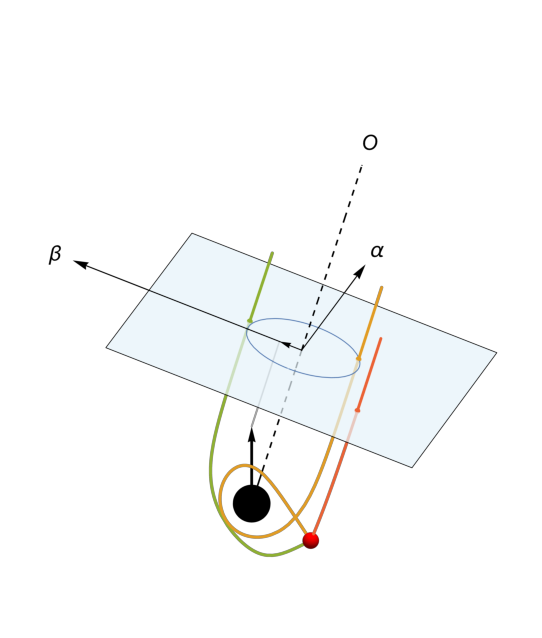
\includegraphics[width=0.95\textwidth]{figures/3D_demo.pdf}
    \end{minipage}
    \quad
    \begin{minipage}{0.45\textwidth}
        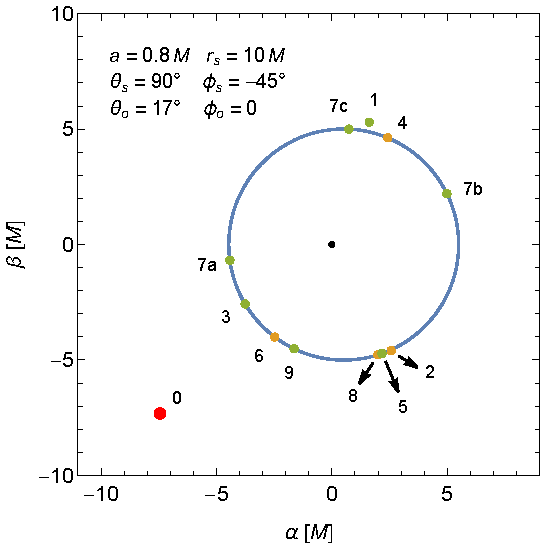
\includegraphics[width=0.95\textwidth]{figures/images.pdf}
    \end{minipage}
    \includegraphics[width=0.8\textwidth]{figures/multiple_images_geodesics_lowR.png}
    \caption{在    \ref{subsubsec:example}    节中讨论的例子中,前向射线追踪中找到的测地线和解的图像。左上角:图像平面    $\alpha-\beta$    的插图,显示了最低三个级别的解。垂直于平面的黑色虚线表示从观察者到黑洞的视线。黑洞上的短黑箭头表示其自旋方向,其投影与平面上的    $\beta$    轴对齐。光线将点源(红色球体)与远处的观察者(   $O$   )连接起来。右上角:以黑洞(黑点)的视线方向为中心的图像平面上点源的图像。直接图像以红色显示,而透镜图像对于    $\nu_{\theta}^s = +1$    为绿色,对于    $\nu_{\theta}^s = -1$    为橙色。临界曲线以蓝色绘制。底部:从    $0$    到    $9$    形成    $N$    图像的光线轨迹。  }
    \label{fig:images}
\end{figure*}     

   \begin{figure*}
    \centering
    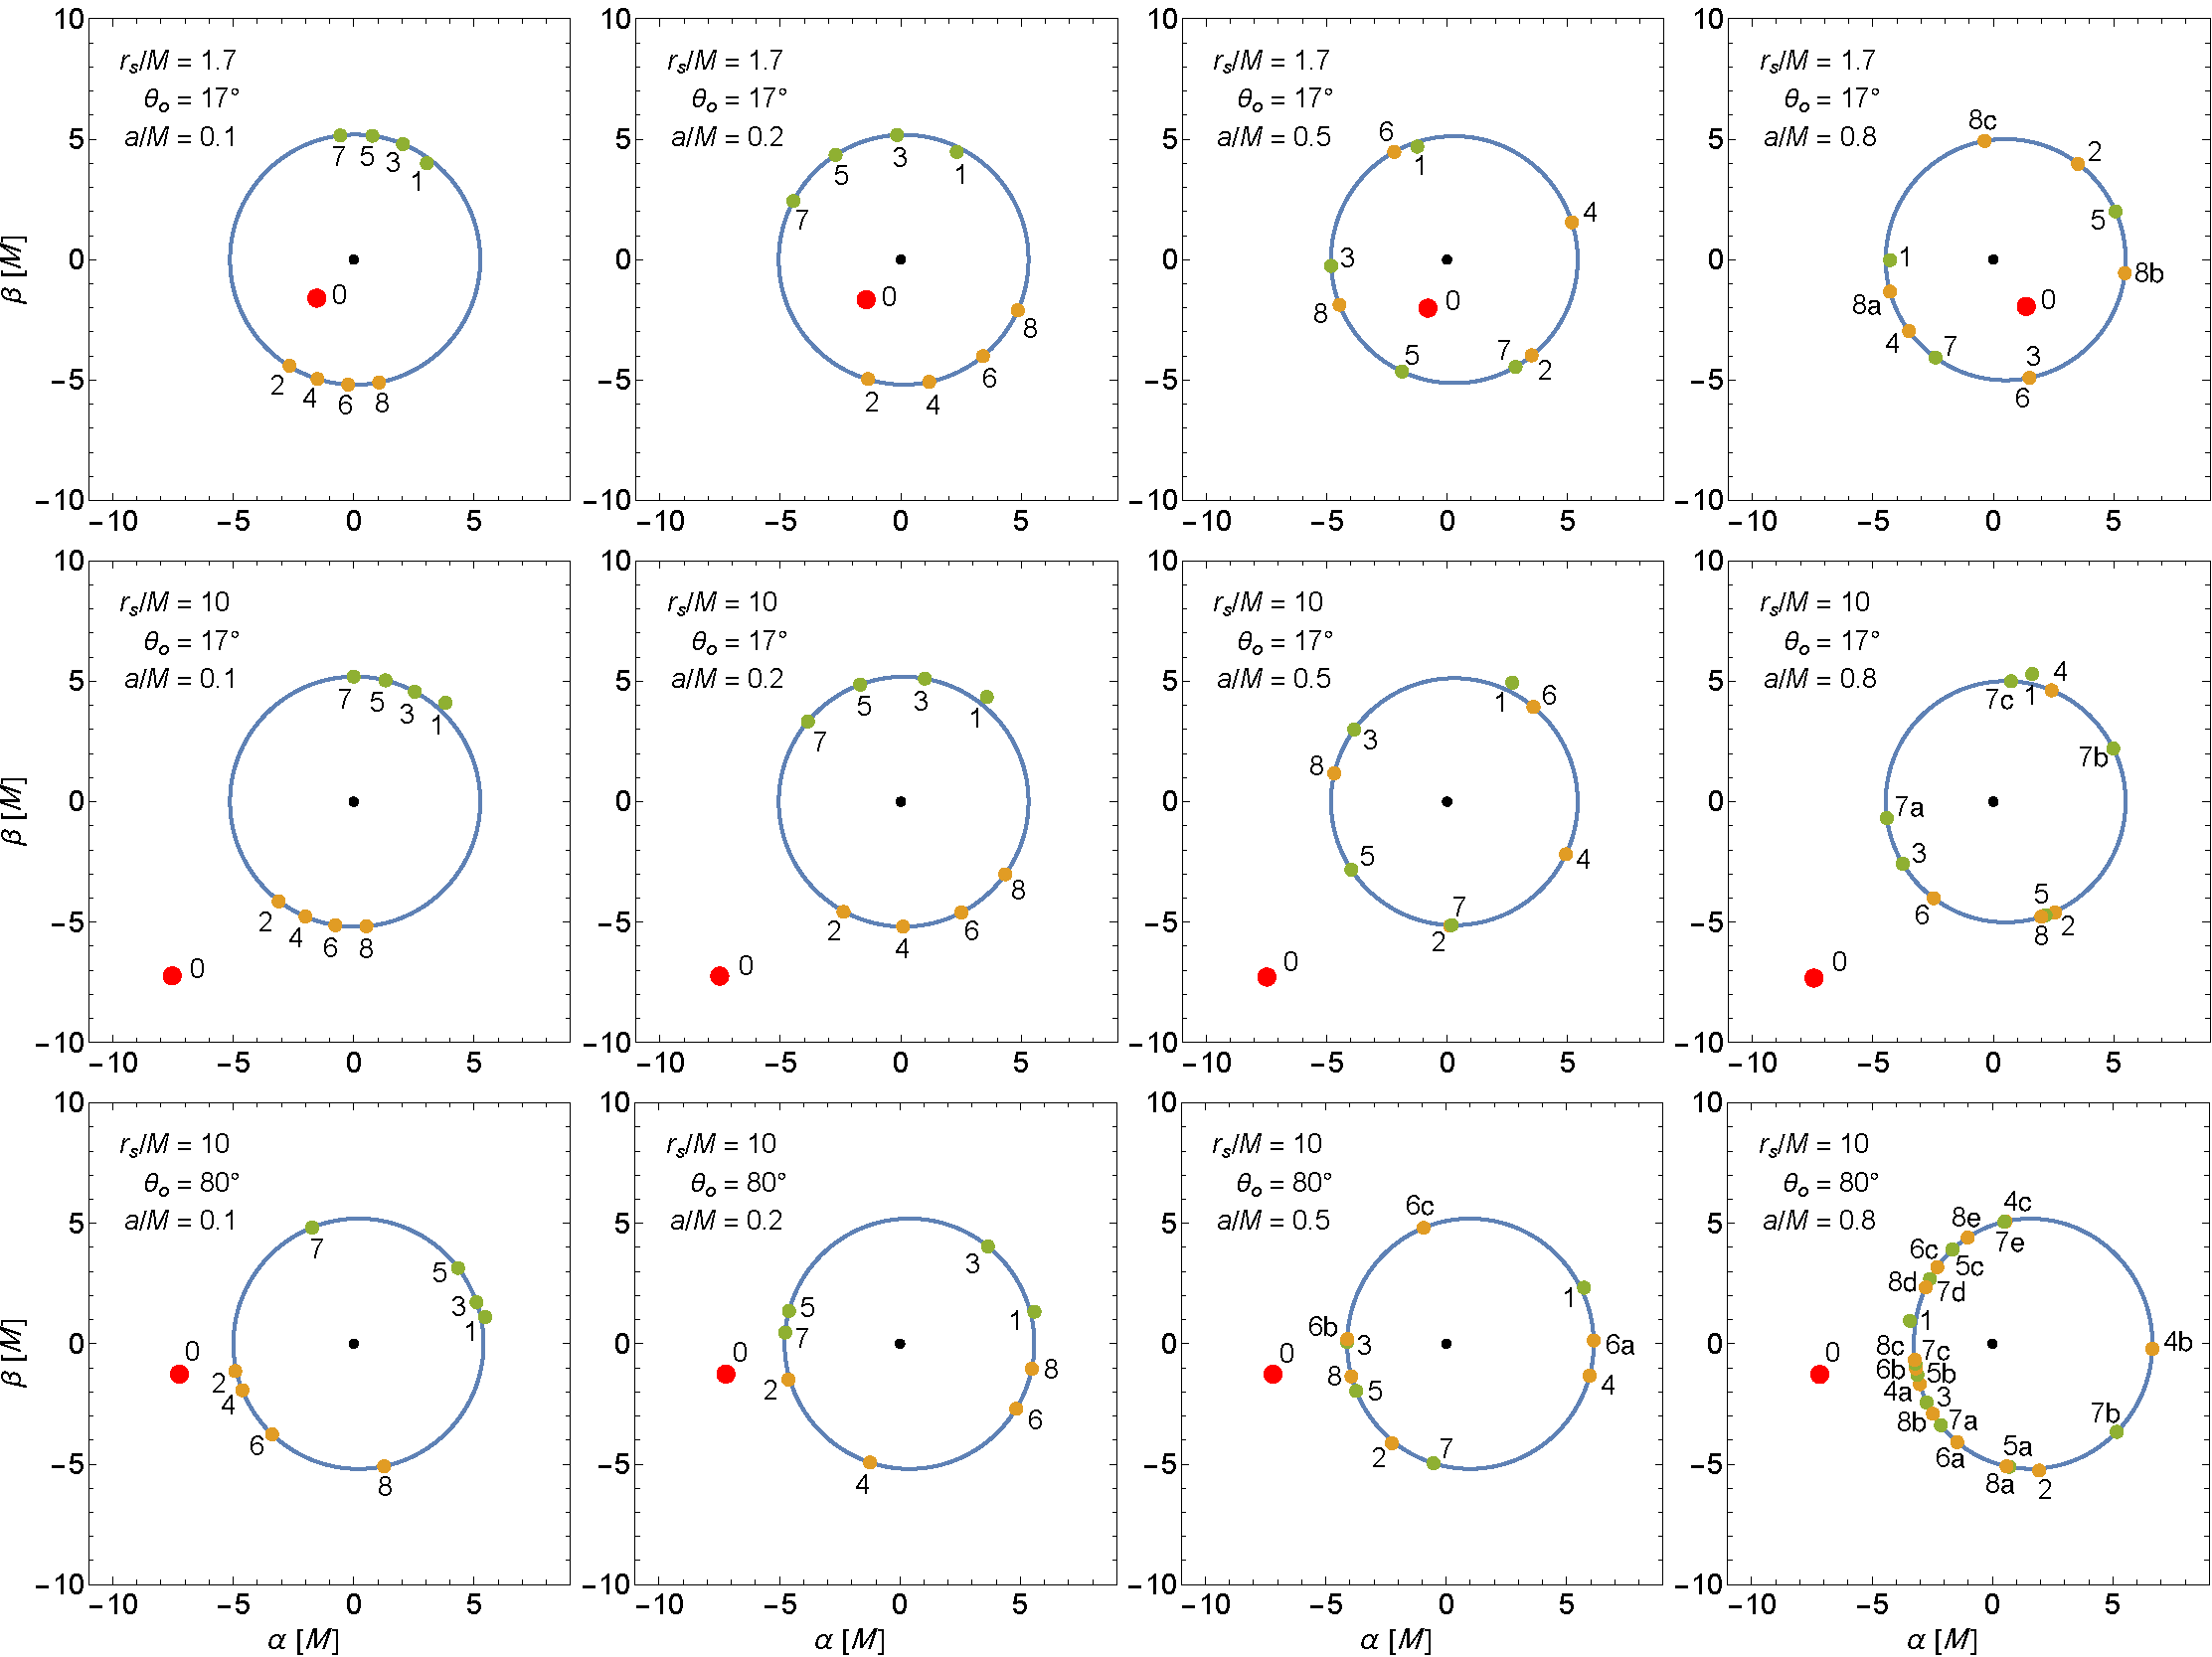
\includegraphics[width=\textwidth]{figures/images_ia_a.pdf}
    \caption{来自不同源位置    $(r_s,\,\theta_s,\,\phi_s)$    、BH 自旋    $a$    和观察者倾斜角    $\theta_o$    的点源的前向射线追踪图像。所有情况下的固定参数为    $\theta_s = \ang{90}$    、    $\phi_s = -\ang{45}$    和    $\phi_o = 0$    。第一行显示    $r_s = 1.7\,M$    处的源,而第二行和第三行分别描述    $r_s = 10\,M$    处的源,倾斜角为    $\theta_o = \ang{17}$    和    $\theta_o = \ang{80}$    。自旋参数    $a/M$    从左到右在各列中从    $0.1, 0.2, 0.5$    到    $0.8$    变化。图像的标签和着色约定遵循图~    \ref{fig:images}    右上面板中使用的约定。为了提高清晰度,特别是在密集排列的面板中,奇数级图像(绿点)的标签位于临界曲线内,而偶数级透镜图像(橙点)的标签则位于临界曲线外。当图像点重叠时,较高级别的图像会叠加在较低级别的图像上。  }
    \label{fig:images for various spins}
\end{figure*}     

   \clearpage     

   \noindent   (从    $\theta_+$    到    $\theta_-$    反之亦然)~    \cite{Gralla:2019drh}    。此参数主要受黑洞质量影响,对于近边缘方向且自旋较高的方向,自旋和倾角有显著修正,尤其是    $\ang{60}\lesssim\theta_o\lesssim\ang{120}$    和    $a\gtrsim 0.9M$    。  

另一个关键参数是半天平动    $\delta$    ~    \cite{Gralla:2019drh}    内的方位角变化。与时间延迟相比,它对黑洞自旋和倾角更敏感。对于正面观察,它的范围从史瓦西黑洞的    $\pi$    到    $a/M = 0.99$    ~    \cite{Gralla:2019drh}    的大约    $3\pi/2$   。有限的倾角,即使小到    $\ang{17}$    ,也会在大自旋下显著变形    $\delta$    ,对于以不同位置角进入束缚轨道的光子会有所不同。从图~    \ref{fig:images for various spins}    中,我们可以看到,随着自旋或倾角的增加,   $N$    和    $2$    相差的图像的位置角偏移变得不那么规则。对于低自旋和近乎正面的观察,位置角偏移的简单关系成立
   \begin{equation}
\varphi^{N+2} - \varphi^N \approx 2\delta - 2\pi,
\end{equation}    为测量黑洞自旋提供了机会。我们将在    \ref{sec:tomography}    节中讨论确定 BH 参数和源位置的更一般情况。
   \subsection{图像级别退化  }   
   \label{subsec:image degeneracy}     

如上一小节所述,点源的同一层    $N$    上可以有多个图像。这种现象不会发生在史瓦西黑洞中,其中每一层的测地线完全位于包含点状源、黑洞和观察者的同一平面内,并沿着一条线依次投影到图像平面上。相反,随着自旋和倾斜角的增加,这种情况变得更加常见。本小节深入探讨这种现象,称为图像级退化。  

除了第 3 节中讨论的例子中的    $7a, 7b$    和    $7c$    能级退化以及图    \ref{fig:contour plots}   、图    \ref{fig:images}    和表    \ref{tab:roots}    中所示的情况外,我们还查看了图    \ref{fig:images for various spins}    的最后一块面板,其中显示了最退化的解。在后一种情况下,源位于具有自旋    $a = 0.8\,M$    的黑洞之外的    $(r_s = 10\,M$   、   $\theta_s = \ang{90}$   、   $\phi_s = -\ang{45})$   ,到达    $(r_o = 1000\,M$   、   $\theta_o = \ang{80}$   、   $\phi_o = 0)$    处的观察者。为了定量地理解这些图像,我们针对上述两种情况,在表    \ref{tab:7abc details}    和    \ref{tab:80deg details}    中分别列出了每幅图像的极方向符号    $\nu_{\theta}^s$   、极半轨道测量值    $n$   、极转动数    $m$    和方位缠绕数    $k \equiv (\phi_f - \phi_o)/(2\pi)$   。  

   \begin{table}[!htbp]
\renewcommand\arraystretch{1.2} 
\setlength\tabcolsep{7pt} 
\centering
\begin{tabular}{ccccc}\hline\hline
Level &         $\nu_{\theta}^s$         &         $n$         &         $m$         &         $k$          \\  \hline
        $7a$         &         $+$         & 7.49 & 7 &         $5$          \\ 
        $7b$         &         $+$         & 7.54 & 8 &         $-3$          \\ 
        $7c$         &         $+$         & 7.59 & 8 &         $-3$          \\  \hline
\end{tabular}
\caption{图~    \ref{fig:contour plots}   、图~    \ref{fig:images}    和表~    \ref{tab:roots}    中退化图像的角运动详细信息,包括极方向符号    $\nu_\theta^s$   、极半轨道测量    $n$   、极转向数    $m$    和方位绕数    $k \equiv (\phi_f - \phi_o)/(2\pi)$   。  }
\label{tab:7abc details}
\end{table}     

   \begin{table}[!htbp]
\renewcommand\arraystretch{1.2} 
\setlength\tabcolsep{7pt} 
\centering
\begin{tabular}{ccccc}\hline\hline

Level &         $\nu_{\theta}^s$         &         $n$         &         $m$         &         $k$          \\  \hline

        $0$         &         $-$         & 0.25 & 0 &         $0$          \\ 

        $1$         &         $+$         & 1.82 & 2 &         $1$          \\ 

        $3$         &         $+$         & 3.08 & 3 &         $2$          \\ 

        $5a$         &         $+$         & 5.06 & 5 &         $-2$          \\ 
        $5b$         &         $+$         & 5.14 & 5 &         $4$          \\ 
        $5c$         &         $+$         & 5.94 & 6 &         $4$          \\ 

        $7a$         &         $+$         & 7.07 & 7 &         $5$          \\ 
        $7b$         &         $+$         & 7.09 & 7 &         $-3$          \\ 
        $7c$         &         $+$         & 7.19 & 7 &         $6$          \\ 
        $7d$         &         $+$         & 7.92 & 8 &         $6$          \\ 
        $7e$         &         $+$         & 7.94 & 8 &         $-3$          \\ 

        $2$         &         $-$         & 2.06 & 2 &         $-1$          \\ 

        $4a$         &         $-$         & 4.11 & 4 &         $3$          \\ 
        $4b$         &         $-$         & 4.44 & 4 &         $-2$          \\ 
        $4c$         &         $-$         & 4.94 & 5 &         $-2$          \\ 

        $6a$         &         $-$         & 6.06 & 6 &         $4$          \\ 
        $6b$         &         $-$         & 6.16 & 6 &         $5$          \\ 
        $6c$         &         $-$         & 6.93 & 7 &         $5$          \\ 

        $8a$         &         $-$         & 8.06 & 8 &         $-3$          \\ 
        $8b$         &         $-$         & 8.07 & 8 &         $6$          \\ 
        $8c$         &         $-$         & 8.22 & 8 &         $7$          \\ 
        $8d$         &         $-$         & 8.92 & 9 &         $7$          \\ 
        $8e$         &         $-$         & 8.94 & 9 &         $6$          \\  \hline
\end{tabular}
\caption{图~    \ref{fig:images for various spins}    的最后一幅图中显示了图像的角运动的详细信息,其符号与表~    \ref{tab:7abc details}    相同。  }
\label{tab:80deg details}
\end{table}     

图~    \ref{fig:contour plots}    和图~    \ref{fig:80deg contours}    显示了每种情况下透镜光子的相应轮廓图。   $\theta_f = \theta_o$    的极坐标轮廓线具有各种闭合环线。鉴于能级数    $N$    是根据在    $\theta$    方向传播的半轨道定义的,如方程~(    \ref{eq:n}    ,    \ref{eq:N}    ) 中所述,每个环对应一个能级。然而,每个环的上部和下部因在    $\theta$    方向的额外转弯而不同。   $\phi_f = \phi_o + 2k\pi$       $(k \in \mathbb{Z})$    的方位角轮廓线以绕组数    $k$    来区分。黄色虚线表示    $\lambda = 0$    轮廓,将透镜光子中的    $k > 0$    和    $k < 0$    区域分隔开。  

根据这些示例中轮廓线的相交方式,我们将图像级别退化的起源分类如下。  

   \begin{itemize}

    \item   额外极地转动。一条方位轮廓线(红色)与一条极地轮廓线(黑色环)在环的上部和下部相交两次。相应的解决方案因方程~(    \ref{eq:m}    ) 中定义的    $\theta$    方向转动数    $m$    而不同。例如,在图~    \ref{fig:images for various spins}    的最后一幅图中,图像    $5b$    和    $5c$    以相同的    $\nu_{\theta}^s$    值开始,但转动数    $m$    不同。它们分别以减小和增加的    $\theta$    传播接近    $\theta_o$   。有关这些图像及其相应轮廓图的更多详细信息,请参阅表~    \ref{tab:80deg details}    和图~    \ref{fig:80deg contours}   (下同)。   \item   相反的方位运动。从左侧和右侧延伸的两个方位轮廓(红色)与一个极轮廓(黑色)相交。此类别中的解决方案因其方位动量的符号不同而不同,以    $k$    的相反符号为特征。例如,图  {    \ref{fig:images for various spins}      }  最后一幅图中的图像    $4a$    和    $4b$    源自两条不同的方位轮廓线。   \item   额外方位角绕组。从同一侧延伸的两个方位角轮廓(红色)与极轮廓(黑色)相交。此类别包括    $k$    符号相同但值不同的情况。一个例子是图    \ref{fig:images for various spins}    最后一页中的图像    $6a$    和    $6b$   。   \item   组合情况。极坐标轮廓(黑色环)与一条或多条方位轮廓(红色)相交,使得额外的极坐标转动与相反的方位运动或额外的方位绕组相重合。   \item   孪生解。方位轮廓(红色)与极轮廓(黑色环)在环的同一部分(上部或下部)相交两次。这些解共享相同的初始    $\theta$    动量符号    $\nu_{\theta}^s$    和转动数    $m$    ,在同一方向上完成相同数量的方位绕圈。因此,它们表现出非常相似的    $n$    值。一个例子是图~    \ref{fig:contour plots}    、图~    \ref{fig:images}    和表~    \ref{tab:roots}    中所示的图像    $7b$    和    $7c$   。  \end{itemize}     

   \begin{figure}[!htbp]
    \centering
    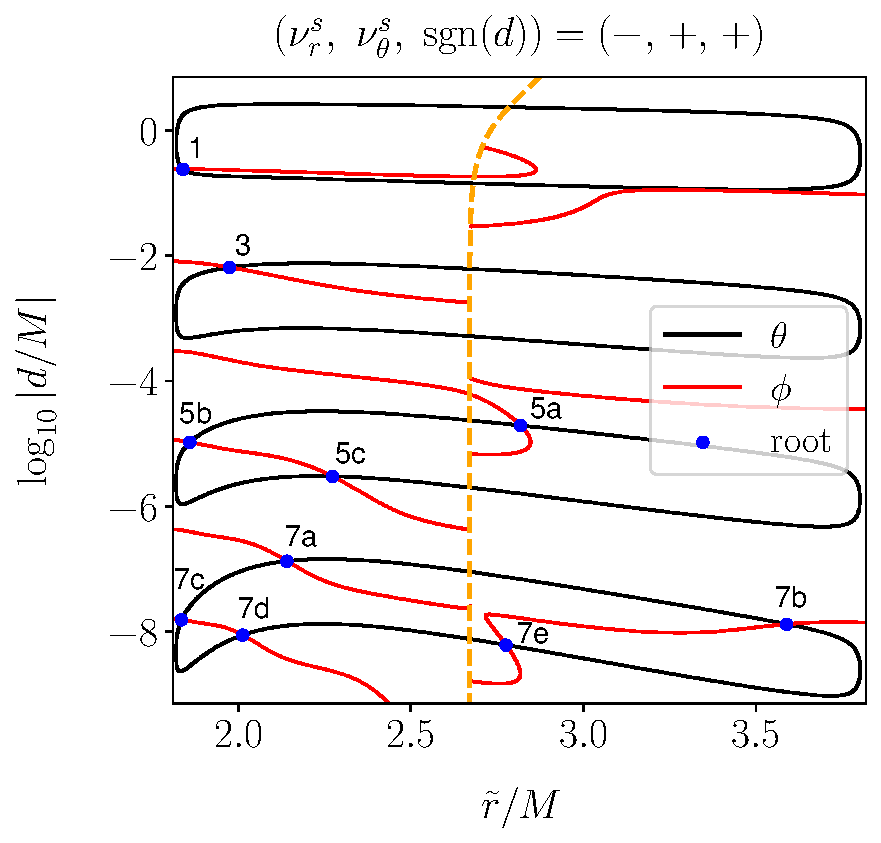
\includegraphics[width=0.4\textwidth]{figures/80deg_contour_1.pdf}
    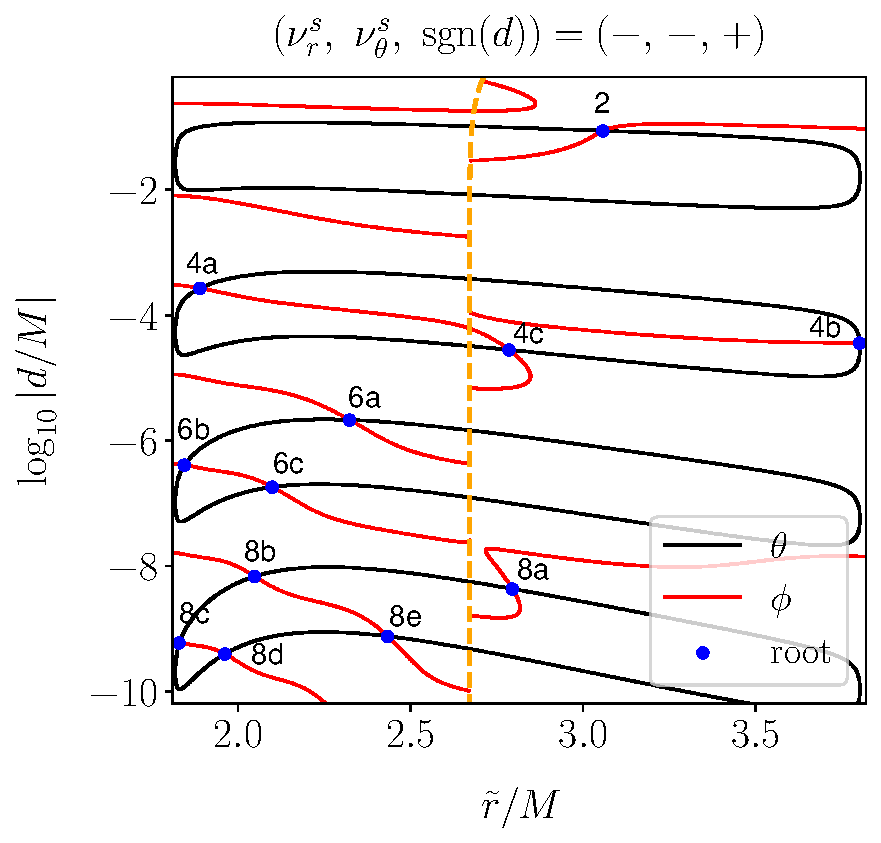
\includegraphics[width=0.4\textwidth]{figures/80deg_contour_2.pdf}
    \caption{用于查找图~    \ref{fig:images for various spins}    最后一个面板中示例的透镜图像的轮廓图,遵循与图~    \ref{fig:contour plots}    相同的符号。  }
    \label{fig:80deg contours}
\end{figure}    
   \section{克尔时空中的图像畸变  }    
   \label{sec:distortion}     

在    \ref{sec:FRLE}    节中开发的前向射线追踪方法可以计算连接 BH 附近特定点和远处观察者的测地线。实际上,发射源(例如热点)具有有限的体积。本节通过介绍一种扰动映射技术来解决这一实际问题。该方法将原始发射点附近的小偏差与图像平面上的相应变化联系起来。我们使用守恒量来制定这种扰动映射,以分析高阶图像沿临界曲线和垂直于临界曲线的放大。然后,我们用史瓦西时空中的一个例子来说明缩放关系,使用简单的几何关系来计算放大因子作为源位置和图像级别的函数。
   \subsection{正向射线追踪的扰动偏差  }     

在我们的前向光线追踪方法中,光线的最终方向    $(\theta_f,\,\phi_f)$    由守恒量    $\lambda$   、   $\eta$   、动量符号    $\nu_r^s$   、   $\nu_{\theta}^s$    和源位置    $\vec{r}_s = (r_s,\, \theta_s,\, \phi_s)$    
   \begin{equation}
\begin{aligned}
\theta_f&=\theta_f\left(\lambda,\,\eta,\,\nu_r^s,\,\nu_{\theta}^s \mid \vec{r}_s\right), \\ 
\phi_f&=\phi_f\left(\lambda,\,\eta,\,\nu_r^s,\,\nu_{\theta}^s \mid \vec{r}_s\right),
\end{aligned}
\end{equation}    决定,其中    $\vec{r}_s$    指定光线的起点,垂直线之前的变量决定其初始方向。  

   \begin{figure}[t]
    \centering
    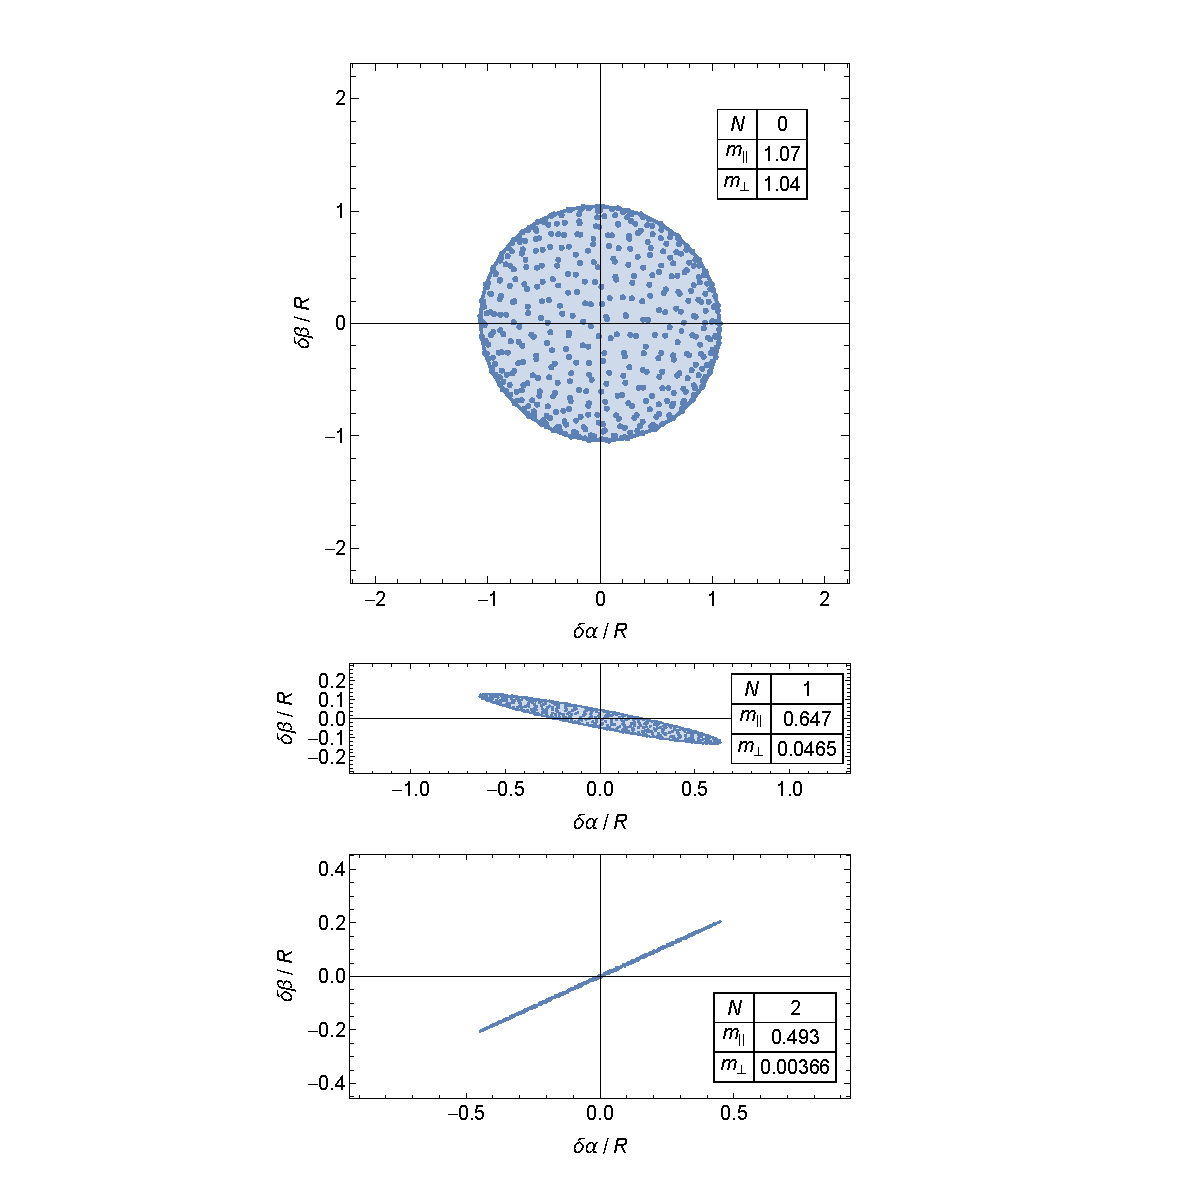
\includegraphics[width=0.45\textwidth]{figures/shapes.pdf}
    \caption{球形发射源的    $N=0, 1$    和    $2$    级图像半径为    $R$    ,中心位于第    \ref{subsubsec:example}    节中描述的发射点,使用相同的 BH 参数。图像平面上的坐标原点对应于发射中心的图像位置。球形源内的采样点是随机选择的,每个采样点在椭圆包络内的图像平面上产生一个蓝点。每个图像级都显示了放大率    $m_{\parallel}$    和    $m_{\perp}$    ,分别定义为这些椭圆的长轴和短轴与    $2R$    的比率。  } 
    \label{fig:shape}
\end{figure}     

   \begin{figure}
    \centering
    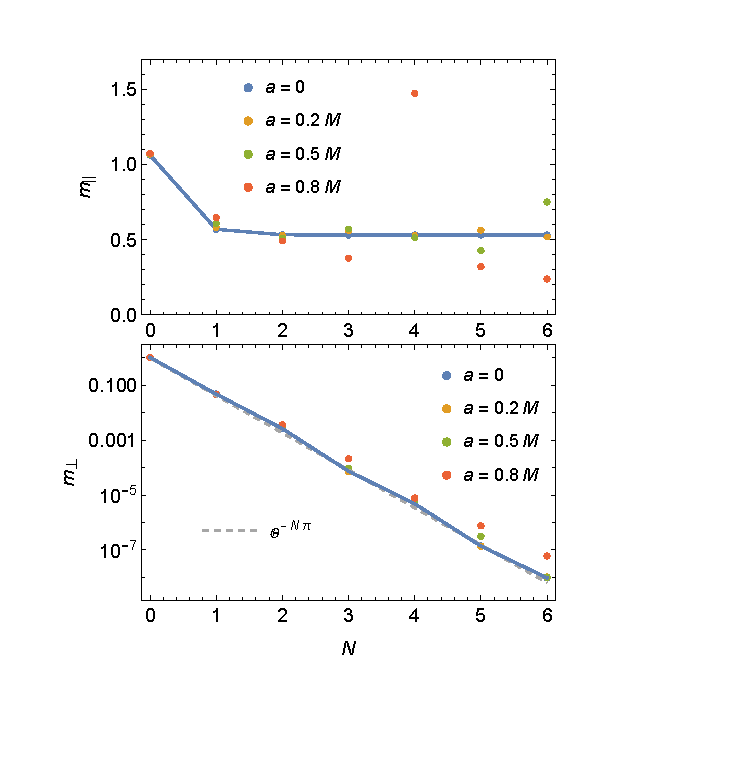
\includegraphics[width=0.45\textwidth]{figures/mags_vs_N.pdf}
    \caption{放大率    $m_{\parallel}$   (顶部)和    $m_{\perp}$   (底部)在不同图像级别    $N$    下绘制,与图    \ref{fig:shape}    中的场景相同,但 BH 自旋不同。这些速率定义为平行于和垂直于临界曲线的椭圆轴与球形源直径 (   $2R$   ) 的比率,显示了图像失真如何随自旋和图像级别而变化。蓝色实线代表史瓦西情况 (   $a=0$   ),而彩色圆点表示不同的自旋值。灰色虚线表示指数缩放    $\propto \ee^{-N\pi}$   。  }
    \label{fig:mag vs. N}
\end{figure}     

在更现实的场景中,发射源占据以    $\vec{r}_s$    为中心的有限体积,源的三维空间扩展映射到每个图像上的二维结构。为了解释这一点,我们在源位置    $\delta \vec{r}_s \equiv (\delta r_s,\,\delta \theta_s,\,\delta \phi_s)$    中引入一个小的位移。为了使来自这个位移点的光线仍然到达    $(\theta_f,\,\phi_f)$    处的观察者,它的初始方向必须相应改变,以守恒量    $\delta \lambda$    和    $\delta \eta$    的偏差为特征。成像条件 (    \ref{eq:imaging condition}    ) 导致
   \begin{equation}
\begin{aligned}
    0&=\delta\theta_{f}=\frac{\p \theta_{f}}{\p \lambda}\delta\lambda+\frac{\p \theta_{f}}{\p \eta}\delta\eta+\frac{\p \theta_{f}}{\p \vec{r}_s}\cdot\delta \vec{r}_s,  \\  
    0&=\delta\phi_{f}=\frac{\p \phi_{f}}{\p \lambda}\delta\lambda+\frac{\p \phi{_{f}}}{\p \eta}\delta\eta+\frac{\p \phi{_{f}}}{\p \vec{r}_s}\cdot\delta \vec{r}_s,
\end{aligned}
\end{equation}    其中    $\p/\p\vec{r}_s \equiv (\p/\p r_s, \p/\p \theta_s, \p/\p \phi_s)$    。由此,我们可以将    $(\delta \lambda,\, \delta \eta)$    解为    $\delta \vec{r}_s$    的线性函数。  

   \begin{figure*}
    \centering
    \includegraphics[width=0.95\textwidth]{figures/mag_distribution.png}
    \caption{放大率    $m_{\parallel}$    和    $m_{\perp}$    分别平行于和垂直于临界曲线,以及面积放大率    $m \equiv m_{\parallel}m_{\perp}$    ,用于史瓦西黑洞外点源的    $N=0$    和    $N=1$    级图像。测地线被限制在    $\theta = \pi/2$    处的    $x$    -    $y$    平面内,观察者位于    $(x=1000\,M, y=0)$    处。为了便于说明,施加了    $y < -0.2\,M$    约束以避免焦散(   $y=0$   )处发散。  }
    \label{fig:mag distribution}
\end{figure*}     

我们进一步使用方程~(    \ref{eq:impact parameters}    ) 将偏差转换为图像位置。结合这些,我们构建了一个扰动映射
   \begin{equation}
    \left(\begin{matrix}
        \delta\alpha  \\  
        \delta\beta
    \end{matrix}\right) = \mathcal{M} \left(\begin{matrix}
        \delta r_s  \\  
        \delta \theta_s  \\  
        \delta \phi_s
    \end{matrix}\right),
\end{equation}   ,其中    $2\times 3$    映射矩阵    $\mathcal{M}$    定义为
   \begin{equation}
    \mathcal{M} \equiv - \begin{pmatrix}
        \dfrac{\p\alpha}{\p\lambda} & \dfrac{\p\alpha}{\p\eta}  \\ [1.1em]
        \dfrac{\p\beta}{\p\lambda} & \dfrac{\p\beta}{\p\eta}
    \end{pmatrix}
    \begin{pmatrix}
        \dfrac{\p\theta_{f}}{\p\lambda} & \dfrac{\p\theta_{f}}{\p\eta}  \\ [1.1em]
        \dfrac{\p\phi_{f}}{\p\lambda} & \dfrac{\p\phi_{f}}{\p\eta}
    \end{pmatrix}^{-1}
    \begin{pmatrix}
        \dfrac{\p\theta_{f}}{\p \vec{r}_s}  \\ [1.1em] 
        \dfrac{\p\phi_{f}}{\p \vec{r}_s} 
    \end{pmatrix}.
    \label{eq:shape matrix}
\end{equation}    这里,   $\p\theta_f/\p\vec{r}_s$    和    $\p\phi_f/\p\vec{r}_s$    都表示行向量,遵循我们对    $\partial/\partial \vec{r}_s$    的定义。利用方程~(    \ref{eq:impact parameters}    ) 中    $\alpha$    和    $\beta$    的定义,以及方程~(    \ref{eq:theta_f}    ) 中    $\theta_f$    的积分公式和方程~(    \ref{eq:integral form}    ,\,    \ref{eq:path integrals}    ) 中    $\phi_f$    的积分公式,可以评估映射矩阵。有关这些计算的实际示例,请参阅    \cite{KerrP2P}    中提供的 Mathematica 笔记本。  

我们考虑一个具有有限球形体积的发射源,其半径为    $R$   ,其关于源中心、黑洞和观察者的时空配置与第节    \ref{subsubsec:example}    中描述的相同。为了确保微扰映射保持有效,球面半径    $R$    必须比    $M$    小得多。通过聚合多个这样的球形体积,可以近似得到更复杂的发射源形状。前三个图像级别(   $N = 0, 1, 2$   )的形状如图~    \ref{fig:shape}    所示。通过将透镜图像(   $N = 1$    和    $N = 2$   )的形状与它们在图像平面上的位置进行比较,如图~    \ref{fig:images}    所示,很明显这些图像通常表现为椭圆形,长轴与临界曲线平行,短轴在垂直方向上显著压缩。放大率    $m_{\parallel}$    和    $m_{\perp}$    分别定义为椭圆轴(平行于和垂直于临界曲线)与源直径    $2R$    的比率。这些比率由映射矩阵    $\mathcal{M}$    的两个奇异值的绝对值决定。图中显示了每个图像级别的放大率。  

我们进一步探索高阶图像和 BH 自旋的影响,在图~    \ref{fig:mag vs. N}    中说明了相应的放大率    $m_{\parallel}$    和    $m_{\perp}$    。蓝线表示带有    $a = 0$    的史瓦西情况。尽管在高自旋时存在偏差,但放大率的总体趋势仍然符合史瓦西情景中观察到的趋势。在下一小节中,我们将使用简单的几何关系推导这些缩放关系,表明    $m_{\parallel}$    在更高水平上大约在    $\mathcal{O}(M/\rho_S)$    处保持相对稳定,其中    $\rho_S = r_s \left|\sin(\phi_o - \phi_s)\right|$    ,而    $m_{\perp}$    随着    $\propto \ee^{-N\gamma} \approx \ee^{-N\pi}$    呈指数下降。  

空间映射在观察热点中起着至关重要的作用,因为每个图像的总强度大致与其面积成正比,这是刘维尔定理~    \cite{Misner:1973prb}    的结果。在图~    \ref{fig:mag distribution}    中,我们展示了对于图像级    $N=0$    和    $N=1$    ,   $m_{\parallel}, m_{\perp}$    和面积放大率    $m \equiv m_{\parallel}m_{\perp}$    如何根据源相对于黑洞和史瓦西时空中观察者的位置而变化。通常,高阶图像会呈指数级变暗,从而带来观察挑战。尽管如此,位于焦散线附近的源可以产生异常放大的图像。  

此外,发射持续时间是一个至关重要的观察参数。对于本文考虑的球形发射模型,我们通过跟踪和比较固定时刻从球体发射的光子的到达时间    $t_f$    的分布来分析时间域中的深度。我们的研究结果证实,每个图像的时间域深度大约等于光子穿过源直径    $2R$    所需的坐标时间。  

   \subsection{史瓦西时空中的图像失真  }    
   \label{subsec:Sch distortion}    本小节使用简单的几何关系推导出史瓦西黑洞外热点的放大率,类似于参考文献~    \cite{Ohanian1987}    中的方法。我们不失一般性地假设,包含热点中心、黑洞和观察者的轨道平面与    $\theta = \pi/2$    处的赤道平面重合。在这些条件下,第~    \ref{subsec:Trajectory}    节中的形式化简化为    $p^{\theta} = 0$    、    $\eta = 0$    、    $\mathcal{R}(r) = r^4 - \lambda^2 r^2(1 - 2M/r)$    和    $\Theta(\theta) = 0$    。为了绕过角积分中的明显奇点,轨道运动被近似为    $\eta \to 0^+$    的极限,这需要    $\theta_{\mp} = \pi/2\,\mp\,\epsilon$    和    $\epsilon \to 0$    之间的无穷小极地振荡。这种近似将方程式    \ref{eq:inteq1}   、   \ref{eq:Gtheta}   、   \ref{eq:Gphi}    中的角度积分简化为    $G_{\theta} = G_{\phi} = \tau$   。该值从方程式    \ref{eq:inteq1}   、   \ref{eq:Ir}    得出,如下所示
   \begin{equation}
    \tau=\fint_{r_s}^{r_f}\frac{\nu_r\dd r}{\sqrt{\R(r)}}=\fint_{r_s}^{r_f}\frac{\nu_r\dd r}{\sqrt{r^4-\lambda^2r^2(1-2M/r)}}.\label{eq:tauS}
\end{equation}    因此,对于史瓦西时空中定义的    $I_{\phi} = 0$   (参见方程式    \ref{eq:Iphi}   ),光子的最终方位角在方程式    \ref{eq:inteq2}    中表示为
   \begin{equation}
\phi_f = \phi_s + \lambda \tau.\label{eq:phifS}
\end{equation}    因此,与方程式    \ref{eq:imaging condition}    相比,成功前向射线追踪的条件简化为    $\phi_f = \phi_o + 2k\pi$   (其中    $k \in \mathbb{Z}$   )。  

   \begin{figure}[!htbp]
    \centering
    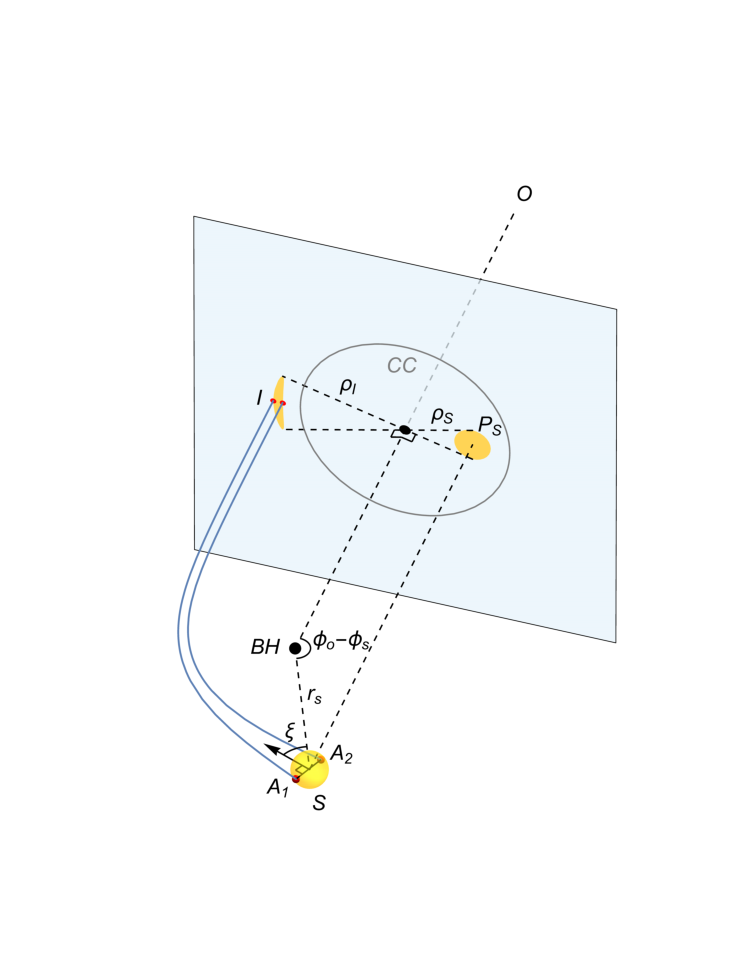
\includegraphics[width=0.45\textwidth]{figures/3D_mag.pdf}
    \caption{球形发射源 (   $S$   ) 及其    $N=1$    级图像 (   $I$   ) 在图像平面上的几何关系说明。   $\rho_I$    和    $\rho_S$    分别表示从图像平面上的 BH 投影到    $I$    和    $S$    的投影 (   $P_S$   ) 的距离。源中心的轨道平面与 BH 赤道平面 (   $\theta=\pi/2$   ) 对齐,位于    $(r_s, \phi_s)$   。从源中心出发的测地线的初始方向由黑色箭头表示,与朝向 BH 的方向形成一个角度    $\xi$   。垂直于临界曲线 (CC) 的两个图像边缘用红点标记,对应于球形源上的点    $A_1$    和    $A_2$   。  }
    \label{fig:3Dmag}
\end{figure}     

为了清楚地说明放大率的推导,我们在图    \ref{fig:3Dmag}    中展示了辐射球形热点的几何关系。热点用    $S$    表示,其中心在    $(r_s,\,\theta_s = 0,\,\phi_s)$    ,从该点开始的测地线的初始方向用黑色箭头表示,指向图像平面上的图像    $I$    。虽然所示示例对    $N=1$    使用测地线,但该解释适用于所有图像级别。黑洞在图像平面上的直接投影作为坐标系的原点,用黑点标记,热点中心的投影标记为    $P_S$    。   $\rho_I = \sqrt{\alpha^2 + \beta^2}$    和    $\rho_S$    分别表示从原点到    $I$    和    $P_S$    的距离。图像平面上标记为“CC”的灰色轮廓线表示临界曲线。  

球形热点内的每个点都形成一个轨道平面,该轨道平面可能与包含源中心的轨道平面不同。我们在图像平面上使用虚线来显示包含轨道平面和图像平面之间相交线的区域的边界。由此,我们可以轻松确定沿临界曲线    \begin{equation}
    m_{\parallel}=\frac{\rho_I}{\rho_{S}}=\left|\frac{\lambda}{r_s\sin(\phi_o-\phi_s)}\right|,
    \label{eq:mpar}
\end{equation}    的放大率,假设热点足够小,即    $R \ll M$    。这里,关系    $\rho_I = \left|\lambda\right|$    来自方程~(    \ref{eq:impact parameters}    ),取    $\theta_o = \pi/2$    和    $\eta = 0$    ,而    $\rho_S = r_s \left|\sin(\phi_o - \phi_s)\right|$    来自简单的几何关系。每个图像级别都以    $\lambda$    为特征,其绝对值在史瓦西情况下随着    $N$    变大而渐近临界值    $|\tilde{\lambda}| = 3\sqrt{3}\,M$    ~    \cite{Luminet:1979nyg}   。  

请注意,当    $\left(\phi_o - \phi_s\right)$    接近    $\pi$    的整数倍时,方程    \ref{eq:mpar}    会发散,这标志着源与黑洞和观察者共线的情况,沿着一条称为焦散线的线。然而,在具有有限大小源的实际场景中,放大率的这种发散受到调节。具体而言,在    $\rho_S = r_s |\sin(\phi_o - \phi_s)| \approx 0$    的对准附近,方程    \ref{eq:mpar}    中    $1/\rho_S$    的明显发散由源投影    $\propto \rho_S \dd \rho_S$    的面积积分补偿,从而对整体强度产生有限的贡献。为了说明起见,考虑一个半径为    $R$    的源,它直接位于焦散线上。总体放大率定义为总图像面积与源投影面积的比率,并以源投影的加权平均值计算,表示为
   \begin{equation}
\begin{aligned}
m_{\text{overall}} &\equiv \frac{\int_0^R m_{\perp} m_{\parallel} \, 2\pi\rho_S \, \dd\rho_S}{\pi R^2}  \\ 
&\simeq \frac{m_{\perp}R \times 2\pi\rho_I}{\pi R^2}  \\  
&= m_{\perp} \frac{2\rho_I}{R}.
\end{aligned}
\end{equation}    因此,总体放大率受比率    $\rho_I/R$    的调节,考虑到源的有限尺寸。  

接下来,我们考虑垂直于临界曲线    $m_{\perp}$    方向的放大率。   $S$    的测地线初始方向与 BH 到源的方向之间的角度定义为    $\xi$    ,遵循几何关系    \begin{equation}
    \tan\xi=\frac{r p^{\phi}}{p^{r}}\bigg\rvert_{S}=\nu_r^s\operatorname{sgn}(\lambda)\frac{1}{\sqrt{r_s^2/\lambda^2-1+2M/r_s}},
    \label{eq:xi}
\end{equation}    ,其中第二个等式可以使用方程式~(    \ref{eq:pr}    ,    \ref{eq:pphi}    ) 得出。这里,   $\lambda$    是来自    $S$    的光线携带的守恒量。  

我们将焦点集中在图像的两个边缘上,在图~    \ref{fig:3Dmag}    的图像平面上用红点标记,这两个边缘源自球面源上的两个点    $A_1$    和    $A_2$    ,其连接线垂直于初始方向。两条测地线以蓝线表示,位于黑洞赤道平面上。    $A_1$    和    $A_2$    的坐标可以参数化为
   \begin{equation}
\begin{aligned}
        \vec{r}_{A_1} &= (r_s+\delta r, \  \pi/2, \  \phi_s+\delta\phi), \\ 
        \vec{r}_{A_2} &= (r_s-\delta r, \  \pi/2, \  \phi_s-\delta\phi),
\end{aligned}
\label{eq:rA1A2}
\end{equation}    其中    $\delta r \equiv R \sin \xi$    和    $\delta \phi \equiv -R \cos \xi / r_s$    。我们分别将它们的守恒量表示为    $\lambda \pm \delta \lambda$    。垂直于临界曲线的图像宽度为    $2|\delta\lambda|$    ,使得放大率为    $m_\perp = |\delta\lambda / R|$    。  

方程~(    \ref{eq:imaging condition}    ) 中条件的方位角部分导致
   \begin{equation}
   0=\delta\phi_{f} = \frac{\p\phi_f}{\p\lambda} \delta\lambda + \frac{\p\phi_f}{\p{r_s}} \delta r_s + \frac{\p\phi_f}{\p{\phi_s}} \delta\phi_s.
    \label{eq:Sch perturbation}
\end{equation}    我们考虑一种特殊情况,其中    $r_s$    和    $\phi_s$    的变化与热点中心的原始测地线对齐,这意味着    $\delta r_s/\delta \phi_s = p^r/p^\phi$    。因此,从这个新位置起源的测地线保留与原始相同的    $\lambda$    ,即    $\delta \lambda = 0$    ,导致关系
   \begin{equation}
    \frac{\p\phi_f}{\p r_s} + \frac{\p\phi_f}{\p \phi_s}\frac{\tan\xi}{r_s} = 0,\label{eq:phifsimp}
\end{equation}    其中使用了方程~(    \ref{eq:xi}    ) 中的关系。接下来,我们考虑与两个边缘点    $A_1$    和    $A_2$    相对应的空间位移。通过将方程~(    \ref{eq:phifsimp}    ) 合并到方程~(    \ref{eq:Sch perturbation}    ) 中并设置    $\delta r_s = \delta r$    和    $\delta \phi_s = \delta \phi$    (如方程~(    \ref{eq:rA1A2}    ) 中所定义),并使用方程~(    \ref{eq:phifS}    ) 所建议的关系    $\partial \phi_f / \partial \phi_s = 1$    ,我们得到
   \begin{equation}
    \delta\lambda=\frac{R}{r_s\cos\xi}\left(\frac{\p\phi_f}{\p\lambda}\right)^{-1}.
\end{equation}    这里,   $\delta \lambda$    表示垂直于临界曲线的图像    $I$    的宽度,从而得到放大率
   \begin{equation}
    m_{\perp}=\left|\frac{1}{r_s\cos\xi}\left(\frac{\p\phi_f}{\p \lambda}\right)^{-1}\right|,
    \label{eq:mperp}
\end{equation}    ,可以使用方程~(    \ref{eq:tauS}    ,    \ref{eq:phifS}    ) 中提供的表达式进一步阐述。  

我们研究了    $m_\perp$    在更高图像级别下的渐近行为。在临界曲线附近,总方位绕组    $\phi_f - \phi_s$    可以近似为~    \cite{Luminet:1979nyg,Gralla:2019xty,Gralla:2019drh,Tsukamoto:2020iez}    
   \begin{equation}
    |\phi_f - \phi_s| \sim \ln\frac{C}{|\lambda-\tilde{\lambda}|},\qquad \lambda\to \tilde{\lambda},
\label{eq:phifphis}
\end{equation}    其中    $C$    是一个数值因子,主要取决于源    $r_s$    的径向位置,它决定了光子经历的路径类型。例如,远离黑洞的源会导致    $C \approx 80.6\,M$    ,而位于地平线外的源会导致    $C \approx 21.6\,M$    ~    \cite{Gralla:2019xty}    。此外,方位绕组随着图像级别    $N$    的增加而近似增加为    $|\phi_f - \phi_s| \sim N\,\pi$    。将其与方程~(    \ref{eq:phifphis}    ) 积分可得出
   \begin{equation}
    \left|\frac{\p\phi_f}{\p\lambda}\right| \sim \frac{1}{|\lambda-\tilde{\lambda}|}\propto \frac{\ee^{N\pi}}{C}.
\end{equation}    将其应用于方程~(    \ref{eq:mperp}    ) 可得出渐近缩放关系
   \begin{equation}
    m_{\perp}\propto\frac{C\,\ee^{-N\,\pi}}{r_s|\cos\xi|},
\end{equation}    ,表明随着    $N$    的增加,高阶图像在垂直于临界曲线的方向上呈指数压缩。该关系还强调,垂直于临界曲线的压缩会因较大的    $r_s$    而加剧。
   \section{时空断层扫描和热点定位  }    
   \label{sec:tomography}    前向射线追踪方法擅长模拟热点图像。本节演示如何应用此方法来获取观测数据,特别是用于从对热点的直接图像 (    $N=0$    ) 和第一个透镜图像 (    $N=1$    ) 的观测中测量黑洞质量、自旋、倾角和热点位置。由于高阶图像的强度受到指数抑制,我们的重点将主要放在这两张初始图像上。  

黑洞附近的发射会表现出明显的时间变化性,这可能会反映在各个图像层面上。这些图像的强度包含了这种变化性,尽管存在特定的时间延迟。因此,通过将图像平面上不同区域的强度波动与相应的时间延迟关联起来,我们可以确认它们的共同来源是来自同一源的发射~    \cite{Hadar:2020fda}    。点状发射的两个最低图像层面之间的时间延迟对黑洞质量敏感,而它们沿光子环的位置角偏移对黑洞自旋敏感~    \cite{Gralla:2019drh,Hadar:2020fda,Andrianov:2022snn}    。此外,观察者对黑洞的倾斜角和热点的空间位置都会影响时间延迟和位置角偏移,使分析复杂化,如第~    \ref{subsec:delay and shift}    节所示。前向光线追踪可以通过促进对各个源位置的扫描来减轻这些复杂性。  

我们模拟一个位于克尔黑洞外部    $(r_s,\theta_s,\phi_s)$    处的点状源,其质量为    $M$   ,自旋为    $a$   ,将连续测地线引向相对于黑洞倾斜角为    $\theta_o$    的观察者。为不失一般性,我们将观察者的方位角设为    $\phi_o = 0$   。通过相关强度的时间变化成功检测热点的直接发射 (    $N=0$    ) 和第一个透镜图像 (    $N=1$    ),我们可以确定这些图像在图像平面上的精确位置,表示为
   \begin{equation}
    (\alpha_0, \beta_0),\quad (\alpha_1, \beta_1),\label{eq:2levels}
\end{equation}    此外,它们到达之间的时间差可以量化为
   \begin{equation}
    \Delta t \equiv t_1 - t_0,\label{eq:2levelst}
\end{equation}    其中    $t_0$    和    $t_1$    分别表示热点同时发射的光子的到达时间,分别对应于    $N=0$    和    $N=1$    图像级别。  

请注意,在方程    \ref{eq:2levels}    中确定图像平面上的位置需要校准图像平面。此校准包括: { (   \romannumeral    1)   }  根据黑洞与观察者之间的距离将角距离转换为长度单位; { (   \romannumeral    2)   }  在黑洞的投影处建立坐标原点; { (   \romannumeral    3)   }  定义自旋投影轴    $\beta$    ,如下面方程    \ref{eq:impact parameters}    所述。对于天体物理黑洞来说,该距离是经过精确测量的,因此不是我们分析的问题。对于几乎正面的观察者,当    $\theta_o$    靠近    $0$    或    $\pi$    时,临界曲线几乎呈圆形,黑洞的投影与其几何中心紧密对齐。因此,与图像位置的不确定性相比,确定坐标原点的不确定性可以忽略不计,因此我们不需要担心。然而,识别自旋投影需要观察黑洞的喷流,而喷流可能并不总是存在。因此,当喷流不可观测时,我们将自旋投影在图像平面上的位置角 (PA) 视为待确定的未知参数。  

   \begin{table}[!htbp]
    \centering
    \renewcommand\arraystretch{1.3} 
    \setlength\tabcolsep{3pt} 
    \begin{tabular}{cc}\hline\hline
         BH and Observer & Source  \\  \hline
        mass         $M$          & \multirow{4}{*}{\makecell[c]{location  \\          $(r_s,\theta_s,\phi_s)$        }}  \\  
        spin         $a$         &  \\  
        inclination angle         $\theta_o$         &  \\  
        PA of spin projection &  \\  \hline
    \end{tabular}
    \caption{通过观察热点的    $N=0$    和    $N=1$    图像来确定参数,包括 BH 和观察者相关量以及源位置。`PA' 是指位置角。  }
    \label{tab:tomoparameters}
\end{table}     

我们在表    \ref{tab:tomoparameters}    中总结了所有需要确定的相关参数,包括与 BH 和观察者相关的量以及源的位置。我们将探讨如何利用(   \ref{eq:2levels}   、   \ref{eq:2levelst}   )中列出的观测数据来确定这些参数。我们的讨论将分为两种情况,取决于我们对 EHT 和 ngEHT 观测到的目标 SMBH 的先验知识程度。  

表    \ref{tab:tomoparameters}    中列出的变量可以使用蒙特卡洛马尔可夫链 (MCMC) 模拟进行估算。我们将随机变量集定义为
   \begin{equation}
\bm{\Theta} \equiv \left(M, \  a, \  \theta_o, \  \text{PA}, \  r_s^{(j)}, \  \theta_s^{(j)}, \  \phi_s^{(j)}, \  \cdots \right)
\label{eq:Theta}
\end{equation}   ,将热点的可观测量定义为
   \begin{equation}
\bm{X}^{(j)} \equiv \left(\alpha_0^{(j)}, \  \beta_0^{(j)}, \  \alpha_1^{(j)}, \  \beta_1^{(j)}, \  \Delta t^{(j)} \right),
\label{eq:Xj}
\end{equation}   ,其中    $j=a,b,c,\ldots$    标记观察到的第    $j$    个热点。每次选择    $\bm{\Theta}$    都会通过前向射线追踪方法生成直接图像和第一个透镜图像    $\bm{X}^{(j)}(\bm{\Theta})$   。然后将它们与观测值    $\overbar{\bm{X}^{(j)}}$    进行比较,在以下两个示例中,假设观测值与根据真实参数计算出的理论值相匹配。因此,我们引入似然函数
   \begin{equation}
    p\left(\bm{X}\middle|\bm{\Theta}\right) = \prod_{k,j}\frac{1}{\sqrt{2\pi}\sigma_{\bm{X}_k^{(j)}}}\exp\left[-\frac{(\bm{X}^{(j)}_k(\bm{\Theta})-\overbar{\bm{X}^{(j)}_k})^2}{2\sigma_{\bm{X}_k^{(j)}}^{2}}\right],
\end{equation}   ,其中    $k$    标记向量    $\bm{X}^{(j)}$    的每个分量,   $\sigma_{\bm{X}_k^{(j)}}$    对应于其测量不确定度。  

在    $\bm{\Theta}$    中的某些变量由其他测量预先确定的情况下,例如倾角    $\theta_o$    、自旋投影 PA 和 SMBH 质量    $M$    ,我们采用先验概率函数
   \begin{equation}
    p(\bm{\Theta}) = \prod_{l} \frac{1}{\sqrt{2\pi}\sigma_{\bm{\Theta}_l}}\exp\left[-\frac{(\bm{\Theta}_l-\overbar{\bm{\Theta}_l})^2}{2\sigma_{\bm{\Theta}_l}^2}\right],
\end{equation}    ,其中    $l$    将预先确定的参数标记为真实值    $\overbar{\bm{\Theta}_l}$    和不确定性    $\sigma_{\bm{\Theta}_l}$    。根据贝叶斯定理,后验概率为
   $p\left(\bm{\Theta}\middle|\bm{X}\right)\propto p\left(\bm{X}\middle|\bm{\Theta}\right) p(\bm{\Theta})$    。  

Python 包 emcee ~    \cite{Foreman_Mackey_2013}    用于 MCMC 模拟。在模拟过程中,我们允许    $\bm{\Theta}$    从其真实值开始变化。然后使用所得图像和时间延迟的分布来计算后验概率。我们将观察者距离固定在    $r_o=1000\,M$    处,结果已收敛到较大距离处的结果。  

在接下来的两个小节中,我们将分析两个目标超大质量黑洞 M87    $^*$    ~    \cite{EventHorizonTelescope:2019ggy}    和 Sgr A    $^*$    ~    \cite{EventHorizonTelescope:2022exc}   ,利用 EHT 的现有能力可以探测到周围的热点,预计其下一代升级将更有前景。  

   \subsection{M87    $^*$    具有预定的 PA 和    $\theta_o$     }    
   \label{subsec:M87}     

对 M87    $^*$    喷流的观测已确定自旋投影和    $\theta_o = {(163\pm 2)}^\circ$    ~    \cite{EventHorizonTelescope:2019pgp}    的 PA。因此,在表~    \ref{tab:tomoparameters}    中仍有    $5$    个参数需要确定,包括黑洞质量和自旋,以及热点位置(假设只有一个热点观测)。这个未知数的数量与方程~(    \ref{eq:Xj}    ) 中为单个热点的两个最低级图像提供的可观测量数量相匹配,从而允许对热点进行成功的相关观测,从而可能确定所有相关参数。  

考虑一个黑洞的例子,它的质量为    $\overbar{M}$    ,自旋为    $\overbar{a/M} = 0.8$    ,热点在    $(\overbar{r_s},\,\overbar{\theta_s},\,\overbar{\phi_s}) = (10\,\overbar{M},\,\ang{90}, \  \ang{-45})$    ,从    $\phi_o = 0$    和    $\overbar{\theta_o} = \ang{163}$    与    $\sigma_{\theta_o} = \ang{2}$    观察到。使用前向射线追踪,发射    $N=0$    和    $N=1$    的撞击参数的对应真实值分别为    $(\overbar{\alpha_0},\,\overbar{\beta_0}) = (-7.45\,\overbar{M},\, 7.32\,\overbar{M})$    和    $(\overbar{\alpha_1},\,\overbar{\beta_1}) = (1.62\,\overbar{M},\, -5.30\,\overbar{M})$    ,时间延迟为    $\overbar{\Delta t} = 29.57\,\overbar{M}$    。如前所述,可观测量的中心值设置为与它们的理论真实值相匹配。我们假设    $N=0$    和    $N=1$    的测量不确定性为    $\sigma_{\alpha_0} = \sigma_{\beta_0} = \overbar{M}$    和    $\sigma_{\alpha_1} = \sigma_{\beta_1} = 2\,\overbar{M}$    ,反映了 ngEHT~    \cite{Chael:2021rjo,Lico:2023mus}    预期的角分辨率,时间分辨率为    $\sigma_{\Delta t} = 0.5\,\overbar{M}$    。这些参数和不确定性列于表    \ref{tab:set M87}    中。  

   \begin{table}[!htbp]
\renewcommand\arraystretch{1.3} 
\setlength\tabcolsep{2.5pt} 
\begin{tabular}{cc|cccc}
\hline\hline
Parameter & Truth & & Observable & Measurement & Uncertainty  \\  \hline
         $M$         &         $\overbar{M}$          & &         $\alpha_0$         &         $-7.45\,\overbar{M}$         &         $\overbar{M}$          \\  
         $a/M$         &         $0.8$         & &         $\beta_0$         &         $7.32\,\overbar{M}$         &         $\overbar{M}$          \\  
         $r_s/M$         &         $10$          & &         $\alpha_1$         &         $1.62\,\overbar{M}$         &         $2\,\overbar{M}$         \\  
         $\theta_s$         &         $\ang{90}$          & &         $\beta_1$         &         $-5.30\,\overbar{M}$         &         $2\,\overbar{M}$         \\ 
         $\phi_s$         &         $\ang{-45}$          & &         $\Delta t$         &         $29.57\,\overbar{M}$         &         $0.5\,\overbar{M}$         \\  \hline
\end{tabular}
\caption{左图:M87 外部热点    $^*$    的待确定参数及其假定真值;右图:热点发射的    $N=0$    和    $N=1$    光子的可观测量,以及它们的测量值(假定与理论真值相符)和测量不确定性。自旋投影 PA 和    $\theta_o = {(163\pm 2)}^\circ$    是预先确定的。  }
\label{tab:set M87}
\end{table}     

图~   \ref{fig:mc_M87}    展示了 MCMC 模拟的结果,使用 Python 包 GetDist ~   \cite{Lewis:2019xzd}    进行可视化。正如预期的那样,参数的真实值落在    $1\sigma$    可信区间内。该方法通过一次观察分别估计黑洞质量和自旋,精度在    $5 \% $    和    $40 \% $    之内,而无需假设源位置或倾角。多次独立观察可以按其数量的平方根成比例地提高此分辨率。  

   \begin{figure*}
    \centering
    \includegraphics[width=0.9\textwidth]{figures/mc_M87_dpi800_compressed.png}
    \caption{通过观察 M87    $^*$    外部热点的    $N=0$    和    $N=1$    光子得出 BH 和热点位置参数的后验分布,如表~    \ref{tab:set M87}    所示。自旋投影 PA 和    $\theta_o = {(163\pm 2)}^\circ$    被纳入为预先确定的先验。红线表示真实值。在对角线上,中间的虚线标记了分布的模式,两侧的虚线划定了    $1\sigma$   (   $68.3 \% $   )可信区间。确定的值及其不确定性列在每个图的顶部。非对角线上的等高线代表    $1\sigma$   (   $39.3 \% $   )和    $2\sigma$   (   $86.4 \% $   )可信区域。  }
    \label{fig:mc_M87}
\end{figure*}    
   \subsection{Sgr A    $^*$    具有未确定的 PA 和    $\theta_o$     }    
   \label{subsec:SgrA}     

由于缺乏对 Sgr A    $^*$    的喷流观测,因此很难确定其自旋投影 PA 和倾角。尽管 GRAVITY 合作组织最近的观测表明    $\theta_o \sim \ang{157}$    ~    \cite{GRAVITY:2023avo}    更受青睐,但在本小节中,我们将其视为未确定的,以证明独立的 EHT/ngEHT 测量能够通过热点相关推断这些参数。与第 2 节中描述的情形不同,提供    $5$    约束的单个热点观测不足以解决 Sgr A    $^*$    的所有    $7$    未知参数。至少需要两次独立观测,从而产生    $10$    约束,这与未知数的数量相匹配。考虑到 Sgr A    $^*$    周围热点出现的频率(可能每天一次),这一要求在实践中是可行的。  

为了适应未确定的自旋投影 PA,我们在图像平面上引入了一个笛卡尔坐标系    $(X,\,Y)$   ,它通过旋转变换与    $(\alpha,\,\beta)$    坐标相关
   \begin{equation}
    \begin{pmatrix}
        X  \\  Y
    \end{pmatrix} = \begin{pmatrix}
    \cos\PA & -\sin\PA  \\  
    \sin\PA & \cos\PA
    \end{pmatrix} \begin{pmatrix}
        \alpha  \\  \beta
    \end{pmatrix}.
    \label{eq:XY}
\end{equation}    对于每个热点,   $N=0$    和    $N=1$    图像的位置分别用    $(X_0^{(j)},\,Y_0^{(j)})$    和    $(X_1^{(j)},\,Y_1^{(j)})$    表示,相应的时间延迟为    $\Delta t^{(j)}$   。  

数学家协会  

表~   \ref{tab:SgrA}    显示了两个涉及 Sgr A    $^*$    的例子的 BH 时空参数和热点位置的假定真值。右侧列出了可观测量的相应真值和测量不确定性。图~   \ref{fig:mcSgrA}    所示的 MCMC 结果证明,大多数参数(如 BH 质量和自旋)都得到了有效约束,显示出具有明显中心峰值的后验分布;真值落在    $1\sigma$    可信区间内。然而,准确确定    $\theta_o$    更加困难,因为它的真实值位于    $1\sigma$    区间之外。之所以出现这一挑战,是因为当    $\theta_o$    几乎正面对着    \cite{Gralla:2019drh,Hadar:2020fda}    时,   $N=0$    和    $N=1$    光子之间的位置角偏移和时间延迟都仅受到    $\theta_o$    的轻微影响。这种简并性可以通过多次热点相关观测来缓解。类似地,随着独立热点观测数量的增加,测量黑洞质量和自旋等宇宙时空参数的精度预计会提高,这对 Sgr A    $^*$    来说是一个希望。  

   \begin{figure*}
    \centering
    \includegraphics[width=0.95\textwidth]{figures/mc_SgrA_ex2_v2_compressed.png}
    \caption{从人马座 A    $^*$    外两个热点的    $N=0$    和    $N=1$    光子的观测中获得的 BH 和热点位置参数的后验分布,包括自旋投影 PA 和    $\theta_o$   ,如表~    \ref{tab:SgrA}    中所述。此图的符号与图~    \ref{fig:mc_M87}    中使用的符号一致。  }
    \label{fig:mcSgrA}
\end{figure*}    
   \section{讨论  }       \label{sec:dis}     

连接克尔时空中两个空间点的零测地线可以呈现多个解,这归因于黑洞的强引力透镜效应。本研究开发了一个系统框架来识别这些解,并根据围绕黑洞运行的轨道数对它们进行分类。每条测地线都由其在克尔时空中的守恒量和初始动量符号唯一确定。  

该方法的直接应用是 BH 成像,特别是将 BH 外部的点状发射源连接到远处的观察者。这种新颖的前向射线追踪方法被证明比传统的后向射线追踪更有效,特别是在建模热点和计算高阶图像方面。通过对发射点周围的原始测地线应用扰动调整,我们的方法可以将有限尺寸的发射映射到观察者平面上的不同区域。高阶图像通常位于临界曲线附近,在垂直于曲线的方向上依次压缩,同时保持与曲线平行的稳定放大率。因此,随着图像级别    $N$    的增加,总面积放大率呈现指数衰减。  

我们的方法对时空断层扫描很有帮助,特别是对于测量黑洞自旋和质量。利用 EHT 和 ngEHT 捕获的直接图像和透镜图像,我们的方法可以精确确定黑洞特性。对于 M87    $^*$    ,由于自旋投影和倾角是预定的,所以一次测量就足以分辨出黑洞的质量、自旋和发射位置。对于 Sgr A    $^*$    ,两次独立的热点相关性测量足以确定所有相关参数。鉴于 Sgr A    $^*$    周围热点每天都会发生耀斑,成功探测的前景一片光明,尤其是使用 ngEHT,它将提供热点运动跟踪~    \cite{Emami:2022ydq}    和多频率测量能力~    \cite{Chael:2022meh}    。随着更多数据的积累,确定通用时空参数的准确性将会提高。  

重要的是,前向射线追踪方法不仅限于光子,还扩展到引力波,引力波也遵循几何光学极限中的零测地线。例如,超大质量黑洞附近的恒星质量黑洞双星发射的引力波可以通过直接和透镜测地线产生回声~    \cite{Chen:2017xbi,DOrazio:2019fbq,Gondan:2021fpr,Basak:2022fig,Savastano:2022jjv,Zhang:2024ibf,Kubota:2024zkv}    。超大质量黑洞双星在旋涡阶段也可能表现出自透镜特征~    \cite{DOrazio:2017ssb, Ingram:2021gar, Kelley:2021yfc}    。我们的方法可以预测这些事件中引力波信号的调制,从而揭示它们的轨道动力学。  

鉴于我们的方法利用了克尔时空中的守恒量,一个有趣的问题出现了:前向射线追踪是否可以适用于受扰动的时空,例如具有度量扰动的时空~    \cite{Giddings:2016btb, Giddings:2019jwy, Wang:2019skw, Chen:2022kzv, Zhu:2023omf,Zhong:2024ysg}    ?此外,探索前向射线追踪和辐射传输之间的相互作用可以产生深刻的见解,特别是对于极化信号的传播~    \cite{Chen:2019fsq, Himwich:2020msm, Chen:2021lvo, Chen:2022oad}    。  

   \hspace{5mm}    
   \begin{acknowledgments}我们感谢 Xian Chen、Daniel D'Orazio、Shahar Hadar、Yosuke Mizuno、Daniel Palumbo、Diogo Ribeiro、Paul Tiede、Luka Vujeva、Bo Wang、George Wong 和 Xiao Xue 的有益讨论。L.Z. \  感谢北京大学为其访问尼尔斯·玻尔研究所提供的资金支持。Z.Z. \  感谢中国国家留学基金委 (No.~202106040037) 的资金支持。V.C. \  是 Villum 研究员和 DNRF 主席。我们感谢 VILLUM 基金会 (拨款编号 VIL37766) 和丹麦国家研究基金会的 DNRF 主席计划 (拨款编号 DNRF162) 的支持。我们感谢欧盟 H2020 ERC 高级拨款“黑洞:发现的引力引擎”拨款协议编号提供的资金支持。 Gravitas–101052587。但所表达的观点和意见仅代表作者本人,并不一定反映欧盟或欧洲研究理事会的观点和意见。欧盟和授权机构均不对此负责。该项目已获得欧盟“地平线 2020”研究和创新计划的资助,资助协议编号为 101007855 和 101131233。  \end{acknowledgments}     

   \begin{thebibliography}{139}
\makeatletter
\providecommand \@ifxundefined [1]{
 \@ifx{#1\undefined}
}
\providecommand \@ifnum [1]{
 \ifnum #1\expandafter \@firstoftwo
 \else \expandafter \@secondoftwo
 \fi
}
\providecommand \@ifx [1]{
 \ifx #1\expandafter \@firstoftwo
 \else \expandafter \@secondoftwo
 \fi
}
\providecommand \natexlab [1]{#1}
\providecommand \enquote  [1]{``#1''}
\providecommand \bibnamefont  [1]{#1}
\providecommand \bibfnamefont [1]{#1}
\providecommand \citenamefont [1]{#1}
\providecommand \href@noop [0]{\@secondoftwo}
\providecommand \href [0]{\begingroup \@sanitize@url \@href}
\providecommand \@href[1]{\@@startlink{#1}\@@href}
\providecommand \@@href[1]{\endgroup#1\@@endlink}
\providecommand \@sanitize@url [0]{\catcode ` \\ 12\catcode ` \$ 12\catcode ` \& 12\catcode ` \# 12\catcode `\^12\catcode `\_12\catcode ` \% 12\relax}
\providecommand \@@startlink[1]{}
\providecommand \@@endlink[0]{}
\providecommand \url  [0]{\begingroup\@sanitize@url \@url }
\providecommand \@url [1]{\endgroup\@href {#1}{\urlprefix }}
\providecommand \urlprefix  [0]{URL }
\providecommand \Eprint [0]{\href }
\providecommand \doibase [0]{http://dx.doi.org/}
\providecommand \selectlanguage [0]{\@gobble}
\providecommand \bibinfo  [0]{\@secondoftwo}
\providecommand \bibfield  [0]{\@secondoftwo}
\providecommand \translation [1]{[#1]}
\providecommand \BibitemOpen [0]{}
\providecommand \bibitemStop [0]{}
\providecommand \bibitemNoStop [0]{.\EOS\space}
\providecommand \EOS [0]{\spacefactor3000\relax}
\providecommand \BibitemShut  [1]{\csname bibitem#1\endcsname}
\let\auto@bib@innerbib\@empty
\bibitem [{\citenamefont {Akiyama} \   et~al. (2019{\natexlab{a}})\citenamefont {Akiyama}  et~al. }]{EventHorizonTelescope:2019dse}
  \BibitemOpen
  \bibfield  {author} {\bibinfo {author} {\bibfnamefont {Kazunori} \  \bibnamefont {Akiyama}}  et~al.  (\bibinfo {collaboration} {Event Horizon Telescope}), \  }\bibfield  {title} {\enquote {\bibinfo {title} {{First M87 Event Horizon Telescope Results. I. The Shadow of the Supermassive Black Hole}},} \  }\href {\doibase 10.3847/2041-8213/ab0ec7} {\bibfield  {journal} {\bibinfo  {journal} {Astrophys. J. Lett.} \  } \bibinfo {volume} {875} , \  \bibinfo {pages} {L1} (\bibinfo {year} {2019}{\natexlab{a}})}, \  \Eprint {http://arxiv.org/abs/1906.11238} {arXiv:1906.11238 [astro-ph.GA]} \BibitemShut {NoStop}
\bibitem [{\citenamefont {Akiyama} \   et~al. (2022{\natexlab{a}})\citenamefont {Akiyama}  et~al. }]{EventHorizonTelescope:2022wkp}
  \BibitemOpen
  \bibfield  {author} {\bibinfo {author} {\bibfnamefont {Kazunori} \  \bibnamefont {Akiyama}}  et~al.  (\bibinfo {collaboration} {Event Horizon Telescope}), \  }\bibfield  {title} {\enquote {\bibinfo {title} {{First Sagittarius A* Event Horizon Telescope Results. I. The Shadow of the Supermassive Black Hole in the Center of the Milky Way}},} \  }\href {\doibase 10.3847/2041-8213/ac6674} {\bibfield  {journal} {\bibinfo  {journal} {Astrophys. J. Lett.} \  } \bibinfo {volume} {930} , \  \bibinfo {pages} {L12} (\bibinfo {year} {2022}{\natexlab{a}})}, \  \Eprint {http://arxiv.org/abs/2311.08680} {arXiv:2311.08680 [astro-ph.HE]} \BibitemShut {NoStop}
\bibitem [{\citenamefont {{Podurets}}(1965)}]{1965SvA.....8..868P}
  \BibitemOpen
  \bibfield  {author} {\bibinfo {author} {\bibfnamefont {M.~A.} \  \bibnamefont {{Podurets}}}, \  }\bibfield  {title} {\enquote {\bibinfo {title} {{Asymptotic Behavior of the Optical Luminosity of a Star in Gravitational Collapse}},} \  }\href@noop {} {\bibfield  {journal} {\bibinfo  {journal} {Soviet Ast.} \  } \bibinfo {volume} {8} , \  \bibinfo {pages} {868} (\bibinfo {year} {1965})}\BibitemShut {NoStop}
\bibitem [{\citenamefont {{Ames}} \  and \  \citenamefont {{Thorne}}(1968)}]{1968ApJ...151..659A}
  \BibitemOpen
  \bibfield  {author} {\bibinfo {author} {\bibfnamefont {William~L.} \  \bibnamefont {{Ames}}} \  and \  \bibinfo {author} {\bibfnamefont {Kip~S.} \  \bibnamefont {{Thorne}}}, \  }\bibfield  {title} {\enquote {\bibinfo {title} {{The Optical Appearance of a Star that is Collapsing Through its Gravitational Radius}},} \  }\href {\doibase 10.1086/149465} {\bibfield  {journal} {\bibinfo  {journal} {\apj} \  } \bibinfo {volume} {151} , \  \bibinfo {pages} {659} (\bibinfo {year} {1968})}\BibitemShut {NoStop}
\bibitem [{\citenamefont {Luminet}(1979)}]{Luminet:1979nyg}
  \BibitemOpen
  \bibfield  {author} {\bibinfo {author} {\bibfnamefont {J.~P.} \  \bibnamefont {Luminet}}, \  }\bibfield  {title} {\enquote {\bibinfo {title} {{Image of a spherical black hole with thin accretion disk}},} \  }\href@noop {} {\bibfield  {journal} {\bibinfo  {journal} {Astron. Astrophys.} \  } \bibinfo {volume} {75} , \  \bibinfo {pages} {228--235} (\bibinfo {year} {1979})}\BibitemShut {NoStop}
\bibitem [{\citenamefont {Falcke} \   et~al. (2000)\citenamefont {Falcke}, \citenamefont {Melia}, \  and \  \citenamefont {Agol}}]{Falcke:1999pj}
  \BibitemOpen
  \bibfield  {author} {\bibinfo {author} {\bibfnamefont {Heino} \  \bibnamefont {Falcke}}, \bibinfo {author} {\bibfnamefont {Fulvio} \  \bibnamefont {Melia}},  \  and \  \bibinfo {author} {\bibfnamefont {Eric} \  \bibnamefont {Agol}}, \  }\bibfield  {title} {\enquote {\bibinfo {title} {{Viewing the shadow of the black hole at the galactic center}},} \  }\href {\doibase 10.1086/312423} {\bibfield  {journal} {\bibinfo  {journal} {Astrophys. J. Lett.} \  } \bibinfo {volume} {528} , \  \bibinfo {pages} {L13} (\bibinfo {year} {2000})}, \  \Eprint {http://arxiv.org/abs/astro-ph/9912263} {arXiv:astro-ph/9912263} \BibitemShut {NoStop}
\bibitem [{\citenamefont {Gralla} \   et~al. (2019)\citenamefont {Gralla}, \citenamefont {Holz}, \  and \  \citenamefont {Wald}}]{Gralla:2019xty}
  \BibitemOpen
  \bibfield  {author} {\bibinfo {author} {\bibfnamefont {Samuel~E.} \  \bibnamefont {Gralla}}, \bibinfo {author} {\bibfnamefont {Daniel~E.} \  \bibnamefont {Holz}},  \  and \  \bibinfo {author} {\bibfnamefont {Robert~M.} \  \bibnamefont {Wald}}, \  }\bibfield  {title} {\enquote {\bibinfo {title} {{Black Hole Shadows, Photon Rings, and Lensing Rings}},} \  }\href {\doibase 10.1103/PhysRevD.100.024018} {\bibfield  {journal} {\bibinfo  {journal} {Phys. Rev. D} \  } \bibinfo {volume} {100} , \  \bibinfo {pages} {024018} (\bibinfo {year} {2019})}, \  \Eprint {http://arxiv.org/abs/1906.00873} {arXiv:1906.00873 [astro-ph.HE]} \BibitemShut {NoStop}
\bibitem [{\citenamefont {Akiyama} \   et~al. (2019{\natexlab{b}})\citenamefont {Akiyama}  et~al. }]{EventHorizonTelescope:2019ggy}
  \BibitemOpen
  \bibfield  {author} {\bibinfo {author} {\bibfnamefont {Kazunori} \  \bibnamefont {Akiyama}}  et~al.  (\bibinfo {collaboration} {Event Horizon Telescope}), \  }\bibfield  {title} {\enquote {\bibinfo {title} {{First M87 Event Horizon Telescope Results. VI. The Shadow and Mass of the Central Black Hole}},} \  }\href {\doibase 10.3847/2041-8213/ab1141} {\bibfield  {journal} {\bibinfo  {journal} {Astrophys. J. Lett.} \  } \bibinfo {volume} {875} , \  \bibinfo {pages} {L6} (\bibinfo {year} {2019}{\natexlab{b}})}, \  \Eprint {http://arxiv.org/abs/1906.11243} {arXiv:1906.11243 [astro-ph.GA]} \BibitemShut {NoStop}
\bibitem [{\citenamefont {Akiyama} \   et~al. (2022{\natexlab{b}})\citenamefont {Akiyama}  et~al. }]{EventHorizonTelescope:2022exc}
  \BibitemOpen
  \bibfield  {author} {\bibinfo {author} {\bibfnamefont {Kazunori} \  \bibnamefont {Akiyama}}  et~al.  (\bibinfo {collaboration} {Event Horizon Telescope}), \  }\bibfield  {title} {\enquote {\bibinfo {title} {{First Sagittarius A* Event Horizon Telescope Results. IV. Variability, Morphology, and Black Hole Mass}},} \  }\href {\doibase 10.3847/2041-8213/ac6736} {\bibfield  {journal} {\bibinfo  {journal} {Astrophys. J. Lett.} \  } \bibinfo {volume} {930} , \  \bibinfo {pages} {L15} (\bibinfo {year} {2022}{\natexlab{b}})}, \  \Eprint {http://arxiv.org/abs/2311.08697} {arXiv:2311.08697 [astro-ph.HE]} \BibitemShut {NoStop}
\bibitem [{\citenamefont {Abuter} \   et~al. (2022)\citenamefont {Abuter}  et~al. }]{GRAVITY:2021xju}
  \BibitemOpen
  \bibfield  {author} {\bibinfo {author} {\bibfnamefont {R.}~\bibnamefont {Abuter}}  et~al.  (\bibinfo {collaboration} {GRAVITY}), \  }\bibfield  {title} {\enquote {\bibinfo {title} {{Mass distribution in the Galactic Center based on interferometric astrometry of multiple stellar orbits}},} \  }\href {\doibase 10.1051/0004-6361/202142465} {\bibfield  {journal} {\bibinfo  {journal} {Astron. Astrophys.} \  } \bibinfo {volume} {657} , \  \bibinfo {pages} {L12} (\bibinfo {year} {2022})}, \  \Eprint {http://arxiv.org/abs/2112.07478} {arXiv:2112.07478 [astro-ph.GA]} \BibitemShut {NoStop}
\bibitem [{\citenamefont {Do} \   et~al. (2019{\natexlab{a}})\citenamefont {Do}  et~al. }]{Do:2019txf}
  \BibitemOpen
  \bibfield  {author} {\bibinfo {author} {\bibfnamefont {Tuan} \  \bibnamefont {Do}}  et~al. , \  }\bibfield  {title} {\enquote {\bibinfo {title} {{Relativistic redshift of the star S0-2 orbiting the Galactic center supermassive black hole}},} \  }\href {\doibase 10.1126/science.aav8137} {\bibfield  {journal} {\bibinfo  {journal} {Science} \  } \bibinfo {volume} {365} , \  \bibinfo {pages} {664--668} (\bibinfo {year} {2019}{\natexlab{a}})}, \  \Eprint {http://arxiv.org/abs/1907.10731} {arXiv:1907.10731 [astro-ph.GA]} \BibitemShut {NoStop}
\bibitem [{\citenamefont {Cruz-Osorio} \   et~al. (2022)\citenamefont {Cruz-Osorio}, \citenamefont {Fromm}, \citenamefont {Mizuno}, \citenamefont {Nathanail}, \citenamefont {Younsi}, \citenamefont {Porth}, \citenamefont {Davelaar}, \citenamefont {Falcke}, \citenamefont {Kramer}, \  and \  \citenamefont {Rezzolla}}]{Cruz-Osorio:2021cob}
  \BibitemOpen
  \bibfield  {author} {\bibinfo {author} {\bibfnamefont {Alejandro} \  \bibnamefont {Cruz-Osorio}}, \bibinfo {author} {\bibfnamefont {Christian~M.} \  \bibnamefont {Fromm}}, \bibinfo {author} {\bibfnamefont {Yosuke} \  \bibnamefont {Mizuno}}, \bibinfo {author} {\bibfnamefont {Antonios} \  \bibnamefont {Nathanail}}, \bibinfo {author} {\bibfnamefont {Ziri} \  \bibnamefont {Younsi}}, \bibinfo {author} {\bibfnamefont {Oliver} \  \bibnamefont {Porth}}, \bibinfo {author} {\bibfnamefont {Jordy} \  \bibnamefont {Davelaar}}, \bibinfo {author} {\bibfnamefont {Heino} \  \bibnamefont {Falcke}}, \bibinfo {author} {\bibfnamefont {Michael} \  \bibnamefont {Kramer}},  \  and \  \bibinfo {author} {\bibfnamefont {Luciano} \  \bibnamefont {Rezzolla}}, \  }\bibfield  {title} {\enquote {\bibinfo {title} {{State-of-the-art energetic and morphological modelling of the launching site of the M87 jet}},} \  }\href {\doibase 10.1038/s41550-021-01506-w} {\bibfield  {journal} {\bibinfo  {journal} {Nature Astron.} \  } \bibinfo {volume} {6} , \  \bibinfo {pages}
  {103--108} (\bibinfo {year} {2022})}, \  \Eprint {http://arxiv.org/abs/2111.02517} {arXiv:2111.02517 [astro-ph.HE]} \BibitemShut {NoStop}
\bibitem [{\citenamefont {Akiyama} \   et~al. (2022{\natexlab{c}})\citenamefont {Akiyama}  et~al. }]{EventHorizonTelescope:2022urf}
  \BibitemOpen
  \bibfield  {author} {\bibinfo {author} {\bibfnamefont {Kazunori} \  \bibnamefont {Akiyama}}  et~al.  (\bibinfo {collaboration} {Event Horizon Telescope}), \  }\bibfield  {title} {\enquote {\bibinfo {title} {{First Sagittarius A* Event Horizon Telescope Results. V. Testing Astrophysical Models of the Galactic Center Black Hole}},} \  }\href {\doibase 10.3847/2041-8213/ac6672} {\bibfield  {journal} {\bibinfo  {journal} {Astrophys. J. Lett.} \  } \bibinfo {volume} {930} , \  \bibinfo {pages} {L16} (\bibinfo {year} {2022}{\natexlab{c}})}, \  \Eprint {http://arxiv.org/abs/2311.09478} {arXiv:2311.09478 [astro-ph.HE]} \BibitemShut {NoStop}
\bibitem [{\citenamefont {Johannsen} \  and \  \citenamefont {Psaltis}(2010)}]{Johannsen:2010ru}
  \BibitemOpen
  \bibfield  {author} {\bibinfo {author} {\bibfnamefont {Tim} \  \bibnamefont {Johannsen}} \  and \  \bibinfo {author} {\bibfnamefont {Dimitrios} \  \bibnamefont {Psaltis}}, \  }\bibfield  {title} {\enquote {\bibinfo {title} {{Testing the No-Hair Theorem with Observations in the Electromagnetic Spectrum: II. Black-Hole Images}},} \  }\href {\doibase 10.1088/0004-637X/718/1/446} {\bibfield  {journal} {\bibinfo  {journal} {Astrophys. J.} \  } \bibinfo {volume} {718} , \  \bibinfo {pages} {446--454} (\bibinfo {year} {2010})}, \  \Eprint {http://arxiv.org/abs/1005.1931} {arXiv:1005.1931 [astro-ph.HE]} \BibitemShut {NoStop}
\bibitem [{\citenamefont {Johnson} \   et~al. (2020)\citenamefont {Johnson}  et~al. }]{Johnson:2019ljv}
  \BibitemOpen
  \bibfield  {author} {\bibinfo {author} {\bibfnamefont {Michael~D.} \  \bibnamefont {Johnson}}  et~al. , \  }\bibfield  {title} {\enquote {\bibinfo {title} {{Universal interferometric signatures of a black hole\textquoteright{}s photon ring}},} \  }\href {\doibase 10.1126/sciadv.aaz1310} {\bibfield  {journal} {\bibinfo  {journal} {Sci. Adv.} \  } \bibinfo {volume} {6} , \  \bibinfo {pages} {eaaz1310} (\bibinfo {year} {2020})}, \  \Eprint {http://arxiv.org/abs/1907.04329} {arXiv:1907.04329 [astro-ph.IM]} \BibitemShut {NoStop}
\bibitem [{\citenamefont {Gralla} \   et~al. (2020)\citenamefont {Gralla}, \citenamefont {Lupsasca}, \  and \  \citenamefont {Marrone}}]{Gralla:2020srx}
  \BibitemOpen
  \bibfield  {author} {\bibinfo {author} {\bibfnamefont {Samuel~E.} \  \bibnamefont {Gralla}}, \bibinfo {author} {\bibfnamefont {Alexandru} \  \bibnamefont {Lupsasca}},  \  and \  \bibinfo {author} {\bibfnamefont {Daniel~P.} \  \bibnamefont {Marrone}}, \  }\bibfield  {title} {\enquote {\bibinfo {title} {{The shape of the black hole photon ring: A precise test of strong-field general relativity}},} \  }\href {\doibase 10.1103/PhysRevD.102.124004} {\bibfield  {journal} {\bibinfo  {journal} {Phys. Rev. D} \  } \bibinfo {volume} {102} , \  \bibinfo {pages} {124004} (\bibinfo {year} {2020})}, \  \Eprint {http://arxiv.org/abs/2008.03879} {arXiv:2008.03879 [gr-qc]} \BibitemShut {NoStop}
\bibitem [{\citenamefont {Broderick} \   et~al. (2022{\natexlab{a}})\citenamefont {Broderick}, \citenamefont {Tiede}, \citenamefont {Pesce}, \  and \  \citenamefont {Gold}}]{Broderick:2021ohx}
  \BibitemOpen
  \bibfield  {author} {\bibinfo {author} {\bibfnamefont {Avery~E.} \  \bibnamefont {Broderick}}, \bibinfo {author} {\bibfnamefont {Paul} \  \bibnamefont {Tiede}}, \bibinfo {author} {\bibfnamefont {Dominic~W.} \  \bibnamefont {Pesce}},  \  and \  \bibinfo {author} {\bibfnamefont {Roman} \  \bibnamefont {Gold}}, \  }\bibfield  {title} {\enquote {\bibinfo {title} {{Measuring Spin from Relative Photon-ring Sizes}},} \  }\href {\doibase 10.3847/1538-4357/ac4970} {\bibfield  {journal} {\bibinfo  {journal} {Astrophys. J.} \  } \bibinfo {volume} {927} , \  \bibinfo {pages} {6} (\bibinfo {year} {2022}{\natexlab{a}})}, \  \Eprint {http://arxiv.org/abs/2105.09962} {arXiv:2105.09962 [astro-ph.HE]} \BibitemShut {NoStop}
\bibitem [{\citenamefont {Paugnat} \   et~al. (2022)\citenamefont {Paugnat}, \citenamefont {Lupsasca}, \citenamefont {Vincent}, \  and \  \citenamefont {Wielgus}}]{Paugnat:2022qzy}
  \BibitemOpen
  \bibfield  {author} {\bibinfo {author} {\bibfnamefont {Hadrien} \  \bibnamefont {Paugnat}}, \bibinfo {author} {\bibfnamefont {Alexandru} \  \bibnamefont {Lupsasca}}, \bibinfo {author} {\bibfnamefont {Fr\'{e}d\'{e}ric} \  \bibnamefont {Vincent}},  \  and \  \bibinfo {author} {\bibfnamefont {Maciek} \  \bibnamefont {Wielgus}}, \  }\bibfield  {title} {\enquote {\bibinfo {title} {{Photon ring test of the Kerr hypothesis: Variation in the ring shape}},} \  }\href {\doibase 10.1051/0004-6361/202244216} {\bibfield  {journal} {\bibinfo  {journal} {Astron. Astrophys.} \  } \bibinfo {volume} {668} , \  \bibinfo {pages} {A11} (\bibinfo {year} {2022})}, \  \Eprint {http://arxiv.org/abs/2206.02781} {arXiv:2206.02781 [astro-ph.HE]} \BibitemShut {NoStop}
\bibitem [{\citenamefont {Broderick} \   et~al. (2022{\natexlab{b}})\citenamefont {Broderick}  et~al. }]{Broderick:2022tfu}
  \BibitemOpen
  \bibfield  {author} {\bibinfo {author} {\bibfnamefont {Avery~E.} \  \bibnamefont {Broderick}}  et~al. , \  }\bibfield  {title} {\enquote {\bibinfo {title} {{The Photon Ring in M87*}},} \  }\href {\doibase 10.3847/1538-4357/ac7c1d} {\bibfield  {journal} {\bibinfo  {journal} {Astrophys. J.} \  } \bibinfo {volume} {935} , \  \bibinfo {pages} {61} (\bibinfo {year} {2022}{\natexlab{b}})}, \  \Eprint {http://arxiv.org/abs/2208.09004} {arXiv:2208.09004 [astro-ph.HE]} \BibitemShut {NoStop}
\bibitem [{\citenamefont {Wang} \   et~al. (2023)\citenamefont {Wang}, \citenamefont {Chen}, \  and \  \citenamefont {Jing}}]{Wang:2022mjo}
  \BibitemOpen
  \bibfield  {author} {\bibinfo {author} {\bibfnamefont {Mingzhi} \  \bibnamefont {Wang}}, \bibinfo {author} {\bibfnamefont {Songbai} \  \bibnamefont {Chen}},  \  and \  \bibinfo {author} {\bibfnamefont {Jiliang} \  \bibnamefont {Jing}}, \  }\bibfield  {title} {\enquote {\bibinfo {title} {{Determination of the spin parameter and the inclination angle from the primary and secondary images caused by gravitational lensing}},} \  }\href {\doibase 10.1007/s11433-023-2152-y} {\bibfield  {journal} {\bibinfo  {journal} {Sci. China Phys. Mech. Astron.} \  } \bibinfo {volume} {66} , \  \bibinfo {pages} {110411} (\bibinfo {year} {2023})}, \  \Eprint {http://arxiv.org/abs/2208.10219} {arXiv:2208.10219 [gr-qc]} \BibitemShut {NoStop}
\bibitem [{\citenamefont {Andrianov} \   et~al. (2022)\citenamefont {Andrianov}, \citenamefont {Chernov}, \citenamefont {Girin}, \citenamefont {Likhachev}, \citenamefont {Lyakhovets}, \  and \  \citenamefont {Shchekinov}}]{Andrianov:2022snn}
  \BibitemOpen
  \bibfield  {author} {\bibinfo {author} {\bibfnamefont {A.}~\bibnamefont {Andrianov}}, \bibinfo {author} {\bibfnamefont {S.}~\bibnamefont {Chernov}}, \bibinfo {author} {\bibfnamefont {I.}~\bibnamefont {Girin}}, \bibinfo {author} {\bibfnamefont {S.}~\bibnamefont {Likhachev}}, \bibinfo {author} {\bibfnamefont {A.}~\bibnamefont {Lyakhovets}},  \  and \  \bibinfo {author} {\bibfnamefont {Yu.} \  \bibnamefont {Shchekinov}}, \  }\bibfield  {title} {\enquote {\bibinfo {title} {{Flares and their echoes can help distinguish photon rings from black holes with space-Earth very long baseline interferometry}},} \  }\href {\doibase 10.1103/PhysRevD.105.063015} {\bibfield  {journal} {\bibinfo  {journal} {Phys. Rev. D} \  } \bibinfo {volume} {105} , \  \bibinfo {pages} {063015} (\bibinfo {year} {2022})}, \  \Eprint {http://arxiv.org/abs/2203.00577} {arXiv:2203.00577 [astro-ph.HE]} \BibitemShut {NoStop}
\bibitem [{\citenamefont {Gurvits} \   et~al. (2022)\citenamefont {Gurvits}  et~al. }]{Gurvits:2022wgm}
  \BibitemOpen
  \bibfield  {author} {\bibinfo {author} {\bibfnamefont {Leonid~I.} \  \bibnamefont {Gurvits}}  et~al. , \  }\bibfield  {title} {\enquote {\bibinfo {title} {{The science case and challenges of space-borne sub-millimeter interferometry}},} \  }\href {\doibase 10.1016/j.actaastro.2022.04.020} {\bibfield  {journal} {\bibinfo  {journal} {Acta Astronaut.} \  } \bibinfo {volume} {196} , \  \bibinfo {pages} {314} (\bibinfo {year} {2022})}, \  \Eprint {http://arxiv.org/abs/2204.09144} {arXiv:2204.09144 [astro-ph.IM]} \BibitemShut {NoStop}
\bibitem [{\citenamefont {Shlentsova} \   et~al. (2024)\citenamefont {Shlentsova}, \citenamefont {Roelofs}, \citenamefont {Issaoun}, \citenamefont {Davelaar}, \  and \  \citenamefont {Falcke}}]{Shlentsova:2024qzj}
  \BibitemOpen
  \bibfield  {author} {\bibinfo {author} {\bibfnamefont {Anastasia} \  \bibnamefont {Shlentsova}}, \bibinfo {author} {\bibfnamefont {Freek} \  \bibnamefont {Roelofs}}, \bibinfo {author} {\bibfnamefont {Sara} \  \bibnamefont {Issaoun}}, \bibinfo {author} {\bibfnamefont {Jordy} \  \bibnamefont {Davelaar}},  \  and \  \bibinfo {author} {\bibfnamefont {Heino} \  \bibnamefont {Falcke}}, \  }\bibfield  {title} {\enquote {\bibinfo {title} {{Imaging the event horizon of M87* from space on different timescales}},} \  }\href {\doibase 10.1051/0004-6361/202347214} {\bibfield  {journal} {\bibinfo  {journal} {Astron. Astrophys.} \  } \bibinfo {volume} {686} , \  \bibinfo {pages} {A154} (\bibinfo {year} {2024})}, \  \Eprint {http://arxiv.org/abs/2403.03327} {arXiv:2403.03327 [astro-ph.HE]} \BibitemShut {NoStop}
\bibitem [{\citenamefont {Broderick} \  and \  \citenamefont {Loeb}(2005)}]{Broderick:2005my}
  \BibitemOpen
  \bibfield  {author} {\bibinfo {author} {\bibfnamefont {Avery~E.} \  \bibnamefont {Broderick}} \  and \  \bibinfo {author} {\bibfnamefont {Abraham} \  \bibnamefont {Loeb}}, \  }\bibfield  {title} {\enquote {\bibinfo {title} {{Imaging bright spots in the accretion flow near the black hole horizon of Sgr A*}},} \  }\href {\doibase 10.1111/j.1365-2966.2005.09458.x} {\bibfield  {journal} {\bibinfo  {journal} {Mon. Not. Roy. Astron. Soc.} \  } \bibinfo {volume} {363} , \  \bibinfo {pages} {353--362} (\bibinfo {year} {2005})}, \  \Eprint {http://arxiv.org/abs/astro-ph/0506433} {arXiv:astro-ph/0506433} \BibitemShut {NoStop}
\bibitem [{\citenamefont {Moriyama} \  and \  \citenamefont {Mineshige}(2015)}]{Moriyama:2015zfa}
  \BibitemOpen
  \bibfield  {author} {\bibinfo {author} {\bibfnamefont {Kotaro} \  \bibnamefont {Moriyama}} \  and \  \bibinfo {author} {\bibfnamefont {Shin} \  \bibnamefont {Mineshige}}, \  }\bibfield  {title} {\enquote {\bibinfo {title} {{New method for black-hole spin measurement based on flux variation from an infalling gas ring}},} \  }\href {\doibase 10.1093/pasj/psv074} {\bibfield  {journal} {\bibinfo  {journal} {Publ. Astron. Soc. Jap.} \  } \bibinfo {volume} {67} , \  \bibinfo {pages} {106} (\bibinfo {year} {2015})}, \  \Eprint {http://arxiv.org/abs/1508.03334} {arXiv:1508.03334 [astro-ph.HE]} \BibitemShut {NoStop}
\bibitem [{\citenamefont {Saida}(2017)}]{Saida:2016kpk}
  \BibitemOpen
  \bibfield  {author} {\bibinfo {author} {\bibfnamefont {Hiromi} \  \bibnamefont {Saida}}, \  }\bibfield  {title} {\enquote {\bibinfo {title} {{How to measure a black hole\textquoteright{}s mass, spin, and direction of spin axis in the Kerr lens effect 1: Test case with simple source emission near a black hole}},} \  }\href {\doibase 10.1093/ptep/ptx060} {\bibfield  {journal} {\bibinfo  {journal} {PTEP} \  } \bibinfo {volume} {2017} , \  \bibinfo {pages} {053E02} (\bibinfo {year} {2017})}, \  \Eprint {http://arxiv.org/abs/1606.04716} {arXiv:1606.04716 [astro-ph.HE]} \BibitemShut {NoStop}
\bibitem [{\citenamefont {Moriyama} \   et~al. (2019)\citenamefont {Moriyama}, \citenamefont {Mineshige}, \citenamefont {Honma}, \  and \  \citenamefont {Akiyama}}]{Moriyama:2019mhz}
  \BibitemOpen
  \bibfield  {author} {\bibinfo {author} {\bibfnamefont {Kotaro} \  \bibnamefont {Moriyama}}, \bibinfo {author} {\bibfnamefont {Shin} \  \bibnamefont {Mineshige}}, \bibinfo {author} {\bibfnamefont {Mareki} \  \bibnamefont {Honma}},  \  and \  \bibinfo {author} {\bibfnamefont {Kazunori} \  \bibnamefont {Akiyama}}, \  }\bibfield  {title} {\enquote {\bibinfo {title} {{Black hole Spin Measurement Based on Time-domain VLBI Observations of Infalling Gas Cloud}},} \  }\href {\doibase 10.3847/1538-4357/ab505b} { \   (\bibinfo {year} {2019}), \  10.3847/1538-4357/ab505b}, \  \Eprint {http://arxiv.org/abs/1910.10713} {arXiv:1910.10713 [astro-ph.HE]} \BibitemShut {NoStop}
\bibitem [{\citenamefont {Tiede} \   et~al. (2020)\citenamefont {Tiede}, \citenamefont {Pu}, \citenamefont {Broderick}, \citenamefont {Gold}, \citenamefont {Karami}, \  and \  \citenamefont {Preciado-L\'{o}pez}}]{Tiede:2020jgo}
  \BibitemOpen
  \bibfield  {author} {\bibinfo {author} {\bibfnamefont {Paul} \  \bibnamefont {Tiede}}, \bibinfo {author} {\bibfnamefont {Hung-Yi} \  \bibnamefont {Pu}}, \bibinfo {author} {\bibfnamefont {Avery~E.} \  \bibnamefont {Broderick}}, \bibinfo {author} {\bibfnamefont {Roman} \  \bibnamefont {Gold}}, \bibinfo {author} {\bibfnamefont {Mansour} \  \bibnamefont {Karami}},  \  and \  \bibinfo {author} {\bibfnamefont {Jorge~A.} \  \bibnamefont {Preciado-L\'{o}pez}}, \  }\bibfield  {title} {\enquote {\bibinfo {title} {{Spacetime Tomography Using The Event Horizon Telescope}},} \  }\href {\doibase 10.3847/1538-4357/ab744c} { \   (\bibinfo {year} {2020}), \  10.3847/1538-4357/ab744c}, \  \Eprint {http://arxiv.org/abs/2002.05735} {arXiv:2002.05735 [astro-ph.HE]} \BibitemShut {NoStop}
\bibitem [{\citenamefont {Wong}(2021)}]{Wong:2020ziu}
  \BibitemOpen
  \bibfield  {author} {\bibinfo {author} {\bibfnamefont {George~N.} \  \bibnamefont {Wong}}, \  }\bibfield  {title} {\enquote {\bibinfo {title} {{Black Hole Glimmer Signatures of Mass, Spin, and Inclination}},} \  }\href {\doibase 10.3847/1538-4357/abdd2d} {\bibfield  {journal} {\bibinfo  {journal} {Astrophys. J.} \  } \bibinfo {volume} {909} , \  \bibinfo {pages} {217} (\bibinfo {year} {2021})}, \  \Eprint {http://arxiv.org/abs/2009.06641} {arXiv:2009.06641 [astro-ph.HE]} \BibitemShut {NoStop}
\bibitem [{\citenamefont {Hadar} \   et~al. (2021)\citenamefont {Hadar}, \citenamefont {Johnson}, \citenamefont {Lupsasca}, \  and \  \citenamefont {Wong}}]{Hadar:2020fda}
  \BibitemOpen
  \bibfield  {author} {\bibinfo {author} {\bibfnamefont {Shahar} \  \bibnamefont {Hadar}}, \bibinfo {author} {\bibfnamefont {Michael~D.} \  \bibnamefont {Johnson}}, \bibinfo {author} {\bibfnamefont {Alexandru} \  \bibnamefont {Lupsasca}},  \  and \  \bibinfo {author} {\bibfnamefont {George~N.} \  \bibnamefont {Wong}}, \  }\bibfield  {title} {\enquote {\bibinfo {title} {{Photon Ring Autocorrelations}},} \  }\href {\doibase 10.1103/PhysRevD.103.104038} {\bibfield  {journal} {\bibinfo  {journal} {Phys. Rev. D} \  } \bibinfo {volume} {103} , \  \bibinfo {pages} {104038} (\bibinfo {year} {2021})}, \  \Eprint {http://arxiv.org/abs/2010.03683} {arXiv:2010.03683 [gr-qc]} \BibitemShut {NoStop}
\bibitem [{\citenamefont {Chesler} \   et~al. (2021)\citenamefont {Chesler}, \citenamefont {Blackburn}, \citenamefont {Doeleman}, \citenamefont {Johnson}, \citenamefont {Moran}, \citenamefont {Narayan}, \  and \  \citenamefont {Wielgus}}]{Chesler:2020gtw}
  \BibitemOpen
  \bibfield  {author} {\bibinfo {author} {\bibfnamefont {Paul~M.} \  \bibnamefont {Chesler}}, \bibinfo {author} {\bibfnamefont {Lindy} \  \bibnamefont {Blackburn}}, \bibinfo {author} {\bibfnamefont {Sheperd~S.} \  \bibnamefont {Doeleman}}, \bibinfo {author} {\bibfnamefont {Michael~D.} \  \bibnamefont {Johnson}}, \bibinfo {author} {\bibfnamefont {James~M.} \  \bibnamefont {Moran}}, \bibinfo {author} {\bibfnamefont {Ramesh} \  \bibnamefont {Narayan}},  \  and \  \bibinfo {author} {\bibfnamefont {Maciek} \  \bibnamefont {Wielgus}}, \  }\bibfield  {title} {\enquote {\bibinfo {title} {{Light echos and coherent autocorrelations in a black hole spacetime}},} \  }\href {\doibase 10.1088/1361-6382/abeae4} {\bibfield  {journal} {\bibinfo  {journal} {Class. Quant. Grav.} \  } \bibinfo {volume} {38} , \  \bibinfo {pages} {125006} (\bibinfo {year} {2021})}, \  \Eprint {http://arxiv.org/abs/2012.11778} {arXiv:2012.11778 [gr-qc]} \BibitemShut {NoStop}
\bibitem [{\citenamefont {Hadar} \   et~al. (2023)\citenamefont {Hadar}, \citenamefont {Harikesh}, \  and \  \citenamefont {Chelouche}}]{Hadar:2023kau}
  \BibitemOpen
  \bibfield  {author} {\bibinfo {author} {\bibfnamefont {Shahar} \  \bibnamefont {Hadar}}, \bibinfo {author} {\bibfnamefont {Sreehari} \  \bibnamefont {Harikesh}},  \  and \  \bibinfo {author} {\bibfnamefont {Doron} \  \bibnamefont {Chelouche}}, \  }\bibfield  {title} {\enquote {\bibinfo {title} {{Extreme lensing induces spectrotemporal correlations in black-hole signals}},} \  }\href {\doibase 10.1103/PhysRevD.107.124057} {\bibfield  {journal} {\bibinfo  {journal} {Phys. Rev. D} \  } \bibinfo {volume} {107} , \  \bibinfo {pages} {124057} (\bibinfo {year} {2023})}, \  \Eprint {http://arxiv.org/abs/2305.11247} {arXiv:2305.11247 [gr-qc]} \BibitemShut {NoStop}
\bibitem [{\citenamefont {Gralla} \  and \  \citenamefont {Lupsasca}(2020{\natexlab{a}})}]{Gralla:2019drh}
  \BibitemOpen
  \bibfield  {author} {\bibinfo {author} {\bibfnamefont {Samuel~E.} \  \bibnamefont {Gralla}} \  and \  \bibinfo {author} {\bibfnamefont {Alexandru} \  \bibnamefont {Lupsasca}}, \  }\bibfield  {title} {\enquote {\bibinfo {title} {{Lensing by Kerr Black Holes}},} \  }\href {\doibase 10.1103/PhysRevD.101.044031} {\bibfield  {journal} {\bibinfo  {journal} {Phys. Rev. D} \  } \bibinfo {volume} {101} , \  \bibinfo {pages} {044031} (\bibinfo {year} {2020}{\natexlab{a}})}, \  \Eprint {http://arxiv.org/abs/1910.12873} {arXiv:1910.12873 [gr-qc]} \BibitemShut {NoStop}
\bibitem [{\citenamefont {Broderick} \  and \  \citenamefont {Loeb}(2006)}]{Broderick:2005jj}
  \BibitemOpen
  \bibfield  {author} {\bibinfo {author} {\bibfnamefont {Avery~E.} \  \bibnamefont {Broderick}} \  and \  \bibinfo {author} {\bibfnamefont {Abraham} \  \bibnamefont {Loeb}}, \  }\bibfield  {title} {\enquote {\bibinfo {title} {{Imaging optically-thin hot spots near the black hole horizon of sgr a* at radio and near-infrared wavelengths}},} \  }\href {\doibase 10.1111/j.1365-2966.2006.10152.x} {\bibfield  {journal} {\bibinfo  {journal} {Mon. Not. Roy. Astron. Soc.} \  } \bibinfo {volume} {367} , \  \bibinfo {pages} {905--916} (\bibinfo {year} {2006})}, \  \Eprint {http://arxiv.org/abs/astro-ph/0509237} {arXiv:astro-ph/0509237} \BibitemShut {NoStop}
\bibitem [{\citenamefont {{Levis}} \   et~al. (2022)\citenamefont {{Levis}}, \citenamefont {{Srinivasan}}, \citenamefont {{Chael}}, \citenamefont {{Ng}}, \  and \  \citenamefont {{Bouman}}}]{2022arXiv220403715L}
  \BibitemOpen
  \bibfield  {author} {\bibinfo {author} {\bibfnamefont {Aviad} \  \bibnamefont {{Levis}}}, \bibinfo {author} {\bibfnamefont {Pratul~P.} \  \bibnamefont {{Srinivasan}}}, \bibinfo {author} {\bibfnamefont {Andrew~A.} \  \bibnamefont {{Chael}}}, \bibinfo {author} {\bibfnamefont {Ren} \  \bibnamefont {{Ng}}},  \  and \  \bibinfo {author} {\bibfnamefont {Katherine~L.} \  \bibnamefont {{Bouman}}}, \  }\bibfield  {title} {\enquote {\bibinfo {title} {{Gravitationally Lensed Black Hole Emission Tomography}},} \  }\href {\doibase 10.48550/arXiv.2204.03715} {\bibfield  {journal} {\bibinfo  {journal} {arXiv e-prints} \  , \  \bibinfo {eid} {arXiv:2204.03715}} (\bibinfo {year} {2022})}, \  \Eprint {http://arxiv.org/abs/2204.03715} {arXiv:2204.03715 [cs.CV]} \BibitemShut {NoStop}
\bibitem [{\citenamefont {Trippe} \   et~al. (2007)\citenamefont {Trippe}, \citenamefont {Paumard}, \citenamefont {Ott}, \citenamefont {Gillessen}, \citenamefont {Eisenhauer}, \citenamefont {Martins}, \  and \  \citenamefont {Genzel}}]{Trippe:2006jy}
  \BibitemOpen
  \bibfield  {author} {\bibinfo {author} {\bibfnamefont {Sascha} \  \bibnamefont {Trippe}}, \bibinfo {author} {\bibfnamefont {T.}~\bibnamefont {Paumard}}, \bibinfo {author} {\bibfnamefont {T.}~\bibnamefont {Ott}}, \bibinfo {author} {\bibfnamefont {S.}~\bibnamefont {Gillessen}}, \bibinfo {author} {\bibfnamefont {F.}~\bibnamefont {Eisenhauer}}, \bibinfo {author} {\bibfnamefont {F.}~\bibnamefont {Martins}},  \  and \  \bibinfo {author} {\bibfnamefont {R.}~\bibnamefont {Genzel}}, \  }\bibfield  {title} {\enquote {\bibinfo {title} {{A polarised infrared flare from Sagittarius A* and the signatures of orbiting plasma hotspots}},} \  }\href {\doibase 10.1111/j.1365-2966.2006.11338.x} {\bibfield  {journal} {\bibinfo  {journal} {Mon. Not. Roy. Astron. Soc.} \  } \bibinfo {volume} {375} , \  \bibinfo {pages} {764--772} (\bibinfo {year} {2007})}, \  \Eprint {http://arxiv.org/abs/astro-ph/0611737} {arXiv:astro-ph/0611737} \BibitemShut {NoStop}
\bibitem [{\citenamefont {Marrone} \   et~al. (2008)\citenamefont {Marrone}  et~al. }]{Marrone:2007tc}
  \BibitemOpen
  \bibfield  {author} {\bibinfo {author} {\bibfnamefont {D.~P.} \  \bibnamefont {Marrone}}  et~al. , \  }\bibfield  {title} {\enquote {\bibinfo {title} {{An X-ray, IR, and Submillimeter Flare of Sagittarius A*}},} \  }\href {\doibase 10.1086/588806} {\bibfield  {journal} {\bibinfo  {journal} {Astrophys. J.} \  } \bibinfo {volume} {682} , \  \bibinfo {pages} {373--383} (\bibinfo {year} {2008})}, \  \Eprint {http://arxiv.org/abs/0712.2877} {arXiv:0712.2877 [astro-ph]} \BibitemShut {NoStop}
\bibitem [{\citenamefont {Witzel} \   et~al. (2021)\citenamefont {Witzel}  et~al. }]{Witzel:2020yrp}
  \BibitemOpen
  \bibfield  {author} {\bibinfo {author} {\bibfnamefont {G.}~\bibnamefont {Witzel}}  et~al. , \  }\bibfield  {title} {\enquote {\bibinfo {title} {{Rapid Variability of Sgr A* across the Electromagnetic Spectrum}},} \  }\href {\doibase 10.3847/1538-4357/ac0891} {\bibfield  {journal} {\bibinfo  {journal} {Astrophys. J.} \  } \bibinfo {volume} {917} , \  \bibinfo {pages} {73} (\bibinfo {year} {2021})}, \  \Eprint {http://arxiv.org/abs/2011.09582} {arXiv:2011.09582 [astro-ph.HE]} \BibitemShut {NoStop}
\bibitem [{\citenamefont {Doeleman} \   et~al. (2008)\citenamefont {Doeleman}  et~al. }]{Doeleman:2008qh}
  \BibitemOpen
  \bibfield  {author} {\bibinfo {author} {\bibfnamefont {Sheperd} \  \bibnamefont {Doeleman}}  et~al. , \  }\bibfield  {title} {\enquote {\bibinfo {title} {{Event-horizon-scale structure in the supermassive black hole candidate at the Galactic Centre}},} \  }\href {\doibase 10.1038/nature07245} {\bibfield  {journal} {\bibinfo  {journal} {Nature} \  } \bibinfo {volume} {455} , \  \bibinfo {pages} {78} (\bibinfo {year} {2008})}, \  \Eprint {http://arxiv.org/abs/0809.2442} {arXiv:0809.2442 [astro-ph]} \BibitemShut {NoStop}
\bibitem [{\citenamefont {Fish} \   et~al. (2008)\citenamefont {Fish}, \citenamefont {Doeleman}, \citenamefont {Broderick}, \citenamefont {Loeb}, \  and \  \citenamefont {Rogers}}]{Fish:2008ji}
  \BibitemOpen
  \bibfield  {author} {\bibinfo {author} {\bibfnamefont {Vincent~L.} \  \bibnamefont {Fish}}, \bibinfo {author} {\bibfnamefont {Sheperd~S.} \  \bibnamefont {Doeleman}}, \bibinfo {author} {\bibfnamefont {Avery~E.} \  \bibnamefont {Broderick}}, \bibinfo {author} {\bibfnamefont {Abraham} \  \bibnamefont {Loeb}},  \  and \  \bibinfo {author} {\bibfnamefont {Alan E.~E.} \  \bibnamefont {Rogers}}, \  }\bibfield  {title} {\enquote {\bibinfo {title} {{Detecting Flaring Structures in Sagittarius A* with (Sub)Millimeter VLBI}},} \  }\href@noop {} { \   (\bibinfo {year} {2008})}, \  \Eprint {http://arxiv.org/abs/0807.2427} {arXiv:0807.2427 [astro-ph]} \BibitemShut {NoStop}
\bibitem [{\citenamefont {Doeleman} \   et~al. (2009)\citenamefont {Doeleman}, \citenamefont {Fish}, \citenamefont {Broderick}, \citenamefont {Loeb}, \  and \  \citenamefont {Rogers}}]{Doeleman:2008xq}
  \BibitemOpen
  \bibfield  {author} {\bibinfo {author} {\bibfnamefont {Sheperd~S.} \  \bibnamefont {Doeleman}}, \bibinfo {author} {\bibfnamefont {Vincent~L.} \  \bibnamefont {Fish}}, \bibinfo {author} {\bibfnamefont {Avery~E.} \  \bibnamefont {Broderick}}, \bibinfo {author} {\bibfnamefont {Abraham} \  \bibnamefont {Loeb}},  \  and \  \bibinfo {author} {\bibfnamefont {Alan E.~E.} \  \bibnamefont {Rogers}}, \  }\bibfield  {title} {\enquote {\bibinfo {title} {{Methods for detecting flaring structures in Sagittarius A* with high frequency VLBI}},} \  }\href {\doibase 10.1088/0004-637X/695/1/59} {\bibfield  {journal} {\bibinfo  {journal} {Astrophys. J.} \  } \bibinfo {volume} {695} , \  \bibinfo {pages} {59--74} (\bibinfo {year} {2009})}, \  \Eprint {http://arxiv.org/abs/0809.3424} {arXiv:0809.3424 [astro-ph]} \BibitemShut {NoStop}
\bibitem [{\citenamefont {Johnson} \   et~al. (2014)\citenamefont {Johnson}, \citenamefont {Fish}, \citenamefont {Doeleman}, \citenamefont {Broderick}, \citenamefont {Wardle}, \  and \  \citenamefont {Marrone}}]{Johnson:2014msa}
  \BibitemOpen
  \bibfield  {author} {\bibinfo {author} {\bibfnamefont {Michael~D.} \  \bibnamefont {Johnson}}, \bibinfo {author} {\bibfnamefont {Vincent~L.} \  \bibnamefont {Fish}}, \bibinfo {author} {\bibfnamefont {Sheperd~S.} \  \bibnamefont {Doeleman}}, \bibinfo {author} {\bibfnamefont {Avery~E.} \  \bibnamefont {Broderick}}, \bibinfo {author} {\bibfnamefont {John F.~C.} \  \bibnamefont {Wardle}},  \  and \  \bibinfo {author} {\bibfnamefont {Daniel~P.} \  \bibnamefont {Marrone}}, \  }\bibfield  {title} {\enquote {\bibinfo {title} {{Relative Astrometry of Compact Flaring Structures in Sgr A* with Polarimetric VLBI}},} \  }\href {\doibase 10.1088/0004-637X/794/2/150} {\bibfield  {journal} {\bibinfo  {journal} {Astrophys. J.} \  } \bibinfo {volume} {794} , \  \bibinfo {pages} {150} (\bibinfo {year} {2014})}, \  \Eprint {http://arxiv.org/abs/1408.6241} {arXiv:1408.6241 [astro-ph.HE]} \BibitemShut {NoStop}
\bibitem [{\citenamefont {Wielgus} \   et~al. (2022{\natexlab{a}})\citenamefont {Wielgus}  et~al. }]{EventHorizonTelescope:2022ago}
  \BibitemOpen
  \bibfield  {author} {\bibinfo {author} {\bibfnamefont {Maciek} \  \bibnamefont {Wielgus}}  et~al.  (\bibinfo {collaboration} {Event Horizon Telescope}), \  }\bibfield  {title} {\enquote {\bibinfo {title} {{Millimeter Light Curves of Sagittarius A* Observed during the 2017 Event Horizon Telescope Campaign}},} \  }\href {\doibase 10.3847/2041-8213/ac6428} {\bibfield  {journal} {\bibinfo  {journal} {Astrophys. J. Lett.} \  } \bibinfo {volume} {930} , \  \bibinfo {pages} {L19} (\bibinfo {year} {2022}{\natexlab{a}})}, \  \Eprint {http://arxiv.org/abs/2207.06829} {arXiv:2207.06829 [astro-ph.HE]} \BibitemShut {NoStop}
\bibitem [{\citenamefont {Wielgus} \   et~al. (2022{\natexlab{b}})\citenamefont {Wielgus}, \citenamefont {Moscibrodzka}, \citenamefont {Vos}, \citenamefont {Gelles}, \citenamefont {Marti-Vidal}, \citenamefont {Farah}, \citenamefont {Marchili}, \citenamefont {Goddi}, \  and \  \citenamefont {Messias}}]{Wielgus:2022heh}
  \BibitemOpen
  \bibfield  {author} {\bibinfo {author} {\bibfnamefont {Maciek} \  \bibnamefont {Wielgus}}, \bibinfo {author} {\bibfnamefont {Monika} \  \bibnamefont {Moscibrodzka}}, \bibinfo {author} {\bibfnamefont {Jesse} \  \bibnamefont {Vos}}, \bibinfo {author} {\bibfnamefont {Zachary} \  \bibnamefont {Gelles}}, \bibinfo {author} {\bibfnamefont {Ivan} \  \bibnamefont {Marti-Vidal}}, \bibinfo {author} {\bibfnamefont {Joseph} \  \bibnamefont {Farah}}, \bibinfo {author} {\bibfnamefont {Nicola} \  \bibnamefont {Marchili}}, \bibinfo {author} {\bibfnamefont {Ciriaco} \  \bibnamefont {Goddi}},  \  and \  \bibinfo {author} {\bibfnamefont {Hugo} \  \bibnamefont {Messias}}, \  }\bibfield  {title} {\enquote {\bibinfo {title} {{Orbital motion near Sagittarius A* - Constraints from polarimetric ALMA observations}},} \  }\href {\doibase 10.1051/0004-6361/202244493} {\bibfield  {journal} {\bibinfo  {journal} {Astron. Astrophys.} \  } \bibinfo {volume} {665} , \  \bibinfo {pages} {L6} (\bibinfo {year} {2022}{\natexlab{b}})}, \  \Eprint
  {http://arxiv.org/abs/2209.09926} {arXiv:2209.09926 [astro-ph.HE]} \BibitemShut {NoStop}
\bibitem [{\citenamefont {Genzel} \   et~al. (2003)\citenamefont {Genzel}, \citenamefont {Schodel}, \citenamefont {Ott}, \citenamefont {Eckart}, \citenamefont {Alexander}, \citenamefont {Lacombe}, \citenamefont {Rouan}, \  and \  \citenamefont {Aschenbach}}]{Genzel:2003as}
  \BibitemOpen
  \bibfield  {author} {\bibinfo {author} {\bibfnamefont {R.}~\bibnamefont {Genzel}}, \bibinfo {author} {\bibfnamefont {R.}~\bibnamefont {Schodel}}, \bibinfo {author} {\bibfnamefont {Thomas} \  \bibnamefont {Ott}}, \bibinfo {author} {\bibfnamefont {A.}~\bibnamefont {Eckart}}, \bibinfo {author} {\bibfnamefont {T.}~\bibnamefont {Alexander}}, \bibinfo {author} {\bibfnamefont {F.}~\bibnamefont {Lacombe}}, \bibinfo {author} {\bibfnamefont {D.}~\bibnamefont {Rouan}},  \  and \  \bibinfo {author} {\bibfnamefont {B.}~\bibnamefont {Aschenbach}}, \  }\bibfield  {title} {\enquote {\bibinfo {title} {{Near-infrared flares from accreting gas around the supermassive black hole at the galactic centre}},} \  }\href {\doibase 10.1038/nature02065} {\bibfield  {journal} {\bibinfo  {journal} {Nature} \  } \bibinfo {volume} {425} , \  \bibinfo {pages} {934--937} (\bibinfo {year} {2003})}, \  \Eprint {http://arxiv.org/abs/astro-ph/0310821} {arXiv:astro-ph/0310821} \BibitemShut {NoStop}
\bibitem [{\citenamefont {Eckart} \   et~al. (2006)\citenamefont {Eckart}, \citenamefont {Schodel}, \citenamefont {Meyer}, \citenamefont {Trippe}, \citenamefont {Ott}, \  and \  \citenamefont {Genzel}}]{Eckart:2006fc}
  \BibitemOpen
  \bibfield  {author} {\bibinfo {author} {\bibfnamefont {A.}~\bibnamefont {Eckart}}, \bibinfo {author} {\bibfnamefont {R.}~\bibnamefont {Schodel}}, \bibinfo {author} {\bibfnamefont {Leonhard} \  \bibnamefont {Meyer}}, \bibinfo {author} {\bibfnamefont {S.}~\bibnamefont {Trippe}}, \bibinfo {author} {\bibfnamefont {T.}~\bibnamefont {Ott}},  \  and \  \bibinfo {author} {\bibfnamefont {R.}~\bibnamefont {Genzel}}, \  }\bibfield  {title} {\enquote {\bibinfo {title} {{Polarimetry of near-infrared flares from Sagittarius A*}},} \  }\href {\doibase 10.1051/0004-6361:20064948} {\bibfield  {journal} {\bibinfo  {journal} {Astron. Astrophys.} \  } \bibinfo {volume} {455} , \  \bibinfo {pages} {1} (\bibinfo {year} {2006})}, \  \Eprint {http://arxiv.org/abs/astro-ph/0610103} {arXiv:astro-ph/0610103} \BibitemShut {NoStop}
\bibitem [{\citenamefont {Meyer} \   et~al. (2006)\citenamefont {Meyer}, \citenamefont {Eckart}, \citenamefont {Schoedel}, \citenamefont {Duschl}, \citenamefont {Muzic}, \citenamefont {Dovciak}, \  and \  \citenamefont {Karas}}]{Meyer:2006fd}
  \BibitemOpen
  \bibfield  {author} {\bibinfo {author} {\bibfnamefont {Leonhard} \  \bibnamefont {Meyer}}, \bibinfo {author} {\bibfnamefont {A.}~\bibnamefont {Eckart}}, \bibinfo {author} {\bibfnamefont {R.}~\bibnamefont {Schoedel}}, \bibinfo {author} {\bibfnamefont {W.~J.} \  \bibnamefont {Duschl}}, \bibinfo {author} {\bibfnamefont {K.}~\bibnamefont {Muzic}}, \bibinfo {author} {\bibfnamefont {M.}~\bibnamefont {Dovciak}},  \  and \  \bibinfo {author} {\bibfnamefont {V.}~\bibnamefont {Karas}}, \  }\bibfield  {title} {\enquote {\bibinfo {title} {{Near-infrared polarimetry setting constraints on the orbiting spot model for Sgr A* flares}},} \  }\href {\doibase 10.1051/0004-6361:20065925} {\bibfield  {journal} {\bibinfo  {journal} {Astron. Astrophys.} \  } \bibinfo {volume} {460} , \  \bibinfo {pages} {15} (\bibinfo {year} {2006})}, \  \Eprint {http://arxiv.org/abs/astro-ph/0610104} {arXiv:astro-ph/0610104} \BibitemShut {NoStop}
\bibitem [{\citenamefont {Zamaninasab} \   et~al. (2010)\citenamefont {Zamaninasab}  et~al. }]{Zamaninasab:2009df}
  \BibitemOpen
  \bibfield  {author} {\bibinfo {author} {\bibfnamefont {M.}~\bibnamefont {Zamaninasab}}  et~al. , \  }\bibfield  {title} {\enquote {\bibinfo {title} {{Near infrared flares of Sagittarius A*: Importance of near infrared polarimetry}},} \  }\href {\doibase 10.1051/0004-6361/200912473} {\bibfield  {journal} {\bibinfo  {journal} {Astron. Astrophys.} \  } \bibinfo {volume} {510} , \  \bibinfo {pages} {A3} (\bibinfo {year} {2010})}, \  \Eprint {http://arxiv.org/abs/0911.4659} {arXiv:0911.4659 [astro-ph.GA]} \BibitemShut {NoStop}
\bibitem [{\citenamefont {Do} \   et~al. (2019{\natexlab{b}})\citenamefont {Do}  et~al. }]{Do:2019vob}
  \BibitemOpen
  \bibfield  {author} {\bibinfo {author} {\bibfnamefont {Tuan} \  \bibnamefont {Do}}  et~al. , \  }\bibfield  {title} {\enquote {\bibinfo {title} {{Unprecedented variability of Sgr A* in NIR}},} \  }\href {\doibase 10.3847/2041-8213/ab38c3} { \   (\bibinfo {year} {2019}{\natexlab{b}}), \  10.3847/2041-8213/ab38c3}, \  \Eprint {http://arxiv.org/abs/1908.01777} {arXiv:1908.01777 [astro-ph.GA]} \BibitemShut {NoStop}
\bibitem [{\citenamefont {Abuter} \   et~al. (2023)\citenamefont {Abuter}  et~al. }]{GRAVITY:2023avo}
  \BibitemOpen
  \bibfield  {author} {\bibinfo {author} {\bibfnamefont {R.}~\bibnamefont {Abuter}}  et~al.  (\bibinfo {collaboration} {GRAVITY}), \  }\bibfield  {title} {\enquote {\bibinfo {title} {{Polarimetry and astrometry of NIR flares as event horizon scale, dynamical probes for the mass of Sgr A*}},} \  }\href {\doibase 10.1051/0004-6361/202347416} {\bibfield  {journal} {\bibinfo  {journal} {Astron. Astrophys.} \  } \bibinfo {volume} {677} , \  \bibinfo {pages} {L10} (\bibinfo {year} {2023})}, \  \Eprint {http://arxiv.org/abs/2307.11821} {arXiv:2307.11821 [astro-ph.GA]} \BibitemShut {NoStop}
\bibitem [{\citenamefont {Baganoff} \   et~al. (2001)\citenamefont {Baganoff}  et~al. }]{Baganoff:2001kw}
  \BibitemOpen
  \bibfield  {author} {\bibinfo {author} {\bibfnamefont {F.~K.} \  \bibnamefont {Baganoff}}  et~al. , \  }\bibfield  {title} {\enquote {\bibinfo {title} {{Rapid X-ray flaring from the direction of the supermassive black hole at the galactic centre}},} \  }\href {\doibase 10.1038/35092510} {\bibfield  {journal} {\bibinfo  {journal} {Nature} \  } \bibinfo {volume} {413} , \  \bibinfo {pages} {45--48} (\bibinfo {year} {2001})}, \  \Eprint {http://arxiv.org/abs/astro-ph/0109367} {arXiv:astro-ph/0109367} \BibitemShut {NoStop}
\bibitem [{\citenamefont {Porquet} \   et~al. (2003)\citenamefont {Porquet}, \citenamefont {Predehl}, \citenamefont {Aschenbach}, \citenamefont {Grosso}, \citenamefont {Goldwurm}, \citenamefont {Goldoni}, \citenamefont {Warwick}, \  and \  \citenamefont {Decourchelle}}]{Porquet:2003ic}
  \BibitemOpen
  \bibfield  {author} {\bibinfo {author} {\bibfnamefont {Delphine} \  \bibnamefont {Porquet}}, \bibinfo {author} {\bibfnamefont {P.}~\bibnamefont {Predehl}}, \bibinfo {author} {\bibfnamefont {B.}~\bibnamefont {Aschenbach}}, \bibinfo {author} {\bibfnamefont {N.}~\bibnamefont {Grosso}}, \bibinfo {author} {\bibfnamefont {A.}~\bibnamefont {Goldwurm}}, \bibinfo {author} {\bibfnamefont {P.}~\bibnamefont {Goldoni}}, \bibinfo {author} {\bibfnamefont {R.~S.} \  \bibnamefont {Warwick}},  \  and \  \bibinfo {author} {\bibfnamefont {A.}~\bibnamefont {Decourchelle}}, \  }\bibfield  {title} {\enquote {\bibinfo {title} {{Xmm-newton observation of the brightest x-ray flare detected so far from sgr a*}},} \  }\href {\doibase 10.1051/0004-6361:20030983} {\bibfield  {journal} {\bibinfo  {journal} {Astron. Astrophys.} \  } \bibinfo {volume} {407} , \  \bibinfo {pages} {L17} (\bibinfo {year} {2003})}, \  \Eprint {http://arxiv.org/abs/astro-ph/0307110} {arXiv:astro-ph/0307110} \BibitemShut {NoStop}
\bibitem [{\citenamefont {Kusunose} \  and \  \citenamefont {Takahara}(2011)}]{Kusunose:2010xs}
  \BibitemOpen
  \bibfield  {author} {\bibinfo {author} {\bibfnamefont {Masaaki} \  \bibnamefont {Kusunose}} \  and \  \bibinfo {author} {\bibfnamefont {Fumio} \  \bibnamefont {Takahara}}, \  }\bibfield  {title} {\enquote {\bibinfo {title} {{Synchrotron Blob Model of Infrared and X-ray Flares from Sagittarius A        $^*$        }},} \  }\href {\doibase 10.1088/0004-637X/726/1/54} {\bibfield  {journal} {\bibinfo  {journal} {Astrophys. J.} \  } \bibinfo {volume} {726} , \  \bibinfo {pages} {54} (\bibinfo {year} {2011})}, \  \Eprint {http://arxiv.org/abs/1011.1712} {arXiv:1011.1712 [astro-ph.HE]} \BibitemShut {NoStop}
\bibitem [{\citenamefont {{Karssen}} \   et~al. (2017)\citenamefont {{Karssen}}, \citenamefont {{Bursa}}, \citenamefont {{Eckart}}, \citenamefont {{Valencia-S}}, \citenamefont {{Dov{\v{c}}iak}}, \citenamefont {{Karas}}, \  and \  \citenamefont {{Hor{\'{a}}k}}}]{2017MNRAS.472.4422K}
  \BibitemOpen
  \bibfield  {author} {\bibinfo {author} {\bibfnamefont {G.~D.} \  \bibnamefont {{Karssen}}}, \bibinfo {author} {\bibfnamefont {M.}~\bibnamefont {{Bursa}}}, \bibinfo {author} {\bibfnamefont {A.}~\bibnamefont {{Eckart}}}, \bibinfo {author} {\bibfnamefont {M.}~\bibnamefont {{Valencia-S}}}, \bibinfo {author} {\bibfnamefont {M.}~\bibnamefont {{Dov{\v{c}}iak}}}, \bibinfo {author} {\bibfnamefont {V.}~\bibnamefont {{Karas}}},  \  and \  \bibinfo {author} {\bibfnamefont {J.}~\bibnamefont {{Hor{\'{a}}k}}}, \  }\bibfield  {title} {\enquote {\bibinfo {title} {{Bright X-ray flares from Sgr A*}},} \  }\href {\doibase 10.1093/mnras/stx2312} {\bibfield  {journal} {\bibinfo  {journal} {\mnras} \  } \bibinfo {volume} {472} , \  \bibinfo {pages} {4422--4433} (\bibinfo {year} {2017})}, \  \Eprint {http://arxiv.org/abs/1709.09896} {arXiv:1709.09896 [astro-ph.GA]} \BibitemShut {NoStop}
\bibitem [{\citenamefont {Haggard} \   et~al. (2019)\citenamefont {Haggard}  et~al. }]{Haggard:2019mro}
  \BibitemOpen
  \bibfield  {author} {\bibinfo {author} {\bibfnamefont {Daryl} \  \bibnamefont {Haggard}}  et~al. , \  }\bibfield  {title} {\enquote {\bibinfo {title} {{Chandra Spectral and Timing Analysis of Sgr A*'s Brightest X-ray Flares}},} \  }\href {\doibase 10.3847/1538-4357/ab4a7f} { \   (\bibinfo {year} {2019}), \  10.3847/1538-4357/ab4a7f}, \  \Eprint {http://arxiv.org/abs/1908.01781} {arXiv:1908.01781 [astro-ph.HE]} \BibitemShut {NoStop}
\bibitem [{\citenamefont {Andr\'{e}s} \   et~al. (2022)\citenamefont {Andr\'{e}s}  et~al. }]{Andres:2021cpw}
  \BibitemOpen
  \bibfield  {author} {\bibinfo {author} {\bibfnamefont {A.}~\bibnamefont {Andr\'{e}s}}  et~al. , \  }\bibfield  {title} {\enquote {\bibinfo {title} {{A~Swift study of long-term changes in the X-ray flaring properties of Sagittarius A}},} \  }\href {\doibase 10.1093/mnras/stab3407} {\bibfield  {journal} {\bibinfo  {journal} {Mon. Not. Roy. Astron. Soc.} \  } \bibinfo {volume} {510} , \  \bibinfo {pages} {2851--2863} (\bibinfo {year} {2022})}, \  \Eprint {http://arxiv.org/abs/2111.10451} {arXiv:2111.10451 [astro-ph.HE]} \BibitemShut {NoStop}
\bibitem [{\citenamefont {{Gravity Collaboration}} \   et~al. (2018)\citenamefont {{Gravity Collaboration}}, \citenamefont {{Abuter}}, \citenamefont {{Amorim}}, \citenamefont {{Baub{\"{o}}ck}}, \citenamefont {{Berger}}, \citenamefont {{Bonnet}}, \citenamefont {{Brandner}}, \citenamefont {{Cl{\'{e}}net}}, \citenamefont {{Coud{\'{e}} Du Foresto}}, \citenamefont {{de Zeeuw}}, \citenamefont {{Deen}}, \citenamefont {{Dexter}}, \citenamefont {{Duvert}}, \citenamefont {{Eckart}}, \citenamefont {{Eisenhauer}}, \citenamefont {{F{\"{o}}rster Schreiber}}, \citenamefont {{Garcia}}, \citenamefont {{Gao}}, \citenamefont {{Gendron}}, \citenamefont {{Genzel}}, \citenamefont {{Gillessen}}, \citenamefont {{Guajardo}}, \citenamefont {{Habibi}}, \citenamefont {{Haubois}}, \citenamefont {{Henning}}, \citenamefont {{Hippler}}, \citenamefont {{Horrobin}}, \citenamefont {{Huber}}, \citenamefont {{Jim{\'{e}}nez-Rosales}}, \citenamefont {{Jocou}}, \citenamefont {{Kervella}}, \citenamefont {{Lacour}}, \citenamefont {{Lapeyr{\`{e}}re}},
  \citenamefont {{Lazareff}}, \citenamefont {{Le Bouquin}}, \citenamefont {{L{\'{e}}na}}, \citenamefont {{Lippa}}, \citenamefont {{Ott}}, \citenamefont {{Panduro}}, \citenamefont {{Paumard}}, \citenamefont {{Perraut}}, \citenamefont {{Perrin}}, \citenamefont {{Pfuhl}}, \citenamefont {{Plewa}}, \citenamefont {{Rabien}}, \citenamefont {{Rodr{\'\i}guez-Coira}}, \citenamefont {{Rousset}}, \citenamefont {{Sternberg}}, \citenamefont {{Straub}}, \citenamefont {{Straubmeier}}, \citenamefont {{Sturm}}, \citenamefont {{Tacconi}}, \citenamefont {{Vincent}}, \citenamefont {{von Fellenberg}}, \citenamefont {{Waisberg}}, \citenamefont {{Widmann}}, \citenamefont {{Wieprecht}}, \citenamefont {{Wiezorrek}}, \citenamefont {{Woillez}}, \  and \  \citenamefont {{Yazici}}}]{gravity2018}
  \BibitemOpen
  \bibfield  {author} {\bibinfo {author} {\bibnamefont {{Gravity Collaboration}}}, \bibinfo {author} {\bibfnamefont {R.}~\bibnamefont {{Abuter}}}, \bibinfo {author} {\bibfnamefont {A.}~\bibnamefont {{Amorim}}}, \bibinfo {author} {\bibfnamefont {M.}~\bibnamefont {{Baub{\"{o}}ck}}}, \bibinfo {author} {\bibfnamefont {J.~P.} \  \bibnamefont {{Berger}}}, \bibinfo {author} {\bibfnamefont {H.}~\bibnamefont {{Bonnet}}}, \bibinfo {author} {\bibfnamefont {W.}~\bibnamefont {{Brandner}}}, \bibinfo {author} {\bibfnamefont {Y.}~\bibnamefont {{Cl{\'{e}}net}}}, \bibinfo {author} {\bibfnamefont {V.}~\bibnamefont {{Coud{\'{e}} Du Foresto}}}, \bibinfo {author} {\bibfnamefont {P.~T.} \  \bibnamefont {{de Zeeuw}}}, \bibinfo {author} {\bibfnamefont {C.}~\bibnamefont {{Deen}}}, \bibinfo {author} {\bibfnamefont {J.}~\bibnamefont {{Dexter}}}, \bibinfo {author} {\bibfnamefont {G.}~\bibnamefont {{Duvert}}}, \bibinfo {author} {\bibfnamefont {A.}~\bibnamefont {{Eckart}}}, \bibinfo {author} {\bibfnamefont {F.}~\bibnamefont {{Eisenhauer}}}, \bibinfo
  {author} {\bibfnamefont {N.~M.} \  \bibnamefont {{F{\"{o}}rster Schreiber}}}, \bibinfo {author} {\bibfnamefont {P.}~\bibnamefont {{Garcia}}}, \bibinfo {author} {\bibfnamefont {F.}~\bibnamefont {{Gao}}}, \bibinfo {author} {\bibfnamefont {E.}~\bibnamefont {{Gendron}}}, \bibinfo {author} {\bibfnamefont {R.}~\bibnamefont {{Genzel}}}, \bibinfo {author} {\bibfnamefont {S.}~\bibnamefont {{Gillessen}}}, \bibinfo {author} {\bibfnamefont {P.}~\bibnamefont {{Guajardo}}}, \bibinfo {author} {\bibfnamefont {M.}~\bibnamefont {{Habibi}}}, \bibinfo {author} {\bibfnamefont {X.}~\bibnamefont {{Haubois}}}, \bibinfo {author} {\bibfnamefont {Th.} \  \bibnamefont {{Henning}}}, \bibinfo {author} {\bibfnamefont {S.}~\bibnamefont {{Hippler}}}, \bibinfo {author} {\bibfnamefont {M.}~\bibnamefont {{Horrobin}}}, \bibinfo {author} {\bibfnamefont {A.}~\bibnamefont {{Huber}}}, \bibinfo {author} {\bibfnamefont {A.}~\bibnamefont {{Jim{\'{e}}nez-Rosales}}}, \bibinfo {author} {\bibfnamefont {L.}~\bibnamefont {{Jocou}}}, \bibinfo {author}
  {\bibfnamefont {P.}~\bibnamefont {{Kervella}}}, \bibinfo {author} {\bibfnamefont {S.}~\bibnamefont {{Lacour}}}, \bibinfo {author} {\bibfnamefont {V.}~\bibnamefont {{Lapeyr{\`{e}}re}}}, \bibinfo {author} {\bibfnamefont {B.}~\bibnamefont {{Lazareff}}}, \bibinfo {author} {\bibfnamefont {J.~B.} \  \bibnamefont {{Le Bouquin}}}, \bibinfo {author} {\bibfnamefont {P.}~\bibnamefont {{L{\'{e}}na}}}, \bibinfo {author} {\bibfnamefont {M.}~\bibnamefont {{Lippa}}}, \bibinfo {author} {\bibfnamefont {T.}~\bibnamefont {{Ott}}}, \bibinfo {author} {\bibfnamefont {J.}~\bibnamefont {{Panduro}}}, \bibinfo {author} {\bibfnamefont {T.}~\bibnamefont {{Paumard}}}, \bibinfo {author} {\bibfnamefont {K.}~\bibnamefont {{Perraut}}}, \bibinfo {author} {\bibfnamefont {G.}~\bibnamefont {{Perrin}}}, \bibinfo {author} {\bibfnamefont {O.}~\bibnamefont {{Pfuhl}}}, \bibinfo {author} {\bibfnamefont {P.~M.} \  \bibnamefont {{Plewa}}}, \bibinfo {author} {\bibfnamefont {S.}~\bibnamefont {{Rabien}}}, \bibinfo {author} {\bibfnamefont {G.}~\bibnamefont
  {{Rodr{\'\i}guez-Coira}}}, \bibinfo {author} {\bibfnamefont {G.}~\bibnamefont {{Rousset}}}, \bibinfo {author} {\bibfnamefont {A.}~\bibnamefont {{Sternberg}}}, \bibinfo {author} {\bibfnamefont {O.}~\bibnamefont {{Straub}}}, \bibinfo {author} {\bibfnamefont {C.}~\bibnamefont {{Straubmeier}}}, \bibinfo {author} {\bibfnamefont {E.}~\bibnamefont {{Sturm}}}, \bibinfo {author} {\bibfnamefont {L.~J.} \  \bibnamefont {{Tacconi}}}, \bibinfo {author} {\bibfnamefont {F.}~\bibnamefont {{Vincent}}}, \bibinfo {author} {\bibfnamefont {S.}~\bibnamefont {{von Fellenberg}}}, \bibinfo {author} {\bibfnamefont {I.}~\bibnamefont {{Waisberg}}}, \bibinfo {author} {\bibfnamefont {F.}~\bibnamefont {{Widmann}}}, \bibinfo {author} {\bibfnamefont {E.}~\bibnamefont {{Wieprecht}}}, \bibinfo {author} {\bibfnamefont {E.}~\bibnamefont {{Wiezorrek}}}, \bibinfo {author} {\bibfnamefont {J.}~\bibnamefont {{Woillez}}},  \  and \  \bibinfo {author} {\bibfnamefont {S.}~\bibnamefont {{Yazici}}}, \  }\bibfield  {title} {\enquote {\bibinfo {title} {{Detection
  of orbital motions near the last stable circular orbit of the massive black hole SgrA*}},} \  }\href {\doibase 10.1051/0004-6361/201834294} {\bibfield  {journal} {\bibinfo  {journal} {\aap} \  } \bibinfo {volume} {618} , \  \bibinfo {eid} {L10} (\bibinfo {year} {2018})}, \  \Eprint {http://arxiv.org/abs/1810.12641} {arXiv:1810.12641 [astro-ph.GA]} \BibitemShut {NoStop}
\bibitem [{\citenamefont {Baub\"{o}ck} \   et~al. (2020)\citenamefont {Baub\"{o}ck}  et~al. }]{GRAVITY:2020lpa}
  \BibitemOpen
  \bibfield  {author} {\bibinfo {author} {\bibfnamefont {M.}~\bibnamefont {Baub\"{o}ck}}  et~al.  (\bibinfo {collaboration} {GRAVITY}), \  }\bibfield  {title} {\enquote {\bibinfo {title} {{Modeling the orbital motion of Sgr A*\textquoteright{}s near-infrared flares}},} \  }\href {\doibase 10.1051/0004-6361/201937233} {\bibfield  {journal} {\bibinfo  {journal} {Astron. Astrophys.} \  } \bibinfo {volume} {635} , \  \bibinfo {pages} {A143} (\bibinfo {year} {2020})}, \  \Eprint {http://arxiv.org/abs/2002.08374} {arXiv:2002.08374 [astro-ph.HE]} \BibitemShut {NoStop}
\bibitem [{\citenamefont {Jim\'{e}nez-Rosales} \   et~al. (2020)\citenamefont {Jim\'{e}nez-Rosales}  et~al. }]{GRAVITY:2020hwn}
  \BibitemOpen
  \bibfield  {author} {\bibinfo {author} {\bibfnamefont {A.}~\bibnamefont {Jim\'{e}nez-Rosales}}  et~al.  (\bibinfo {collaboration} {GRAVITY}), \  }\bibfield  {title} {\enquote {\bibinfo {title} {{Dynamically important magnetic fields near the event horizon of Sgr A*}},} \  }\href {\doibase 10.1051/0004-6361/202038283} {\bibfield  {journal} {\bibinfo  {journal} {Astron. Astrophys.} \  } \bibinfo {volume} {643} , \  \bibinfo {pages} {A56} (\bibinfo {year} {2020})}, \  \Eprint {http://arxiv.org/abs/2009.01859} {arXiv:2009.01859 [astro-ph.HE]} \BibitemShut {NoStop}
\bibitem [{\citenamefont {Younsi} \  and \  \citenamefont {Wu}(2015)}]{Younsi:2015xna}
  \BibitemOpen
  \bibfield  {author} {\bibinfo {author} {\bibfnamefont {Ziri} \  \bibnamefont {Younsi}} \  and \  \bibinfo {author} {\bibfnamefont {Kinwah} \  \bibnamefont {Wu}}, \  }\bibfield  {title} {\enquote {\bibinfo {title} {{Variations in emission from episodic plasmoid ejecta around black holes}},} \  }\href {\doibase 10.1093/mnras/stv2203} {\bibfield  {journal} {\bibinfo  {journal} {Mon. Not. Roy. Astron. Soc.} \  } \bibinfo {volume} {454} , \  \bibinfo {pages} {3283--3298} (\bibinfo {year} {2015})}, \  \Eprint {http://arxiv.org/abs/1510.01700} {arXiv:1510.01700 [astro-ph.HE]} \BibitemShut {NoStop}
\bibitem [{\citenamefont {Dexter} \   et~al. (2020)\citenamefont {Dexter}  et~al. }]{Dexter:2020cuv}
  \BibitemOpen
  \bibfield  {author} {\bibinfo {author} {\bibfnamefont {J.}~\bibnamefont {Dexter}}  et~al. , \  }\bibfield  {title} {\enquote {\bibinfo {title} {{Sgr A* near-infrared flares from reconnection events in a magnetically arrested disc}},} \  }\href {\doibase 10.1093/mnras/staa2288} {\bibfield  {journal} {\bibinfo  {journal} {Mon. Not. Roy. Astron. Soc.} \  } \bibinfo {volume} {497} , \  \bibinfo {pages} {4999--5007} (\bibinfo {year} {2020})}, \  \Eprint {http://arxiv.org/abs/2006.03657} {arXiv:2006.03657 [astro-ph.HE]} \BibitemShut {NoStop}
\bibitem [{\citenamefont {Ripperda} \   et~al. (2020)\citenamefont {Ripperda}, \citenamefont {Bacchini}, \  and \  \citenamefont {Philippov}}]{Ripperda:2020bpz}
  \BibitemOpen
  \bibfield  {author} {\bibinfo {author} {\bibfnamefont {Bart} \  \bibnamefont {Ripperda}}, \bibinfo {author} {\bibfnamefont {Fabio} \  \bibnamefont {Bacchini}},  \  and \  \bibinfo {author} {\bibfnamefont {Alexander} \  \bibnamefont {Philippov}}, \  }\bibfield  {title} {\enquote {\bibinfo {title} {{Magnetic Reconnection and Hot Spot Formation in Black Hole Accretion Disks}},} \  }\href {\doibase 10.3847/1538-4357/ababab} {\bibfield  {journal} {\bibinfo  {journal} {Astrophys. J.} \  } \bibinfo {volume} {900} , \  \bibinfo {pages} {100} (\bibinfo {year} {2020})}, \  \Eprint {http://arxiv.org/abs/2003.04330} {arXiv:2003.04330 [astro-ph.HE]} \BibitemShut {NoStop}
\bibitem [{\citenamefont {Porth} \   et~al. (2021)\citenamefont {Porth}, \citenamefont {Mizuno}, \citenamefont {Younsi}, \  and \  \citenamefont {Fromm}}]{Porth:2020txf}
  \BibitemOpen
  \bibfield  {author} {\bibinfo {author} {\bibfnamefont {O.}~\bibnamefont {Porth}}, \bibinfo {author} {\bibfnamefont {Y.}~\bibnamefont {Mizuno}}, \bibinfo {author} {\bibfnamefont {Z.}~\bibnamefont {Younsi}},  \  and \  \bibinfo {author} {\bibfnamefont {C.~M.} \  \bibnamefont {Fromm}}, \  }\bibfield  {title} {\enquote {\bibinfo {title} {{Flares in the Galactic Centre \textendash{} I. Orbiting flux tubes in magnetically arrested black hole accretion discs}},} \  }\href {\doibase 10.1093/mnras/stab163} {\bibfield  {journal} {\bibinfo  {journal} {Mon. Not. Roy. Astron. Soc.} \  } \bibinfo {volume} {502} , \  \bibinfo {pages} {2023--2032} (\bibinfo {year} {2021})}, \  \Eprint {http://arxiv.org/abs/2006.03658} {arXiv:2006.03658 [astro-ph.HE]} \BibitemShut {NoStop}
\bibitem [{\citenamefont {Chatterjee} \   et~al. (2021)\citenamefont {Chatterjee}  et~al. }]{Chatterjee:2020wef}
  \BibitemOpen
  \bibfield  {author} {\bibinfo {author} {\bibfnamefont {Koushik} \  \bibnamefont {Chatterjee}}  et~al. , \  }\bibfield  {title} {\enquote {\bibinfo {title} {{General relativistic MHD simulations of non-thermal flaring in Sagittarius A*}},} \  }\href {\doibase 10.1093/mnras/stab2466} {\bibfield  {journal} {\bibinfo  {journal} {Mon. Not. Roy. Astron. Soc.} \  } \bibinfo {volume} {507} , \  \bibinfo {pages} {5281--5302} (\bibinfo {year} {2021})}, \  \Eprint {http://arxiv.org/abs/2011.08904} {arXiv:2011.08904 [astro-ph.HE]} \BibitemShut {NoStop}
\bibitem [{\citenamefont {Ripperda} \   et~al. (2022)\citenamefont {Ripperda}, \citenamefont {Liska}, \citenamefont {Chatterjee}, \citenamefont {Musoke}, \citenamefont {Philippov}, \citenamefont {Markoff}, \citenamefont {Tchekhovskoy}, \  and \  \citenamefont {Younsi}}]{Ripperda:2021zpn}
  \BibitemOpen
  \bibfield  {author} {\bibinfo {author} {\bibfnamefont {Bart} \  \bibnamefont {Ripperda}}, \bibinfo {author} {\bibfnamefont {Matthew} \  \bibnamefont {Liska}}, \bibinfo {author} {\bibfnamefont {Koushik} \  \bibnamefont {Chatterjee}}, \bibinfo {author} {\bibfnamefont {Gibwa} \  \bibnamefont {Musoke}}, \bibinfo {author} {\bibfnamefont {Alexander~A.} \  \bibnamefont {Philippov}}, \bibinfo {author} {\bibfnamefont {Sera~B.} \  \bibnamefont {Markoff}}, \bibinfo {author} {\bibfnamefont {Alexander} \  \bibnamefont {Tchekhovskoy}},  \  and \  \bibinfo {author} {\bibfnamefont {Ziri} \  \bibnamefont {Younsi}}, \  }\bibfield  {title} {\enquote {\bibinfo {title} {{Black Hole Flares: Ejection of Accreted Magnetic Flux through 3D Plasmoid-mediated Reconnection}},} \  }\href {\doibase 10.3847/2041-8213/ac46a1} {\bibfield  {journal} {\bibinfo  {journal} {Astrophys. J. Lett.} \  } \bibinfo {volume} {924} , \  \bibinfo {pages} {L32} (\bibinfo {year} {2022})}, \  \Eprint {http://arxiv.org/abs/2109.15115} {arXiv:2109.15115 [astro-ph.HE]} \BibitemShut
  {NoStop}
\bibitem [{\citenamefont {Vos} \   et~al. (2024)\citenamefont {Vos}, \citenamefont {Olivares}, \citenamefont {Cerutti}, \  and \  \citenamefont {Moscibrodzka}}]{Vos:2023ska}
  \BibitemOpen
  \bibfield  {author} {\bibinfo {author} {\bibfnamefont {Jesse} \  \bibnamefont {Vos}}, \bibinfo {author} {\bibfnamefont {Hector} \  \bibnamefont {Olivares}}, \bibinfo {author} {\bibfnamefont {Benoit} \  \bibnamefont {Cerutti}},  \  and \  \bibinfo {author} {\bibfnamefont {Monika} \  \bibnamefont {Moscibrodzka}}, \  }\bibfield  {title} {\enquote {\bibinfo {title} {{Plasmoid identification and statistics in two-dimensional Harris sheet and GRMHD simulations}},} \  }\href {\doibase 10.1093/mnras/stae1046} {\bibfield  {journal} {\bibinfo  {journal} {Mon. Not. Roy. Astron. Soc.} \  } \bibinfo {volume} {531} , \  \bibinfo {pages} {1554--1577} (\bibinfo {year} {2024})}, \  \Eprint {http://arxiv.org/abs/2309.03267} {arXiv:2309.03267 [astro-ph.HE]} \BibitemShut {NoStop}
\bibitem [{\citenamefont {Xi} \  and \  \citenamefont {Feng}(2024)}]{xi2024revisiting}
  \BibitemOpen
  \bibfield  {author} {\bibinfo {author} {\bibfnamefont {Lin} \  \bibnamefont {Xi}} \  and \  \bibinfo {author} {\bibfnamefont {Yuan} \  \bibnamefont {Feng}}, \  }\href@noop {} {\enquote {\bibinfo {title} {Revisiting flares in sagittarius a* based on general relativistic magnetohydrodynamic numerical simulations of black hole accretion},} \  } (\bibinfo {year} {2024}), \  \Eprint {http://arxiv.org/abs/2405.17408} {arXiv:2405.17408 [astro-ph.HE]} \BibitemShut {NoStop}
\bibitem [{\citenamefont {Cardoso} \   et~al. (2021)\citenamefont {Cardoso}, \citenamefont {Duque}, \  and \  \citenamefont {Foschi}}]{Cardoso:2021sip}
  \BibitemOpen
  \bibfield  {author} {\bibinfo {author} {\bibfnamefont {Vitor} \  \bibnamefont {Cardoso}}, \bibinfo {author} {\bibfnamefont {Francisco} \  \bibnamefont {Duque}},  \  and \  \bibinfo {author} {\bibfnamefont {Arianna} \  \bibnamefont {Foschi}}, \  }\bibfield  {title} {\enquote {\bibinfo {title} {{Light ring and the appearance of matter accreted by black holes}},} \  }\href {\doibase 10.1103/PhysRevD.103.104044} {\bibfield  {journal} {\bibinfo  {journal} {Phys. Rev. D} \  } \bibinfo {volume} {103} , \  \bibinfo {pages} {104044} (\bibinfo {year} {2021})}, \  \Eprint {http://arxiv.org/abs/2102.07784} {arXiv:2102.07784 [gr-qc]} \BibitemShut {NoStop}
\bibitem [{\citenamefont {Vos} \   et~al. (2022)\citenamefont {Vos}, \citenamefont {Moscibrodzka}, \  and \  \citenamefont {Wielgus}}]{Vos:2022yij}
  \BibitemOpen
  \bibfield  {author} {\bibinfo {author} {\bibfnamefont {Jesse} \  \bibnamefont {Vos}}, \bibinfo {author} {\bibfnamefont {Monika} \  \bibnamefont {Moscibrodzka}},  \  and \  \bibinfo {author} {\bibfnamefont {Maciek} \  \bibnamefont {Wielgus}}, \  }\bibfield  {title} {\enquote {\bibinfo {title} {{Polarimetric signatures of hot spots in black hole accretion flows}},} \  }\href {\doibase 10.1051/0004-6361/202244840} {\bibfield  {journal} {\bibinfo  {journal} {Astron. Astrophys.} \  } \bibinfo {volume} {668} , \  \bibinfo {pages} {A185} (\bibinfo {year} {2022})}, \  \Eprint {http://arxiv.org/abs/2209.09931} {arXiv:2209.09931 [astro-ph.HE]} \BibitemShut {NoStop}
\bibitem [{\citenamefont {von Fellenberg} \   et~al. (2023)\citenamefont {von Fellenberg}  et~al. }]{vonFellenberg:2023hit}
  \BibitemOpen
  \bibfield  {author} {\bibinfo {author} {\bibfnamefont {Sebastiano~D.} \  \bibnamefont {von Fellenberg}}  et~al. , \  }\bibfield  {title} {\enquote {\bibinfo {title} {{General relativistic effects and the near-infrared and X-ray variability of Sgr A* I}},} \  }\href {\doibase 10.1051/0004-6361/202245575} {\bibfield  {journal} {\bibinfo  {journal} {Astron. Astrophys.} \  } \bibinfo {volume} {669} , \  \bibinfo {pages} {L17} (\bibinfo {year} {2023})}, \  \Eprint {http://arxiv.org/abs/2301.02558} {arXiv:2301.02558 [astro-ph.HE]} \BibitemShut {NoStop}
\bibitem [{\citenamefont {Levis} \   et~al. (2024)\citenamefont {Levis}, \citenamefont {Chael}, \citenamefont {Bouman}, \citenamefont {Wielgus}, \  and \  \citenamefont {Srinivasan}}]{Levis:2023tpb}
  \BibitemOpen
  \bibfield  {author} {\bibinfo {author} {\bibfnamefont {Aviad} \  \bibnamefont {Levis}}, \bibinfo {author} {\bibfnamefont {Andrew~A.} \  \bibnamefont {Chael}}, \bibinfo {author} {\bibfnamefont {Katherine~L.} \  \bibnamefont {Bouman}}, \bibinfo {author} {\bibfnamefont {Maciek} \  \bibnamefont {Wielgus}},  \  and \  \bibinfo {author} {\bibfnamefont {Pratul~P.} \  \bibnamefont {Srinivasan}}, \  }\bibfield  {title} {\enquote {\bibinfo {title} {{Orbital polarimetric tomography of a flare near the Sagittarius A        $^{*}$         supermassive black hole}},} \  }\href {\doibase 10.1038/s41550-024-02238-3} {\bibfield  {journal} {\bibinfo  {journal} {Nature Astron.} \  } \bibinfo {volume} {8} , \  \bibinfo {pages} {765--773} (\bibinfo {year} {2024})}, \  \Eprint {http://arxiv.org/abs/2310.07687} {arXiv:2310.07687 [astro-ph.HE]} \BibitemShut {NoStop}
\bibitem [{\citenamefont {Vincent} \   et~al. (2024)\citenamefont {Vincent}, \citenamefont {Wielgus}, \citenamefont {Aimar}, \citenamefont {Paumard}, \  and \  \citenamefont {Perrin}}]{Vincent:2023sbw}
  \BibitemOpen
  \bibfield  {author} {\bibinfo {author} {\bibfnamefont {F.~H.} \  \bibnamefont {Vincent}}, \bibinfo {author} {\bibfnamefont {M.}~\bibnamefont {Wielgus}}, \bibinfo {author} {\bibfnamefont {N.}~\bibnamefont {Aimar}}, \bibinfo {author} {\bibfnamefont {T.}~\bibnamefont {Paumard}},  \  and \  \bibinfo {author} {\bibfnamefont {G.}~\bibnamefont {Perrin}}, \  }\bibfield  {title} {\enquote {\bibinfo {title} {{Polarized signatures of orbiting hot spots: Special relativity impact and probe of spacetime curvature}},} \  }\href {\doibase 10.1051/0004-6361/202348016} {\bibfield  {journal} {\bibinfo  {journal} {Astron. Astrophys.} \  } \bibinfo {volume} {684} , \  \bibinfo {pages} {A194} (\bibinfo {year} {2024})}, \  \Eprint {http://arxiv.org/abs/2309.10053} {arXiv:2309.10053 [astro-ph.HE]} \BibitemShut {NoStop}
\bibitem [{\citenamefont {Kocherlakota} \   et~al. (2024)\citenamefont {Kocherlakota}, \citenamefont {Rezzolla}, \citenamefont {Roy}, \  and \  \citenamefont {Wielgus}}]{Kocherlakota:2024hyq}
  \BibitemOpen
  \bibfield  {author} {\bibinfo {author} {\bibfnamefont {Prashant} \  \bibnamefont {Kocherlakota}}, \bibinfo {author} {\bibfnamefont {Luciano} \  \bibnamefont {Rezzolla}}, \bibinfo {author} {\bibfnamefont {Rittick} \  \bibnamefont {Roy}},  \  and \  \bibinfo {author} {\bibfnamefont {Maciek} \  \bibnamefont {Wielgus}}, \  }\bibfield  {title} {\enquote {\bibinfo {title} {{Hotspots and photon rings in spherically symmetric space\textendash{}times}},} \  }\href {\doibase 10.1093/mnras/stae1321} {\bibfield  {journal} {\bibinfo  {journal} {Mon. Not. Roy. Astron. Soc.} \  } \bibinfo {volume} {531} , \  \bibinfo {pages} {3606--3641} (\bibinfo {year} {2024})}, \  \Eprint {http://arxiv.org/abs/2403.08862} {arXiv:2403.08862 [astro-ph.HE]} \BibitemShut {NoStop}
\bibitem [{\citenamefont {Antonopoulou} \  and \  \citenamefont {Nathanail}(2024)}]{Antonopoulou:2024qco}
  \BibitemOpen
  \bibfield  {author} {\bibinfo {author} {\bibfnamefont {Eleni} \  \bibnamefont {Antonopoulou}} \  and \  \bibinfo {author} {\bibfnamefont {Antonios} \  \bibnamefont {Nathanail}}, \  }\bibfield  {title} {\enquote {\bibinfo {title} {{Parameter study for hot spot trajectories around Sgr        $A*$        }},} \  }\href@noop {} { \   (\bibinfo {year} {2024})}, \  \Eprint {http://arxiv.org/abs/2405.10115} {arXiv:2405.10115 [astro-ph.HE]} \BibitemShut {NoStop}
\bibitem [{\citenamefont {Yfantis} \   et~al. (2024{\natexlab{a}})\citenamefont {Yfantis}, \citenamefont {Wielgus}, \  and \  \citenamefont {Mo\'{s}cibrodzka}}]{Yfantis:2024eab}
  \BibitemOpen
  \bibfield  {author} {\bibinfo {author} {\bibfnamefont {A.~I.} \  \bibnamefont {Yfantis}}, \bibinfo {author} {\bibfnamefont {M.}~\bibnamefont {Wielgus}},  \  and \  \bibinfo {author} {\bibfnamefont {M.~A.} \  \bibnamefont {Mo\'{s}cibrodzka}}, \  }\bibfield  {title} {\enquote {\bibinfo {title} {{Hot-spots around Sagittarius A*: Joint fits to astrometry and polarimetry}},} \  }\href@noop {} { \   (\bibinfo {year} {2024}{\natexlab{a}})}, \  \Eprint {http://arxiv.org/abs/2408.07120} {arXiv:2408.07120 [astro-ph.HE]} \BibitemShut {NoStop}
\bibitem [{\citenamefont {Hamaus} \   et~al. (2009)\citenamefont {Hamaus}, \citenamefont {Paumard}, \citenamefont {Muller}, \citenamefont {Gillessen}, \citenamefont {Eisenhauer}, \citenamefont {Trippe}, \  and \  \citenamefont {Genzel}}]{Hamaus:2008yw}
  \BibitemOpen
  \bibfield  {author} {\bibinfo {author} {\bibfnamefont {N.}~\bibnamefont {Hamaus}}, \bibinfo {author} {\bibfnamefont {T.}~\bibnamefont {Paumard}}, \bibinfo {author} {\bibfnamefont {T.}~\bibnamefont {Muller}}, \bibinfo {author} {\bibfnamefont {S.}~\bibnamefont {Gillessen}}, \bibinfo {author} {\bibfnamefont {F.}~\bibnamefont {Eisenhauer}}, \bibinfo {author} {\bibfnamefont {S.}~\bibnamefont {Trippe}},  \  and \  \bibinfo {author} {\bibfnamefont {R.}~\bibnamefont {Genzel}}, \  }\bibfield  {title} {\enquote {\bibinfo {title} {{Prospects for testing the nature of Sgr A*'s NIR flares on the basis of current VLT- and future VLTI-observations}},} \  }\href {\doibase 10.1088/0004-637X/692/1/902} {\bibfield  {journal} {\bibinfo  {journal} {Astrophys. J.} \  } \bibinfo {volume} {692} , \  \bibinfo {pages} {902--916} (\bibinfo {year} {2009})}, \  \Eprint {http://arxiv.org/abs/0810.4947} {arXiv:0810.4947 [astro-ph]} \BibitemShut {NoStop}
\bibitem [{\citenamefont {Matsumoto} \   et~al. (2020)\citenamefont {Matsumoto}, \citenamefont {Chan}, \  and \  \citenamefont {Piran}}]{Matsumoto:2020wul}
  \BibitemOpen
  \bibfield  {author} {\bibinfo {author} {\bibfnamefont {Tatsuya} \  \bibnamefont {Matsumoto}}, \bibinfo {author} {\bibfnamefont {Chi-Ho} \  \bibnamefont {Chan}},  \  and \  \bibinfo {author} {\bibfnamefont {Tsvi} \  \bibnamefont {Piran}}, \  }\bibfield  {title} {\enquote {\bibinfo {title} {{The origin of hotspots around Sgr A*: Orbital or pattern motion?}}} \  }\href {\doibase 10.1093/mnras/staa2095} {\bibfield  {journal} {\bibinfo  {journal} {Mon. Not. Roy. Astron. Soc.} \  } \bibinfo {volume} {497} , \  \bibinfo {pages} {2385--2392} (\bibinfo {year} {2020})}, \  \Eprint {http://arxiv.org/abs/2004.13029} {arXiv:2004.13029 [astro-ph.HE]} \BibitemShut {NoStop}
\bibitem [{\citenamefont {Dokuchaev} \  and \  \citenamefont {Nazarova}(2021)}]{Dokuchaev:2020rye}
  \BibitemOpen
  \bibfield  {author} {\bibinfo {author} {\bibfnamefont {Vyacheslav~I.} \  \bibnamefont {Dokuchaev}} \  and \  \bibinfo {author} {\bibfnamefont {Natalia~O.} \  \bibnamefont {Nazarova}}, \  }\bibfield  {title} {\enquote {\bibinfo {title} {{Modeling the motion of a bright spot in jets from black holes M87* and SgrA*}},} \  }\href {\doibase 10.1007/s10714-021-02854-8} {\bibfield  {journal} {\bibinfo  {journal} {Gen. Rel. Grav.} \  } \bibinfo {volume} {53} , \  \bibinfo {pages} {83} (\bibinfo {year} {2021})}, \  \Eprint {http://arxiv.org/abs/2010.01885} {arXiv:2010.01885 [astro-ph.HE]} \BibitemShut {NoStop}
\bibitem [{\citenamefont {Rosa} \   et~al. (2022)\citenamefont {Rosa}, \citenamefont {Garcia}, \citenamefont {Vincent}, \  and \  \citenamefont {Cardoso}}]{Rosa:2022toh}
  \BibitemOpen
  \bibfield  {author} {\bibinfo {author} {\bibfnamefont {Jo\~{a}o~Lu\'\i{}s} \  \bibnamefont {Rosa}}, \bibinfo {author} {\bibfnamefont {Paulo} \  \bibnamefont {Garcia}}, \bibinfo {author} {\bibfnamefont {Fr\'{e}d\'{e}ric~H.} \  \bibnamefont {Vincent}},  \  and \  \bibinfo {author} {\bibfnamefont {Vitor} \  \bibnamefont {Cardoso}}, \  }\bibfield  {title} {\enquote {\bibinfo {title} {{Observational signatures of hot spots orbiting horizonless objects}},} \  }\href {\doibase 10.1103/PhysRevD.106.044031} {\bibfield  {journal} {\bibinfo  {journal} {Phys. Rev. D} \  } \bibinfo {volume} {106} , \  \bibinfo {pages} {044031} (\bibinfo {year} {2022})}, \  \Eprint {http://arxiv.org/abs/2205.11541} {arXiv:2205.11541 [gr-qc]} \BibitemShut {NoStop}
\bibitem [{\citenamefont {Guo} \   et~al. (2023)\citenamefont {Guo}, \citenamefont {Lu}, \citenamefont {Wang}, \citenamefont {Wu}, \  and \  \citenamefont {Yang}}]{Guo:2022ghl}
  \BibitemOpen
  \bibfield  {author} {\bibinfo {author} {\bibfnamefont {Guangzhou} \  \bibnamefont {Guo}}, \bibinfo {author} {\bibfnamefont {Yuhang} \  \bibnamefont {Lu}}, \bibinfo {author} {\bibfnamefont {Peng} \  \bibnamefont {Wang}}, \bibinfo {author} {\bibfnamefont {Houwen} \  \bibnamefont {Wu}},  \  and \  \bibinfo {author} {\bibfnamefont {Haitang} \  \bibnamefont {Yang}}, \  }\bibfield  {title} {\enquote {\bibinfo {title} {{Black holes with multiple photon spheres}},} \  }\href {\doibase 10.1103/PhysRevD.107.124037} {\bibfield  {journal} {\bibinfo  {journal} {Phys. Rev. D} \  } \bibinfo {volume} {107} , \  \bibinfo {pages} {124037} (\bibinfo {year} {2023})}, \  \Eprint {http://arxiv.org/abs/2212.12901} {arXiv:2212.12901 [gr-qc]} \BibitemShut {NoStop}
\bibitem [{\citenamefont {Aimar} \   et~al. (2023)\citenamefont {Aimar}, \citenamefont {Dmytriiev}, \citenamefont {Vincent}, \citenamefont {Mellah}, \citenamefont {Paumard}, \citenamefont {Perrin}, \  and \  \citenamefont {Zech}}]{Aimar:2023kzj}
  \BibitemOpen
  \bibfield  {author} {\bibinfo {author} {\bibfnamefont {N.}~\bibnamefont {Aimar}}, \bibinfo {author} {\bibfnamefont {A.}~\bibnamefont {Dmytriiev}}, \bibinfo {author} {\bibfnamefont {F.~H.} \  \bibnamefont {Vincent}}, \bibinfo {author} {\bibfnamefont {I.~El} \  \bibnamefont {Mellah}}, \bibinfo {author} {\bibfnamefont {T.}~\bibnamefont {Paumard}}, \bibinfo {author} {\bibfnamefont {G.}~\bibnamefont {Perrin}},  \  and \  \bibinfo {author} {\bibfnamefont {A.}~\bibnamefont {Zech}}, \  }\bibfield  {title} {\enquote {\bibinfo {title} {{Magnetic reconnection plasmoid model for Sagittarius A* flares}},} \  }\href {\doibase 10.1051/0004-6361/202244936} {\bibfield  {journal} {\bibinfo  {journal} {Astron. Astrophys.} \  } \bibinfo {volume} {672} , \  \bibinfo {pages} {A62} (\bibinfo {year} {2023})}, \  \Eprint {http://arxiv.org/abs/2301.11874} {arXiv:2301.11874 [astro-ph.HE]} \BibitemShut {NoStop}
\bibitem [{\citenamefont {Rosa} \   et~al. (2023)\citenamefont {Rosa}, \citenamefont {Macedo}, \  and \  \citenamefont {Rubiera-Garcia}}]{Rosa:2023qcv}
  \BibitemOpen
  \bibfield  {author} {\bibinfo {author} {\bibfnamefont {Jo\~{a}o~Lu\'\i{}s} \  \bibnamefont {Rosa}}, \bibinfo {author} {\bibfnamefont {Caio F.~B.} \  \bibnamefont {Macedo}},  \  and \  \bibinfo {author} {\bibfnamefont {Diego} \  \bibnamefont {Rubiera-Garcia}}, \  }\bibfield  {title} {\enquote {\bibinfo {title} {{Imaging compact boson stars with hot spots and thin accretion disks}},} \  }\href {\doibase 10.1103/PhysRevD.108.044021} {\bibfield  {journal} {\bibinfo  {journal} {Phys. Rev. D} \  } \bibinfo {volume} {108} , \  \bibinfo {pages} {044021} (\bibinfo {year} {2023})}, \  \Eprint {http://arxiv.org/abs/2303.17296} {arXiv:2303.17296 [gr-qc]} \BibitemShut {NoStop}
\bibitem [{\citenamefont {Najafi-Ziyazi} \   et~al. (2023)\citenamefont {Najafi-Ziyazi}, \citenamefont {Davelaar}, \citenamefont {Mizuno}, \  and \  \citenamefont {Porth}}]{Najafi-Ziyazi:2023oil}
  \BibitemOpen
  \bibfield  {author} {\bibinfo {author} {\bibfnamefont {Mahdi} \  \bibnamefont {Najafi-Ziyazi}}, \bibinfo {author} {\bibfnamefont {Jordy} \  \bibnamefont {Davelaar}}, \bibinfo {author} {\bibfnamefont {Yosuke} \  \bibnamefont {Mizuno}},  \  and \  \bibinfo {author} {\bibfnamefont {Oliver} \  \bibnamefont {Porth}}, \  }\bibfield  {title} {\enquote {\bibinfo {title} {{Flares in the Galactic Centre II: polarisation signatures of flares at mm-wavelengths}},} \  }\href@noop {} { \   (\bibinfo {year} {2023})}, \  \Eprint {http://arxiv.org/abs/2308.16740} {arXiv:2308.16740 [astro-ph.HE]} \BibitemShut {NoStop}
\bibitem [{\citenamefont {Yfantis} \   et~al. (2024{\natexlab{b}})\citenamefont {Yfantis}, \citenamefont {Mo\'{s}cibrodzka}, \citenamefont {Wielgus}, \citenamefont {Vos}, \  and \  \citenamefont {Jimenez-Rosales}}]{Yfantis:2023wsp}
  \BibitemOpen
  \bibfield  {author} {\bibinfo {author} {\bibfnamefont {A.~I.} \  \bibnamefont {Yfantis}}, \bibinfo {author} {\bibfnamefont {M.~A.} \  \bibnamefont {Mo\'{s}cibrodzka}}, \bibinfo {author} {\bibfnamefont {M.}~\bibnamefont {Wielgus}}, \bibinfo {author} {\bibfnamefont {J.~T.} \  \bibnamefont {Vos}},  \  and \  \bibinfo {author} {\bibfnamefont {A.}~\bibnamefont {Jimenez-Rosales}}, \  }\bibfield  {title} {\enquote {\bibinfo {title} {{Fitting the light curves of Sagittarius A* with a hot-spot model - Bayesian modeling of QU loops in the millimeter band}},} \  }\href {\doibase 10.1051/0004-6361/202348230} {\bibfield  {journal} {\bibinfo  {journal} {Astron. Astrophys.} \  } \bibinfo {volume} {685} , \  \bibinfo {pages} {A142} (\bibinfo {year} {2024}{\natexlab{b}})}, \  \Eprint {http://arxiv.org/abs/2310.07762} {arXiv:2310.07762 [astro-ph.HE]} \BibitemShut {NoStop}
\bibitem [{\citenamefont {Chen} \   et~al. (2024{\natexlab{a}})\citenamefont {Chen}, \citenamefont {Wang}, \citenamefont {Wu}, \  and \  \citenamefont {Yang}}]{Chen:2023knf}
  \BibitemOpen
  \bibfield  {author} {\bibinfo {author} {\bibfnamefont {Yiqian} \  \bibnamefont {Chen}}, \bibinfo {author} {\bibfnamefont {Peng} \  \bibnamefont {Wang}}, \bibinfo {author} {\bibfnamefont {Houwen} \  \bibnamefont {Wu}},  \  and \  \bibinfo {author} {\bibfnamefont {Haitang} \  \bibnamefont {Yang}}, \  }\bibfield  {title} {\enquote {\bibinfo {title} {{Observations of orbiting hot spots around naked singularities}},} \  }\href {\doibase 10.1088/1475-7516/2024/04/032} {\bibfield  {journal} {\bibinfo  {journal} {JCAP} \  } \bibinfo {volume} {04} , \  \bibinfo {pages} {032} (\bibinfo {year} {2024}{\natexlab{a}})}, \  \Eprint {http://arxiv.org/abs/2309.04157} {arXiv:2309.04157 [gr-qc]} \BibitemShut {NoStop}
\bibitem [{\citenamefont {Rosa} \   et~al. (2024)\citenamefont {Rosa}, \citenamefont {Cordeiro}, \citenamefont {Macedo}, \  and \  \citenamefont {Lobo}}]{Rosa:2024bqv}
  \BibitemOpen
  \bibfield  {author} {\bibinfo {author} {\bibfnamefont {Jo\~{a}o~Lu\'\i{}s} \  \bibnamefont {Rosa}}, \bibinfo {author} {\bibfnamefont {Daniela S.~J.} \  \bibnamefont {Cordeiro}}, \bibinfo {author} {\bibfnamefont {Caio F.~B.} \  \bibnamefont {Macedo}},  \  and \  \bibinfo {author} {\bibfnamefont {Francisco S.~N.} \  \bibnamefont {Lobo}}, \  }\bibfield  {title} {\enquote {\bibinfo {title} {{Observational imprints of gravastars from accretion disks and hot spots}},} \  }\href {\doibase 10.1103/PhysRevD.109.084002} {\bibfield  {journal} {\bibinfo  {journal} {Phys. Rev. D} \  } \bibinfo {volume} {109} , \  \bibinfo {pages} {084002} (\bibinfo {year} {2024})}, \  \Eprint {http://arxiv.org/abs/2401.07766} {arXiv:2401.07766 [gr-qc]} \BibitemShut {NoStop}
\bibitem [{\citenamefont {Chen} \   et~al. (2024{\natexlab{b}})\citenamefont {Chen}, \citenamefont {Wang}, \  and \  \citenamefont {Yang}}]{Chen:2024ilc}
  \BibitemOpen
  \bibfield  {author} {\bibinfo {author} {\bibfnamefont {Yiqian} \  \bibnamefont {Chen}}, \bibinfo {author} {\bibfnamefont {Peng} \  \bibnamefont {Wang}},  \  and \  \bibinfo {author} {\bibfnamefont {Haitang} \  \bibnamefont {Yang}}, \  }\bibfield  {title} {\enquote {\bibinfo {title} {{Observations of orbiting hot spots around scalarized Reissner\textendash{}Nordstr\"{o}m black holes}},} \  }\href {\doibase 10.1140/epjc/s10052-024-12635-7} {\bibfield  {journal} {\bibinfo  {journal} {Eur. Phys. J. C} \  } \bibinfo {volume} {84} , \  \bibinfo {pages} {270} (\bibinfo {year} {2024}{\natexlab{b}})}, \  \Eprint {http://arxiv.org/abs/2401.10905} {arXiv:2401.10905 [gr-qc]} \BibitemShut {NoStop}
\bibitem [{\citenamefont {Bardeen}(1973)}]{Bardeen:1973tla}
  \BibitemOpen
  \bibfield  {author} {\bibinfo {author} {\bibfnamefont {J.~M.} \  \bibnamefont {Bardeen}}, \  }\bibfield  {title} {\enquote {\bibinfo {title} {{Timelike and null geodesics in the Kerr metric}},} \  }\href@noop {} {\bibfield  {journal} {\bibinfo  {journal} {Proceedings, Ecole d'Et\'{e} de Physique Th\'{e}orique: Les Astres Occlus : Les Houches, France, August, 1972, 215-240} \  , \  \bibinfo {pages} {215--240}} (\bibinfo {year} {1973})}\BibitemShut {NoStop}
\bibitem [{\citenamefont {Dexter}(2016)}]{Dexter:2016cdk}
  \BibitemOpen
  \bibfield  {author} {\bibinfo {author} {\bibfnamefont {Jason} \  \bibnamefont {Dexter}}, \  }\bibfield  {title} {\enquote {\bibinfo {title} {{A public code for general relativistic, polarised radiative transfer around spinning black holes}},} \  }\href {\doibase 10.1093/mnras/stw1526} {\bibfield  {journal} {\bibinfo  {journal} {Mon. Not. Roy. Astron. Soc.} \  } \bibinfo {volume} {462} , \  \bibinfo {pages} {115--136} (\bibinfo {year} {2016})}, \  \Eprint {http://arxiv.org/abs/1602.03184} {arXiv:1602.03184 [astro-ph.HE]} \BibitemShut {NoStop}
\bibitem [{\citenamefont {Moscibrodzka} \  and \  \citenamefont {Gammie}(2018)}]{Moscibrodzka:2017lcu}
  \BibitemOpen
  \bibfield  {author} {\bibinfo {author} {\bibfnamefont {Monika} \  \bibnamefont {Moscibrodzka}} \  and \  \bibinfo {author} {\bibfnamefont {Charles~F.} \  \bibnamefont {Gammie}}, \  }\bibfield  {title} {\enquote {\bibinfo {title} {{ipole \textendash{} semi-analytic scheme for relativistic polarized radiative transport}},} \  }\href {\doibase 10.1093/mnras/stx3162} {\bibfield  {journal} {\bibinfo  {journal} {Mon. Not. Roy. Astron. Soc.} \  } \bibinfo {volume} {475} , \  \bibinfo {pages} {43--54} (\bibinfo {year} {2018})}, \  \Eprint {http://arxiv.org/abs/1712.03057} {arXiv:1712.03057 [astro-ph.HE]} \BibitemShut {NoStop}
\bibitem [{\citenamefont {Bronzwaer} \   et~al. (2018)\citenamefont {Bronzwaer}, \citenamefont {Davelaar}, \citenamefont {Younsi}, \citenamefont {Mo\'{s}cibrodzka}, \citenamefont {Falcke}, \citenamefont {Kramer}, \  and \  \citenamefont {Rezzolla}}]{Bronzwaer:2018lde}
  \BibitemOpen
  \bibfield  {author} {\bibinfo {author} {\bibfnamefont {Thomas} \  \bibnamefont {Bronzwaer}}, \bibinfo {author} {\bibfnamefont {Jordy} \  \bibnamefont {Davelaar}}, \bibinfo {author} {\bibfnamefont {Ziri} \  \bibnamefont {Younsi}}, \bibinfo {author} {\bibfnamefont {Monika} \  \bibnamefont {Mo\'{s}cibrodzka}}, \bibinfo {author} {\bibfnamefont {Heino} \  \bibnamefont {Falcke}}, \bibinfo {author} {\bibfnamefont {Michael} \  \bibnamefont {Kramer}},  \  and \  \bibinfo {author} {\bibfnamefont {Luciano} \  \bibnamefont {Rezzolla}}, \  }\bibfield  {title} {\enquote {\bibinfo {title} {{RAPTOR I: Time-dependent radiative transfer in arbitrary spacetimes}},} \  }\href {\doibase 10.1051/0004-6361/201732149} {\bibfield  {journal} {\bibinfo  {journal} {Astron. Astrophys.} \  } \bibinfo {volume} {613} , \  \bibinfo {pages} {A2} (\bibinfo {year} {2018})}, \  \Eprint {http://arxiv.org/abs/1801.10452} {arXiv:1801.10452 [astro-ph.HE]} \BibitemShut {NoStop}
\bibitem [{\citenamefont {Pihajoki} \   et~al. (2018)\citenamefont {Pihajoki}, \citenamefont {Mannerkoski}, \citenamefont {N\"{a}ttil\"{a}}, \  and \  \citenamefont {Johansson}}]{Pihajoki:2018ihj}
  \BibitemOpen
  \bibfield  {author} {\bibinfo {author} {\bibfnamefont {Pauli} \  \bibnamefont {Pihajoki}}, \bibinfo {author} {\bibfnamefont {Matias} \  \bibnamefont {Mannerkoski}}, \bibinfo {author} {\bibfnamefont {Joonas} \  \bibnamefont {N\"{a}ttil\"{a}}},  \  and \  \bibinfo {author} {\bibfnamefont {Peter~H.} \  \bibnamefont {Johansson}}, \  }\bibfield  {title} {\enquote {\bibinfo {title} {{General purpose ray-tracing and polarized radiative transfer in General Relativity}},} \  }\href {\doibase 10.3847/1538-4357/aacea0} {\bibfield  {journal} {\bibinfo  {journal} {Astrophys. J.} \  } \bibinfo {volume} {863} , \  \bibinfo {pages} {8} (\bibinfo {year} {2018})}, \  \Eprint {http://arxiv.org/abs/1804.04670} {arXiv:1804.04670 [astro-ph.HE]} \BibitemShut {NoStop}
\bibitem [{\citenamefont {Younsi} \   et~al. (2019)\citenamefont {Younsi}, \citenamefont {Porth}, \citenamefont {Mizuno}, \citenamefont {Fromm}, \  and \  \citenamefont {Olivares}}]{Younsi:2019iee}
  \BibitemOpen
  \bibfield  {author} {\bibinfo {author} {\bibfnamefont {Ziri} \  \bibnamefont {Younsi}}, \bibinfo {author} {\bibfnamefont {Oliver} \  \bibnamefont {Porth}}, \bibinfo {author} {\bibfnamefont {Yosuke} \  \bibnamefont {Mizuno}}, \bibinfo {author} {\bibfnamefont {Christian~M.} \  \bibnamefont {Fromm}},  \  and \  \bibinfo {author} {\bibfnamefont {Hector} \  \bibnamefont {Olivares}}, \  }\bibfield  {title} {\enquote {\bibinfo {title} {{Modelling the polarised emission from black holes on event horizon-scales}},} \   \  }(\bibinfo {year} {2019}) \  \Eprint {http://arxiv.org/abs/1907.09196} {arXiv:1907.09196 [astro-ph.HE]} \BibitemShut {NoStop}
\bibitem [{\citenamefont {Bronzwaer} \   et~al. (2020)\citenamefont {Bronzwaer}, \citenamefont {Younsi}, \citenamefont {Davelaar}, \  and \  \citenamefont {Falcke}}]{Bronzwaer:2020kle}
  \BibitemOpen
  \bibfield  {author} {\bibinfo {author} {\bibfnamefont {Thomas} \  \bibnamefont {Bronzwaer}}, \bibinfo {author} {\bibfnamefont {Ziri} \  \bibnamefont {Younsi}}, \bibinfo {author} {\bibfnamefont {Jordy} \  \bibnamefont {Davelaar}},  \  and \  \bibinfo {author} {\bibfnamefont {Heino} \  \bibnamefont {Falcke}}, \  }\bibfield  {title} {\enquote {\bibinfo {title} {{RAPTOR II: Polarized radiative transfer in curved spacetime}},} \  }\href {\doibase 10.1051/0004-6361/202038573} {\bibfield  {journal} {\bibinfo  {journal} {Astron. Astrophys.} \  } \bibinfo {volume} {641} , \  \bibinfo {pages} {A126} (\bibinfo {year} {2020})}, \  \Eprint {http://arxiv.org/abs/2007.03045} {arXiv:2007.03045 [astro-ph.HE]} \BibitemShut {NoStop}
\bibitem [{\citenamefont {White}(2022)}]{White:2022paq}
  \BibitemOpen
  \bibfield  {author} {\bibinfo {author} {\bibfnamefont {Christopher~J.} \  \bibnamefont {White}}, \  }\bibfield  {title} {\enquote {\bibinfo {title} {{Blacklight: A General-relativistic Ray-tracing and Analysis Tool}},} \  }\href {\doibase 10.3847/1538-4365/ac77ef} {\bibfield  {journal} {\bibinfo  {journal} {Astrophys. J. Supp.} \  } \bibinfo {volume} {262} , \  \bibinfo {pages} {28} (\bibinfo {year} {2022})}, \  \Eprint {http://arxiv.org/abs/2203.15963} {arXiv:2203.15963 [astro-ph.HE]} \BibitemShut {NoStop}
\bibitem [{\citenamefont {Aimar} \   et~al. (2024)\citenamefont {Aimar}, \citenamefont {Paumard}, \citenamefont {Vincent}, \citenamefont {Gourgoulhon}, \  and \  \citenamefont {Perrin}}]{Aimar:2023vcs}
  \BibitemOpen
  \bibfield  {author} {\bibinfo {author} {\bibfnamefont {N.}~\bibnamefont {Aimar}}, \bibinfo {author} {\bibfnamefont {T.}~\bibnamefont {Paumard}}, \bibinfo {author} {\bibfnamefont {F.~H.} \  \bibnamefont {Vincent}}, \bibinfo {author} {\bibfnamefont {E.}~\bibnamefont {Gourgoulhon}},  \  and \  \bibinfo {author} {\bibfnamefont {G.}~\bibnamefont {Perrin}}, \  }\bibfield  {title} {\enquote {\bibinfo {title} {{GYOTO 2.0: a polarized relativistic ray-tracing code}},} \  }\href {\doibase 10.1088/1361-6382/ad351d} {\bibfield  {journal} {\bibinfo  {journal} {Class. Quant. Grav.} \  } \bibinfo {volume} {41} , \  \bibinfo {pages} {095010} (\bibinfo {year} {2024})}, \  \Eprint {http://arxiv.org/abs/2311.18802} {arXiv:2311.18802 [astro-ph.HE]} \BibitemShut {NoStop}
\bibitem [{\citenamefont {Prather} \   et~al. (2023)\citenamefont {Prather}  et~al. }]{EventHorizonTelescope:2023hqy}
  \BibitemOpen
  \bibfield  {author} {\bibinfo {author} {\bibfnamefont {Ben~S.} \  \bibnamefont {Prather}}  et~al.  (\bibinfo {collaboration} {Event Horizon Telescope}), \  }\bibfield  {title} {\enquote {\bibinfo {title} {{Comparison of Polarized Radiative Transfer Codes Used by the EHT Collaboration}},} \  }\href {\doibase 10.3847/1538-4357/acc586} {\bibfield  {journal} {\bibinfo  {journal} {Astrophys. J.} \  } \bibinfo {volume} {950} , \  \bibinfo {pages} {35} (\bibinfo {year} {2023})}, \  \Eprint {http://arxiv.org/abs/2303.12004} {arXiv:2303.12004 [astro-ph.HE]} \BibitemShut {NoStop}
\bibitem [{\citenamefont {Huang} \   et~al. (2024)\citenamefont {Huang}, \citenamefont {Zheng}, \citenamefont {Guo}, \  and \  \citenamefont {Chen}}]{Huang:2024bar}
  \BibitemOpen
  \bibfield  {author} {\bibinfo {author} {\bibfnamefont {Jiewei} \  \bibnamefont {Huang}}, \bibinfo {author} {\bibfnamefont {Liheng} \  \bibnamefont {Zheng}}, \bibinfo {author} {\bibfnamefont {Minyong} \  \bibnamefont {Guo}},  \  and \  \bibinfo {author} {\bibfnamefont {Bin} \  \bibnamefont {Chen}}, \  }\bibfield  {title} {\enquote {\bibinfo {title} {{Coport: A New Public Code for Polarized Radiative Transfer in a Covariant Framework        $^\spadesuit$        }},} \  }\href@noop {} { \   (\bibinfo {year} {2024})}, \  \Eprint {http://arxiv.org/abs/2407.10431} {arXiv:2407.10431 [astro-ph.HE]} \BibitemShut {NoStop}
\bibitem [{\citenamefont {Carter}(1968)}]{Carter:1968rr}
  \BibitemOpen
  \bibfield  {author} {\bibinfo {author} {\bibfnamefont {Brandon} \  \bibnamefont {Carter}}, \  }\bibfield  {title} {\enquote {\bibinfo {title} {{Global structure of the Kerr family of gravitational fields}},} \  }\href {\doibase 10.1103/PhysRev.174.1559} {\bibfield  {journal} {\bibinfo  {journal} {Phys. Rev.} \  } \bibinfo {volume} {174} , \  \bibinfo {pages} {1559--1571} (\bibinfo {year} {1968})}\BibitemShut {NoStop}
\bibitem [{\citenamefont {Gralla} \  and \  \citenamefont {Lupsasca}(2020{\natexlab{b}})}]{Gralla:2019ceu}
  \BibitemOpen
  \bibfield  {author} {\bibinfo {author} {\bibfnamefont {Samuel~E.} \  \bibnamefont {Gralla}} \  and \  \bibinfo {author} {\bibfnamefont {Alexandru} \  \bibnamefont {Lupsasca}}, \  }\bibfield  {title} {\enquote {\bibinfo {title} {{Null geodesics of the Kerr exterior}},} \  }\href {\doibase 10.1103/PhysRevD.101.044032} {\bibfield  {journal} {\bibinfo  {journal} {Phys. Rev. D} \  } \bibinfo {volume} {101} , \  \bibinfo {pages} {044032} (\bibinfo {year} {2020}{\natexlab{b}})}, \  \Eprint {http://arxiv.org/abs/1910.12881} {arXiv:1910.12881 [gr-qc]} \BibitemShut {NoStop}
\bibitem [{\citenamefont {Lupsasca} \   et~al. (2024)\citenamefont {Lupsasca}, \citenamefont {Mayerson}, \citenamefont {Ripperda}, \  and \  \citenamefont {Staelens}}]{Lupsasca:2024wkp}
  \BibitemOpen
  \bibfield  {author} {\bibinfo {author} {\bibfnamefont {Alexandru} \  \bibnamefont {Lupsasca}}, \bibinfo {author} {\bibfnamefont {Daniel~R.} \  \bibnamefont {Mayerson}}, \bibinfo {author} {\bibfnamefont {Bart} \  \bibnamefont {Ripperda}},  \  and \  \bibinfo {author} {\bibfnamefont {Seppe} \  \bibnamefont {Staelens}}, \  }\bibfield  {title} {\enquote {\bibinfo {title} {{A Beginner's Guide to Black Hole Imaging and Associated Tests of General Relativity}},} \  }\href@noop {} { \   (\bibinfo {year} {2024})}, \  \Eprint {http://arxiv.org/abs/2402.01290} {arXiv:2402.01290 [gr-qc]} \BibitemShut {NoStop}
\bibitem [{\citenamefont {Emami} \   et~al. (2023)\citenamefont {Emami}  et~al. }]{Emami:2022ydq}
  \BibitemOpen
  \bibfield  {author} {\bibinfo {author} {\bibfnamefont {Razieh} \  \bibnamefont {Emami}}  et~al. , \  }\bibfield  {title} {\enquote {\bibinfo {title} {{Tracing Hot Spot Motion in Sagittarius A* Using the Next-Generation Event Horizon Telescope (ngEHT)}},} \  }\href {\doibase 10.3390/galaxies11010023} {\bibfield  {journal} {\bibinfo  {journal} {Galaxies} \  } \bibinfo {volume} {11} , \  \bibinfo {pages} {23} (\bibinfo {year} {2023})}, \  \Eprint {http://arxiv.org/abs/2211.06773} {arXiv:2211.06773 [astro-ph.GA]} \BibitemShut {NoStop}
\bibitem [{\citenamefont {Johnson} \   et~al. (2023)\citenamefont {Johnson}  et~al. }]{Johnson:2023ynn}
  \BibitemOpen
  \bibfield  {author} {\bibinfo {author} {\bibfnamefont {Michael~D.} \  \bibnamefont {Johnson}}  et~al. , \  }\bibfield  {title} {\enquote {\bibinfo {title} {{Key Science Goals for the Next-Generation Event Horizon Telescope}},} \  }\href {\doibase 10.3390/galaxies11030061} {\bibfield  {journal} {\bibinfo  {journal} {Galaxies} \  } \bibinfo {volume} {11} , \  \bibinfo {pages} {61} (\bibinfo {year} {2023})}, \  \Eprint {http://arxiv.org/abs/2304.11188} {arXiv:2304.11188 [astro-ph.HE]} \BibitemShut {NoStop}
\bibitem [{\citenamefont {Ayzenberg} \   et~al. (2023)\citenamefont {Ayzenberg}  et~al. }]{Ayzenberg:2023hfw}
  \BibitemOpen
  \bibfield  {author} {\bibinfo {author} {\bibfnamefont {D.}~\bibnamefont {Ayzenberg}}  et~al. , \  }\bibfield  {title} {\enquote {\bibinfo {title} {{Fundamental Physics Opportunities with the Next-Generation Event Horizon Telescope}},} \  }\href@noop {} { \   (\bibinfo {year} {2023})}, \  \Eprint {http://arxiv.org/abs/2312.02130} {arXiv:2312.02130 [astro-ph.HE]} \BibitemShut {NoStop}
\bibitem [{Ker(2024)}]{KerrP2P}
  \BibitemOpen
  \href@noop {} {\enquote {\bibinfo {title} {{Kerr Point-to-Point~(KerrP2P)}},} \  } (\bibinfo {year} {2024}), \  \BibitemShut {Stop}
\bibitem [{\citenamefont {Mino}(2003)}]{Mino:2003yg}
  \BibitemOpen
  \bibfield  {author} {\bibinfo {author} {\bibfnamefont {Yasushi} \  \bibnamefont {Mino}}, \  }\bibfield  {title} {\enquote {\bibinfo {title} {{Perturbative approach to an orbital evolution around a supermassive black hole}},} \  }\href {\doibase 10.1103/PhysRevD.67.084027} {\bibfield  {journal} {\bibinfo  {journal} {Phys. Rev. D} \  } \bibinfo {volume} {67} , \  \bibinfo {pages} {084027} (\bibinfo {year} {2003})}, \  \Eprint {http://arxiv.org/abs/gr-qc/0302075} {arXiv:gr-qc/0302075} \BibitemShut {NoStop}
\bibitem [{\citenamefont {Cardoso} \   et~al. (2009)\citenamefont {Cardoso}, \citenamefont {Miranda}, \citenamefont {Berti}, \citenamefont {Witek}, \  and \  \citenamefont {Zanchin}}]{Cardoso:2008bp}
  \BibitemOpen
  \bibfield  {author} {\bibinfo {author} {\bibfnamefont {Vitor} \  \bibnamefont {Cardoso}}, \bibinfo {author} {\bibfnamefont {Alex~S.} \  \bibnamefont {Miranda}}, \bibinfo {author} {\bibfnamefont {Emanuele} \  \bibnamefont {Berti}}, \bibinfo {author} {\bibfnamefont {Helvi} \  \bibnamefont {Witek}},  \  and \  \bibinfo {author} {\bibfnamefont {Vilson~T.} \  \bibnamefont {Zanchin}}, \  }\bibfield  {title} {\enquote {\bibinfo {title} {{Geodesic stability, Lyapunov exponents and quasinormal modes}},} \  }\href {\doibase 10.1103/PhysRevD.79.064016} {\bibfield  {journal} {\bibinfo  {journal} {Phys. Rev. D} \  } \bibinfo {volume} {79} , \  \bibinfo {pages} {064016} (\bibinfo {year} {2009})}, \  \Eprint {http://arxiv.org/abs/0812.1806} {arXiv:0812.1806 [hep-th]} \BibitemShut {NoStop}
\bibitem [{\citenamefont {Gralla} \   et~al. (2018)\citenamefont {Gralla}, \citenamefont {Lupsasca}, \  and \  \citenamefont {Strominger}}]{Gralla:2017ufe}
  \BibitemOpen
  \bibfield  {author} {\bibinfo {author} {\bibfnamefont {Samuel~E.} \  \bibnamefont {Gralla}}, \bibinfo {author} {\bibfnamefont {Alexandru} \  \bibnamefont {Lupsasca}},  \  and \  \bibinfo {author} {\bibfnamefont {Andrew} \  \bibnamefont {Strominger}}, \  }\bibfield  {title} {\enquote {\bibinfo {title} {{Observational Signature of High Spin at the Event Horizon Telescope}},} \  }\href {\doibase 10.1093/mnras/sty039} {\bibfield  {journal} {\bibinfo  {journal} {Mon. Not. Roy. Astron. Soc.} \  } \bibinfo {volume} {475} , \  \bibinfo {pages} {3829--3853} (\bibinfo {year} {2018})}, \  \Eprint {http://arxiv.org/abs/1710.11112} {arXiv:1710.11112 [astro-ph.HE]} \BibitemShut {NoStop}
\bibitem [{\citenamefont {Gammie} \  and \  \citenamefont {Leung}(2012)}]{Gammie_2012}
  \BibitemOpen
  \bibfield  {author} {\bibinfo {author} {\bibfnamefont {Charles~F.} \  \bibnamefont {Gammie}} \  and \  \bibinfo {author} {\bibfnamefont {Po~Kin} \  \bibnamefont {Leung}}, \  }\bibfield  {title} {\enquote {\bibinfo {title} {A {FORMALISM} {FOR} {COVARIANT} {POLARIZED} {RADIATIVE} {TRANSPORT} {BY} {RAY} {TRACING}},} \  }\href {\doibase 10.1088/0004-637x/752/2/123} {\bibfield  {journal} {\bibinfo  {journal} {The Astrophysical Journal} \  } \bibinfo {volume} {752} , \  \bibinfo {pages} {123} (\bibinfo {year} {2012})}\BibitemShut {NoStop}
\bibitem [{\citenamefont {Fukumura} \  and \  \citenamefont {Kazanas}(2008)}]{Fukumura:2007xr}
  \BibitemOpen
  \bibfield  {author} {\bibinfo {author} {\bibfnamefont {Keigo} \  \bibnamefont {Fukumura}} \  and \  \bibinfo {author} {\bibfnamefont {Demosthenes} \  \bibnamefont {Kazanas}}, \  }\bibfield  {title} {\enquote {\bibinfo {title} {{Light Echos in Kerr Geometry: A Source of High Frequency QPOs from Random X-ray Bursts}},} \  }\href {\doibase 10.1086/587159} {\bibfield  {journal} {\bibinfo  {journal} {Astrophys. J.} \  } \bibinfo {volume} {679} , \  \bibinfo {pages} {1413} (\bibinfo {year} {2008})}, \  \Eprint {http://arxiv.org/abs/0712.1084} {arXiv:0712.1084 [astro-ph]} \BibitemShut {NoStop}
\bibitem [{\citenamefont {Misner} \   et~al. (1973)\citenamefont {Misner}, \citenamefont {Thorne}, \  and \  \citenamefont {Wheeler}}]{Misner:1973prb}
  \BibitemOpen
  \bibfield  {author} {\bibinfo {author} {\bibfnamefont {Charles~W.} \  \bibnamefont {Misner}}, \bibinfo {author} {\bibfnamefont {K.~S.} \  \bibnamefont {Thorne}},  \  and \  \bibinfo {author} {\bibfnamefont {J.~A.} \  \bibnamefont {Wheeler}}, \  }\href@noop {} { \bibinfo {title} {{Gravitation}} } \  (\bibinfo  {publisher} {W. H. Freeman}, \  \bibinfo {address} {San Francisco}, \  \bibinfo {year} {1973})\BibitemShut {NoStop}
\bibitem [{\citenamefont {Ohanian}(1987)}]{Ohanian1987}
  \BibitemOpen
  \bibfield  {author} {\bibinfo {author} {\bibfnamefont {Hans~C.} \  \bibnamefont {Ohanian}}, \  }\bibfield  {title} {\enquote {\bibinfo {title} {{The black hole as a gravitational ‘‘lens’’}},} \  }\href {\doibase 10.1119/1.15126} {\bibfield  {journal} {\bibinfo  {journal} {American Journal of Physics} \  } \bibinfo {volume} {55} , \  \bibinfo {pages} {428--432} (\bibinfo {year} {1987})}, \  \Eprint {http://arxiv.org/abs/https://pubs.aip.org/aapt/ajp/article-pdf/55/5/428/11852596/428\_1\_online.pdf} {https://pubs.aip.org/aapt/ajp/article-pdf/55/5/428/11852596/428\_1\_online.pdf} \BibitemShut {NoStop}
\bibitem [{\citenamefont {Tsukamoto}(2020)}]{Tsukamoto:2020iez}
  \BibitemOpen
  \bibfield  {author} {\bibinfo {author} {\bibfnamefont {Naoki} \  \bibnamefont {Tsukamoto}}, \  }\bibfield  {title} {\enquote {\bibinfo {title} {{Deflection angle of a light ray reflected by a general marginally unstable photon sphere in a strong deflection limit}},} \  }\href {\doibase 10.1103/PhysRevD.102.104029} {\bibfield  {journal} {\bibinfo  {journal} {Phys. Rev. D} \  } \bibinfo {volume} {102} , \  \bibinfo {pages} {104029} (\bibinfo {year} {2020})}, \  \Eprint {http://arxiv.org/abs/2008.12244} {arXiv:2008.12244 [gr-qc]} \BibitemShut {NoStop}
\bibitem [{\citenamefont {Foreman-Mackey} \   et~al. (2013)\citenamefont {Foreman-Mackey}, \citenamefont {Hogg}, \citenamefont {Lang}, \  and \  \citenamefont {Goodman}}]{Foreman_Mackey_2013}
  \BibitemOpen
  \bibfield  {author} {\bibinfo {author} {\bibfnamefont {Daniel} \  \bibnamefont {Foreman-Mackey}}, \bibinfo {author} {\bibfnamefont {David~W.} \  \bibnamefont {Hogg}}, \bibinfo {author} {\bibfnamefont {Dustin} \  \bibnamefont {Lang}},  \  and \  \bibinfo {author} {\bibfnamefont {Jonathan} \  \bibnamefont {Goodman}}, \  }\bibfield  {title} {\enquote {\bibinfo {title} {emcee: The mcmc hammer},} \  }\href {\doibase 10.1086/670067} {\bibfield  {journal} {\bibinfo  {journal} {Publications of the Astronomical Society of the Pacific} \  } \bibinfo {volume} {125} , \  \bibinfo {pages} {306--312} (\bibinfo {year} {2013})}\BibitemShut {NoStop}
\bibitem [{\citenamefont {Akiyama} \   et~al. (2019{\natexlab{c}})\citenamefont {Akiyama}  et~al. }]{EventHorizonTelescope:2019pgp}
  \BibitemOpen
  \bibfield  {author} {\bibinfo {author} {\bibfnamefont {Kazunori} \  \bibnamefont {Akiyama}}  et~al.  (\bibinfo {collaboration} {Event Horizon Telescope}), \  }\bibfield  {title} {\enquote {\bibinfo {title} {{First M87 Event Horizon Telescope Results. V. Physical Origin of the Asymmetric Ring}},} \  }\href {\doibase 10.3847/2041-8213/ab0f43} {\bibfield  {journal} {\bibinfo  {journal} {Astrophys. J. Lett.} \  } \bibinfo {volume} {875} , \  \bibinfo {pages} {L5} (\bibinfo {year} {2019}{\natexlab{c}})}, \  \Eprint {http://arxiv.org/abs/1906.11242} {arXiv:1906.11242 [astro-ph.GA]} \BibitemShut {NoStop}
\bibitem [{\citenamefont {Chael} \   et~al. (2021)\citenamefont {Chael}, \citenamefont {Johnson}, \  and \  \citenamefont {Lupsasca}}]{Chael:2021rjo}
  \BibitemOpen
  \bibfield  {author} {\bibinfo {author} {\bibfnamefont {Andrew} \  \bibnamefont {Chael}}, \bibinfo {author} {\bibfnamefont {Michael~D.} \  \bibnamefont {Johnson}},  \  and \  \bibinfo {author} {\bibfnamefont {Alexandru} \  \bibnamefont {Lupsasca}}, \  }\bibfield  {title} {\enquote {\bibinfo {title} {{Observing the Inner Shadow of a Black Hole: A Direct View of the Event Horizon}},} \  }\href {\doibase 10.3847/1538-4357/ac09ee} {\bibfield  {journal} {\bibinfo  {journal} {Astrophys. J.} \  } \bibinfo {volume} {918} , \  \bibinfo {pages} {6} (\bibinfo {year} {2021})}, \  \Eprint {http://arxiv.org/abs/2106.00683} {arXiv:2106.00683 [astro-ph.HE]} \BibitemShut {NoStop}
\bibitem [{\citenamefont {Lico} \   et~al. (2023)\citenamefont {Lico}  et~al. }]{Lico:2023mus}
  \BibitemOpen
  \bibfield  {author} {\bibinfo {author} {\bibfnamefont {Rocco} \  \bibnamefont {Lico}}  et~al. , \  }\bibfield  {title} {\enquote {\bibinfo {title} {{Multi-Wavelength and Multi-Messenger Studies Using the Next-Generation Event Horizon Telescope}},} \  }\href {\doibase 10.3390/galaxies11010017} {\bibfield  {journal} {\bibinfo  {journal} {Galaxies} \  } \bibinfo {volume} {11} , \  \bibinfo {pages} {17} (\bibinfo {year} {2023})}, \  \Eprint {http://arxiv.org/abs/2301.05699} {arXiv:2301.05699 [astro-ph.HE]} \BibitemShut {NoStop}
\bibitem [{\citenamefont {Lewis}(2019)}]{Lewis:2019xzd}
  \BibitemOpen
  \bibfield  {author} {\bibinfo {author} {\bibfnamefont {Antony} \  \bibnamefont {Lewis}}, \  }\bibfield  {title} {\enquote {\bibinfo {title} {{GetDist: a Python package for analysing Monte Carlo samples}},} \  }\href {https://getdist.readthedocs.io} { \   (\bibinfo {year} {2019})}, \  \Eprint {http://arxiv.org/abs/1910.13970} {arXiv:1910.13970 [astro-ph.IM]} \BibitemShut {NoStop}
\bibitem [{\citenamefont {Chael} \   et~al. (2023)\citenamefont {Chael}, \citenamefont {Issaoun}, \citenamefont {Pesce}, \citenamefont {Johnson}, \citenamefont {Ricarte}, \citenamefont {Fromm}, \  and \  \citenamefont {Mizuno}}]{Chael:2022meh}
  \BibitemOpen
  \bibfield  {author} {\bibinfo {author} {\bibfnamefont {Andrew} \  \bibnamefont {Chael}}, \bibinfo {author} {\bibfnamefont {Sara} \  \bibnamefont {Issaoun}}, \bibinfo {author} {\bibfnamefont {Dominic~W.} \  \bibnamefont {Pesce}}, \bibinfo {author} {\bibfnamefont {Michael~D.} \  \bibnamefont {Johnson}}, \bibinfo {author} {\bibfnamefont {Angelo} \  \bibnamefont {Ricarte}}, \bibinfo {author} {\bibfnamefont {Christian~M.} \  \bibnamefont {Fromm}},  \  and \  \bibinfo {author} {\bibfnamefont {Yosuke} \  \bibnamefont {Mizuno}}, \  }\bibfield  {title} {\enquote {\bibinfo {title} {{Multifrequency Black Hole Imaging for the Next-generation Event Horizon Telescope}},} \  }\href {\doibase 10.3847/1538-4357/acb7e4} {\bibfield  {journal} {\bibinfo  {journal} {Astrophys. J.} \  } \bibinfo {volume} {945} , \  \bibinfo {pages} {40} (\bibinfo {year} {2023})}, \  \Eprint {http://arxiv.org/abs/2210.12226} {arXiv:2210.12226 [astro-ph.HE]} \BibitemShut {NoStop}
\bibitem [{\citenamefont {Chen} \   et~al. (2019)\citenamefont {Chen}, \citenamefont {Li}, \  and \  \citenamefont {Cao}}]{Chen:2017xbi}
  \BibitemOpen
  \bibfield  {author} {\bibinfo {author} {\bibfnamefont {Xian} \  \bibnamefont {Chen}}, \bibinfo {author} {\bibfnamefont {Shuo} \  \bibnamefont {Li}},  \  and \  \bibinfo {author} {\bibfnamefont {Zhoujian} \  \bibnamefont {Cao}}, \  }\bibfield  {title} {\enquote {\bibinfo {title} {{Mass\textendash{}redshift degeneracy for the gravitational-wave sources in the vicinity of supermassive black holes}},} \  }\href {\doibase 10.1093/mnrasl/slz046} {\bibfield  {journal} {\bibinfo  {journal} {Mon. Not. Roy. Astron. Soc.} \  } \bibinfo {volume} {485} , \  \bibinfo {pages} {L141--L145} (\bibinfo {year} {2019})}, \  \Eprint {http://arxiv.org/abs/1703.10543} {arXiv:1703.10543 [astro-ph.HE]} \BibitemShut {NoStop}
\bibitem [{\citenamefont {D'Orazio} \  and \  \citenamefont {Loeb}(2020)}]{DOrazio:2019fbq}
  \BibitemOpen
  \bibfield  {author} {\bibinfo {author} {\bibfnamefont {Daniel~J.} \  \bibnamefont {D'Orazio}} \  and \  \bibinfo {author} {\bibfnamefont {Abraham} \  \bibnamefont {Loeb}}, \  }\bibfield  {title} {\enquote {\bibinfo {title} {{Repeated gravitational lensing of gravitational waves in hierarchical black hole triples}},} \  }\href {\doibase 10.1103/PhysRevD.101.083031} {\bibfield  {journal} {\bibinfo  {journal} {Phys. Rev. D} \  } \bibinfo {volume} {101} , \  \bibinfo {pages} {083031} (\bibinfo {year} {2020})}, \  \Eprint {http://arxiv.org/abs/1910.02966} {arXiv:1910.02966 [astro-ph.HE]} \BibitemShut {NoStop}
\bibitem [{\citenamefont {Gond\'{a}n} \  and \  \citenamefont {Kocsis}(2022)}]{Gondan:2021fpr}
  \BibitemOpen
  \bibfield  {author} {\bibinfo {author} {\bibfnamefont {L\'{a}szl\'{o}} \  \bibnamefont {Gond\'{a}n}} \  and \  \bibinfo {author} {\bibfnamefont {Bence} \  \bibnamefont {Kocsis}}, \  }\bibfield  {title} {\enquote {\bibinfo {title} {{Astrophysical gravitational-wave echoes from galactic nuclei}},} \  }\href {\doibase 10.1093/mnras/stac1985} {\bibfield  {journal} {\bibinfo  {journal} {Mon. Not. Roy. Astron. Soc.} \  } \bibinfo {volume} {515} , \  \bibinfo {pages} {3299--3318} (\bibinfo {year} {2022})}, \  \Eprint {http://arxiv.org/abs/2110.09540} {arXiv:2110.09540 [astro-ph.HE]} \BibitemShut {NoStop}
\bibitem [{\citenamefont {Basak} \   et~al. (2023)\citenamefont {Basak}, \citenamefont {Sharma}, \citenamefont {Kapadia}, \  and \  \citenamefont {Ajith}}]{Basak:2022fig}
  \BibitemOpen
  \bibfield  {author} {\bibinfo {author} {\bibfnamefont {Soummyadip} \  \bibnamefont {Basak}}, \bibinfo {author} {\bibfnamefont {Aditya~Kumar} \  \bibnamefont {Sharma}}, \bibinfo {author} {\bibfnamefont {Shasvath~J.} \  \bibnamefont {Kapadia}},  \  and \  \bibinfo {author} {\bibfnamefont {Parameswaran} \  \bibnamefont {Ajith}}, \  }\bibfield  {title} {\enquote {\bibinfo {title} {{Prospects for the Observation of Continuous Gravitational Waves from Spinning Neutron Stars Lensed by the Galactic Supermassive Black Hole}},} \  }\href {\doibase 10.3847/2041-8213/acab50} {\bibfield  {journal} {\bibinfo  {journal} {Astrophys. J. Lett.} \  } \bibinfo {volume} {942} , \  \bibinfo {pages} {L31} (\bibinfo {year} {2023})}, \  \Eprint {http://arxiv.org/abs/2205.00022} {arXiv:2205.00022 [gr-qc]} \BibitemShut {NoStop}
\bibitem [{\citenamefont {Savastano} \   et~al. (2024)\citenamefont {Savastano}, \citenamefont {Vernizzi}, \  and \  \citenamefont {Zumalac\'{a}rregui}}]{Savastano:2022jjv}
  \BibitemOpen
  \bibfield  {author} {\bibinfo {author} {\bibfnamefont {Stefano} \  \bibnamefont {Savastano}}, \bibinfo {author} {\bibfnamefont {Filippo} \  \bibnamefont {Vernizzi}},  \  and \  \bibinfo {author} {\bibfnamefont {Miguel} \  \bibnamefont {Zumalac\'{a}rregui}}, \  }\bibfield  {title} {\enquote {\bibinfo {title} {{Through the lens of Sgr A*: Identifying and resolving strongly lensed continuous gravitational waves beyond the Einstein radius}},} \  }\href {\doibase 10.1103/PhysRevD.109.024064} {\bibfield  {journal} {\bibinfo  {journal} {Phys. Rev. D} \  } \bibinfo {volume} {109} , \  \bibinfo {pages} {024064} (\bibinfo {year} {2024})}, \  \Eprint {http://arxiv.org/abs/2212.14697} {arXiv:2212.14697 [gr-qc]} \BibitemShut {NoStop}
\bibitem [{\citenamefont {Zhang} \  and \  \citenamefont {Chen}(2024)}]{Zhang:2024ibf}
  \BibitemOpen
  \bibfield  {author} {\bibinfo {author} {\bibfnamefont {Zhongfu} \  \bibnamefont {Zhang}} \  and \  \bibinfo {author} {\bibfnamefont {Xian} \  \bibnamefont {Chen}}, \  }\bibfield  {title} {\enquote {\bibinfo {title} {{The Dynamics and Gravitational-wave Signal of a Binary Flying Closely by a Kerr Supermassive Black Hole}},} \  }\href {\doibase 10.3847/1538-4357/ad4549} {\bibfield  {journal} {\bibinfo  {journal} {Astrophys. J.} \  } \bibinfo {volume} {968} , \  \bibinfo {pages} {122} (\bibinfo {year} {2024})}, \  \Eprint {http://arxiv.org/abs/2402.02178} {arXiv:2402.02178 [astro-ph.HE]} \BibitemShut {NoStop}
\bibitem [{\citenamefont {Kubota} \   et~al. (2024)\citenamefont {Kubota}, \citenamefont {Arai}, \citenamefont {Motohashi}, \  and \  \citenamefont {Mukohyama}}]{Kubota:2024zkv}
  \BibitemOpen
  \bibfield  {author} {\bibinfo {author} {\bibfnamefont {Kei-ichiro} \  \bibnamefont {Kubota}}, \bibinfo {author} {\bibfnamefont {Shun} \  \bibnamefont {Arai}}, \bibinfo {author} {\bibfnamefont {Hayato} \  \bibnamefont {Motohashi}},  \  and \  \bibinfo {author} {\bibfnamefont {Shinji} \  \bibnamefont {Mukohyama}}, \  }\bibfield  {title} {\enquote {\bibinfo {title} {{Spin wave optics for gravitational waves lensed by a Kerr black hole}},} \  }\href@noop {} { \   (\bibinfo {year} {2024})}, \  \Eprint {http://arxiv.org/abs/2408.03289} {arXiv:2408.03289 [gr-qc]} \BibitemShut {NoStop}
\bibitem [{\citenamefont {D'Orazio} \  and \  \citenamefont {Di~Stefano}(2018)}]{DOrazio:2017ssb}
  \BibitemOpen
  \bibfield  {author} {\bibinfo {author} {\bibfnamefont {Daniel~J.} \  \bibnamefont {D'Orazio}} \  and \  \bibinfo {author} {\bibfnamefont {Rosanne} \  \bibnamefont {Di~Stefano}}, \  }\bibfield  {title} {\enquote {\bibinfo {title} {{Periodic self-lensing from accreting massive black hole binaries}},} \  }\href {\doibase 10.1093/mnras/stx2936} {\bibfield  {journal} {\bibinfo  {journal} {Mon. Not. Roy. Astron. Soc.} \  } \bibinfo {volume} {474} , \  \bibinfo {pages} {2975--2986} (\bibinfo {year} {2018})}, \  \Eprint {http://arxiv.org/abs/1707.02335} {arXiv:1707.02335 [astro-ph.HE]} \BibitemShut {NoStop}
\bibitem [{\citenamefont {Ingram} \   et~al. (2021)\citenamefont {Ingram}, \citenamefont {Motta}, \citenamefont {Aigrain}, \  and \  \citenamefont {Karastergiou}}]{Ingram:2021gar}
  \BibitemOpen
  \bibfield  {author} {\bibinfo {author} {\bibfnamefont {Adam} \  \bibnamefont {Ingram}}, \bibinfo {author} {\bibfnamefont {Sara~E.} \  \bibnamefont {Motta}}, \bibinfo {author} {\bibfnamefont {Suzanne} \  \bibnamefont {Aigrain}},  \  and \  \bibinfo {author} {\bibfnamefont {Aris} \  \bibnamefont {Karastergiou}}, \  }\bibfield  {title} {\enquote {\bibinfo {title} {{A self-lensing binary massive black hole interpretation of quasi-periodic eruptions}},} \  }\href {\doibase 10.1093/mnras/stab609} {\bibfield  {journal} {\bibinfo  {journal} {Mon. Not. Roy. Astron. Soc.} \  } \bibinfo {volume} {503} , \  \bibinfo {pages} {1703--1716} (\bibinfo {year} {2021})}, \  \Eprint {http://arxiv.org/abs/2103.00017} {arXiv:2103.00017 [astro-ph.HE]} \BibitemShut {NoStop}
\bibitem [{\citenamefont {Kelley} \   et~al. (2021)\citenamefont {Kelley}, \citenamefont {D'Orazio}, \  and \  \citenamefont {Di~Stefano}}]{Kelley:2021yfc}
  \BibitemOpen
  \bibfield  {author} {\bibinfo {author} {\bibfnamefont {Luke~Zoltan} \  \bibnamefont {Kelley}}, \bibinfo {author} {\bibfnamefont {Daniel~J.} \  \bibnamefont {D'Orazio}},  \  and \  \bibinfo {author} {\bibfnamefont {Rosanne} \  \bibnamefont {Di~Stefano}}, \  }\bibfield  {title} {\enquote {\bibinfo {title} {{Gravitational self-lensing in populations of massive black hole binaries}},} \  }\href {\doibase 10.1093/mnras/stab2776} {\bibfield  {journal} {\bibinfo  {journal} {Mon. Not. Roy. Astron. Soc.} \  } \bibinfo {volume} {508} , \  \bibinfo {pages} {2524--2536} (\bibinfo {year} {2021})}, \  \Eprint {http://arxiv.org/abs/2107.07522} {arXiv:2107.07522 [astro-ph.HE]} \BibitemShut {NoStop}
\bibitem [{\citenamefont {Giddings} \  and \  \citenamefont {Psaltis}(2018)}]{Giddings:2016btb}
  \BibitemOpen
  \bibfield  {author} {\bibinfo {author} {\bibfnamefont {Steven~B.} \  \bibnamefont {Giddings}} \  and \  \bibinfo {author} {\bibfnamefont {Dimitrios} \  \bibnamefont {Psaltis}}, \  }\bibfield  {title} {\enquote {\bibinfo {title} {{Event Horizon Telescope Observations as Probes for Quantum Structure of Astrophysical Black Holes}},} \  }\href {\doibase 10.1103/PhysRevD.97.084035} {\bibfield  {journal} {\bibinfo  {journal} {Phys. Rev. D} \  } \bibinfo {volume} {97} , \  \bibinfo {pages} {084035} (\bibinfo {year} {2018})}, \  \Eprint {http://arxiv.org/abs/1606.07814} {arXiv:1606.07814 [astro-ph.HE]} \BibitemShut {NoStop}
\bibitem [{\citenamefont {Giddings}(2019)}]{Giddings:2019jwy}
  \BibitemOpen
  \bibfield  {author} {\bibinfo {author} {\bibfnamefont {Steven~B.} \  \bibnamefont {Giddings}}, \  }\bibfield  {title} {\enquote {\bibinfo {title} {{Searching for quantum black hole structure with the Event Horizon Telescope}},} \  }\href {\doibase 10.3390/universe5090201} {\bibfield  {journal} {\bibinfo  {journal} {Universe} \  } \bibinfo {volume} {5} , \  \bibinfo {pages} {201} (\bibinfo {year} {2019})}, \  \Eprint {http://arxiv.org/abs/1904.05287} {arXiv:1904.05287 [gr-qc]} \BibitemShut {NoStop}
\bibitem [{\citenamefont {Wang} \   et~al. (2021)\citenamefont {Wang}, \citenamefont {Chen}, \  and \  \citenamefont {Jing}}]{Wang:2019skw}
  \BibitemOpen
  \bibfield  {author} {\bibinfo {author} {\bibfnamefont {Mingzhi} \  \bibnamefont {Wang}}, \bibinfo {author} {\bibfnamefont {Songbai} \  \bibnamefont {Chen}},  \  and \  \bibinfo {author} {\bibfnamefont {Jiliang} \  \bibnamefont {Jing}}, \  }\bibfield  {title} {\enquote {\bibinfo {title} {{Effect of gravitational wave on shadow of a Schwarzschild black hole}},} \  }\href {\doibase 10.1140/epjc/s10052-021-09287-2} {\bibfield  {journal} {\bibinfo  {journal} {Eur. Phys. J. C} \  } \bibinfo {volume} {81} , \  \bibinfo {pages} {509} (\bibinfo {year} {2021})}, \  \Eprint {http://arxiv.org/abs/1908.04527} {arXiv:1908.04527 [gr-qc]} \BibitemShut {NoStop}
\bibitem [{\citenamefont {Chen} \   et~al. (2023)\citenamefont {Chen}, \citenamefont {Xue}, \citenamefont {Brito}, \  and \  \citenamefont {Cardoso}}]{Chen:2022kzv}
  \BibitemOpen
  \bibfield  {author} {\bibinfo {author} {\bibfnamefont {Yifan} \  \bibnamefont {Chen}}, \bibinfo {author} {\bibfnamefont {Xiao} \  \bibnamefont {Xue}}, \bibinfo {author} {\bibfnamefont {Richard} \  \bibnamefont {Brito}},  \  and \  \bibinfo {author} {\bibfnamefont {Vitor} \  \bibnamefont {Cardoso}}, \  }\bibfield  {title} {\enquote {\bibinfo {title} {{Photon Ring Astrometry for Superradiant Clouds}},} \  }\href {\doibase 10.1103/PhysRevLett.130.111401} {\bibfield  {journal} {\bibinfo  {journal} {Phys. Rev. Lett.} \  } \bibinfo {volume} {130} , \  \bibinfo {pages} {111401} (\bibinfo {year} {2023})}, \  \Eprint {http://arxiv.org/abs/2211.03794} {arXiv:2211.03794 [gr-qc]} \BibitemShut {NoStop}
\bibitem [{\citenamefont {Zhu}(2024)}]{Zhu:2023omf}
  \BibitemOpen
  \bibfield  {author} {\bibinfo {author} {\bibfnamefont {Qing-Hua} \  \bibnamefont {Zhu}}, \  }\bibfield  {title} {\enquote {\bibinfo {title} {{Photon ring autocorrelations from gravitational fluctuations around a black hole}},} \  }\href {\doibase 10.1103/PhysRevD.109.064031} {\bibfield  {journal} {\bibinfo  {journal} {Phys. Rev. D} \  } \bibinfo {volume} {109} , \  \bibinfo {pages} {064031} (\bibinfo {year} {2024})}, \  \Eprint {http://arxiv.org/abs/2301.00913} {arXiv:2301.00913 [gr-qc]} \BibitemShut {NoStop}
\bibitem [{\citenamefont {Zhong} \   et~al. (2024)\citenamefont {Zhong}, \citenamefont {Cardoso}, \  and \  \citenamefont {Chen}}]{Zhong:2024ysg}
  \BibitemOpen
  \bibfield  {author} {\bibinfo {author} {\bibfnamefont {Zhen} \  \bibnamefont {Zhong}}, \bibinfo {author} {\bibfnamefont {Vitor} \  \bibnamefont {Cardoso}},  \  and \  \bibinfo {author} {\bibfnamefont {Yifan} \  \bibnamefont {Chen}}, \  }\bibfield  {title} {\enquote {\bibinfo {title} {{Dynamical Lensing Tomography of Black Hole Ringdown}},} \  }\href@noop {} { \   (\bibinfo {year} {2024})}, \  \Eprint {http://arxiv.org/abs/2408.10303} {arXiv:2408.10303 [gr-qc]} \BibitemShut {NoStop}
\bibitem [{\citenamefont {Chen} \   et~al. (2020)\citenamefont {Chen}, \citenamefont {Shu}, \citenamefont {Xue}, \citenamefont {Yuan}, \  and \  \citenamefont {Zhao}}]{Chen:2019fsq}
  \BibitemOpen
  \bibfield  {author} {\bibinfo {author} {\bibfnamefont {Yifan} \  \bibnamefont {Chen}}, \bibinfo {author} {\bibfnamefont {Jing} \  \bibnamefont {Shu}}, \bibinfo {author} {\bibfnamefont {Xiao} \  \bibnamefont {Xue}}, \bibinfo {author} {\bibfnamefont {Qiang} \  \bibnamefont {Yuan}},  \  and \  \bibinfo {author} {\bibfnamefont {Yue} \  \bibnamefont {Zhao}}, \  }\bibfield  {title} {\enquote {\bibinfo {title} {{Probing Axions with Event Horizon Telescope Polarimetric Measurements}},} \  }\href {\doibase 10.1103/PhysRevLett.124.061102} {\bibfield  {journal} {\bibinfo  {journal} {Phys. Rev. Lett.} \  } \bibinfo {volume} {124} , \  \bibinfo {pages} {061102} (\bibinfo {year} {2020})}, \  \Eprint {http://arxiv.org/abs/1905.02213} {arXiv:1905.02213 [hep-ph]} \BibitemShut {NoStop}
\bibitem [{\citenamefont {Himwich} \   et~al. (2020)\citenamefont {Himwich}, \citenamefont {Johnson}, \citenamefont {Lupsasca}, \  and \  \citenamefont {Strominger}}]{Himwich:2020msm}
  \BibitemOpen
  \bibfield  {author} {\bibinfo {author} {\bibfnamefont {Elizabeth} \  \bibnamefont {Himwich}}, \bibinfo {author} {\bibfnamefont {Michael~D.} \  \bibnamefont {Johnson}}, \bibinfo {author} {\bibfnamefont {Alexandru} \  \bibnamefont {Lupsasca}},  \  and \  \bibinfo {author} {\bibfnamefont {Andrew} \  \bibnamefont {Strominger}}, \  }\bibfield  {title} {\enquote {\bibinfo {title} {{Universal polarimetric signatures of the black hole photon ring}},} \  }\href {\doibase 10.1103/PhysRevD.101.084020} {\bibfield  {journal} {\bibinfo  {journal} {Phys. Rev. D} \  } \bibinfo {volume} {101} , \  \bibinfo {pages} {084020} (\bibinfo {year} {2020})}, \  \Eprint {http://arxiv.org/abs/2001.08750} {arXiv:2001.08750 [gr-qc]} \BibitemShut {NoStop}
\bibitem [{\citenamefont {Chen} \   et~al. (2022{\natexlab{a}})\citenamefont {Chen}, \citenamefont {Liu}, \citenamefont {Lu}, \citenamefont {Mizuno}, \citenamefont {Shu}, \citenamefont {Xue}, \citenamefont {Yuan}, \  and \  \citenamefont {Zhao}}]{Chen:2021lvo}
  \BibitemOpen
  \bibfield  {author} {\bibinfo {author} {\bibfnamefont {Yifan} \  \bibnamefont {Chen}}, \bibinfo {author} {\bibfnamefont {Yuxin} \  \bibnamefont {Liu}}, \bibinfo {author} {\bibfnamefont {Ru-Sen} \  \bibnamefont {Lu}}, \bibinfo {author} {\bibfnamefont {Yosuke} \  \bibnamefont {Mizuno}}, \bibinfo {author} {\bibfnamefont {Jing} \  \bibnamefont {Shu}}, \bibinfo {author} {\bibfnamefont {Xiao} \  \bibnamefont {Xue}}, \bibinfo {author} {\bibfnamefont {Qiang} \  \bibnamefont {Yuan}},  \  and \  \bibinfo {author} {\bibfnamefont {Yue} \  \bibnamefont {Zhao}}, \  }\bibfield  {title} {\enquote {\bibinfo {title} {{Stringent axion constraints with Event Horizon Telescope polarimetric measurements of M87        $^{*}$        }},} \  }\href {\doibase 10.1038/s41550-022-01620-3} {\bibfield  {journal} {\bibinfo  {journal} {Nature Astron.} \  } \bibinfo {volume} {6} , \  \bibinfo {pages} {592--598} (\bibinfo {year} {2022}{\natexlab{a}})}, \  \Eprint {http://arxiv.org/abs/2105.04572} {arXiv:2105.04572 [hep-ph]} \BibitemShut {NoStop}
\bibitem [{\citenamefont {Chen} \   et~al. (2022{\natexlab{b}})\citenamefont {Chen}, \citenamefont {Li}, \citenamefont {Mizuno}, \citenamefont {Shu}, \citenamefont {Xue}, \citenamefont {Yuan}, \citenamefont {Zhao}, \  and \  \citenamefont {Zhou}}]{Chen:2022oad}
  \BibitemOpen
  \bibfield  {author} {\bibinfo {author} {\bibfnamefont {Yifan} \  \bibnamefont {Chen}}, \bibinfo {author} {\bibfnamefont {Chunlong} \  \bibnamefont {Li}}, \bibinfo {author} {\bibfnamefont {Yosuke} \  \bibnamefont {Mizuno}}, \bibinfo {author} {\bibfnamefont {Jing} \  \bibnamefont {Shu}}, \bibinfo {author} {\bibfnamefont {Xiao} \  \bibnamefont {Xue}}, \bibinfo {author} {\bibfnamefont {Qiang} \  \bibnamefont {Yuan}}, \bibinfo {author} {\bibfnamefont {Yue} \  \bibnamefont {Zhao}},  \  and \  \bibinfo {author} {\bibfnamefont {Zihan} \  \bibnamefont {Zhou}}, \  }\bibfield  {title} {\enquote {\bibinfo {title} {{Birefringence tomography for axion cloud}},} \  }\href {\doibase 10.1088/1475-7516/2022/09/073} {\bibfield  {journal} {\bibinfo  {journal} {JCAP} \  } \bibinfo {volume} {09} , \  \bibinfo {pages} {073} (\bibinfo {year} {2022}{\natexlab{b}})}, \  \Eprint {http://arxiv.org/abs/2208.05724} {arXiv:2208.05724 [hep-ph]} \BibitemShut {NoStop}
\end{thebibliography}     


  
\end{document}



